%\documentclass[prd,amsmath,amssymb,floatfix,nofootinbib,preprintnumbers,twocolumn]{revtex4}%showpacs,superscriptaddress
%\documentclass[prd,amsmath,amssymb,floatfix,nofootinbib,preprintnumbers]{revtex4}%showpacs,superscriptaddress
\documentclass[a4paper,11pt]{article}
\usepackage{jcappub}

\usepackage[latin1]{inputenc}
\usepackage{amsmath}
\usepackage{amsfonts}
\usepackage{amssymb}
\usepackage{hyperref}
\hypersetup{colorlinks=True,citecolor=blue}
\usepackage{amssymb}
\usepackage{graphicx,multirow}
\usepackage{subfigure}
%\usepackage{soul}
\usepackage[normalem]{ulem}

\renewcommand*{\thesubfigure}{(\roman{subfigure})}
\usepackage[usenames,dvipsnames,svgnames,table]{xcolor}

%\usepackage{caption}
%\usepackage{float}
%\usepackage{bm}
%\usepackage{latexsym}
%\usepackage{epsfig}
%\usepackage{graphicx,color}
\usepackage{bbold}
%\usepackage{caption}
%\usepackage{subcaption}


\newcommand{\beq}{\begin{equation}}
\newcommand{\eeq}{\end{equation}}
\newcommand{\beqry}{\begin{eqnarray}}
\newcommand{\eeqry}{\end{eqnarray}}
\newcommand{\beqrys}{\begin{subequations}\begin{eqnarray}}
\newcommand{\eeqrys}{\end{eqnarray}\end{subequations}}

\newcommand{\fqu}{\begin{bmatrix} Q \\ U \end{bmatrix}}
\newcommand{\xpm}{\begin{bmatrix} _{+2}X \\ _{-2}X \end{bmatrix}}
\newcommand{\equ}{\begin{bmatrix} Q \\ U \end{bmatrix}_{E}}
\newcommand{\bqu}{\begin{bmatrix} Q \\ U \end{bmatrix}_{B}}
\newcommand{\eblm}{\begin{bmatrix} a^E \\ a^{B} \end{bmatrix}}
\newcommand{\qutox}{\begin{bmatrix} \mathbb{1} & i\mathbb{1}  \\  \mathbb{1} & -i\mathbb{1}   \end{bmatrix}}
\newcommand{\qutoxd}{\begin{bmatrix} \mathbb{1} & \mathbb{1}  \\  -i\mathbb{1} & i\mathbb{1}   \end{bmatrix}}
\newcommand{\ymat}{\begin{bmatrix} _{+2}Y & 0  \\  0 & _{-2}Y  \end{bmatrix}}
\newcommand{\ymatc}{\begin{bmatrix} _{+2}Y^* & 0  \\  0 & _{-2}Y^*  \end{bmatrix}}
\newcommand{\yzmat}{\begin{bmatrix} _{0}Y & 0  \\  0 & _{0}Y  \end{bmatrix}}
\newcommand{\yzmatc}{\begin{bmatrix} _{0}Y^* & 0  \\  0 & _{0}Y^*  \end{bmatrix}}
\newcommand{\ope}{\hat{O}_{E}}
\newcommand{\opb}{\hat{O}_{B}}
\newcommand{\bmat}{\begin{bmatrix}}
\newcommand{\emat}{\end{bmatrix}}

\def\vp#1{$\bar{P}_{#1}$ }
\def\vs{$\bar{S}~$}

\newcommand{\st}{\sout}
\newcommand{\revisit}{\textcolor{red}}
\newcommand{\comment}{ $\Rightarrow$ \textcolor{green}  }
\newcommand{\rfedit}{\textcolor{magenta}  }
\newcommand{\soothe}{\textcolor{BlueViolet}  }

\def\eq#1{{Eq.~(\ref{#1})}}
\def\sec#1{{Sec.~\ref{#1}}}
\def\fig#1{{Fig.~\ref{#1}}}
\def\app#1{{Appendix~\ref{#1}}}
\def\ymat#1{\begin{bmatrix} _{+2}Y_{#1} & 0  \\  0 & _{-2}Y_{#1}  \end{bmatrix}}
\def\ymatc#1{\begin{bmatrix} _{+2}Y^{T*}_{#1} & 0  \\  0 & _{-2}Y^{T*}_{#1}  \end{bmatrix}}
\def\yzmat#1{\begin{bmatrix} _{0}Y_{#1} & 0  \\  0 & _{0}Y_{#1}  \end{bmatrix}}
\def\yzmatc#1{\begin{bmatrix} _{0}Y^*_{#1} & 0  \\  0 & _{0}Y^*_{#1}  \end{bmatrix}}


\graphicspath{ {"../../figures/"//} }

\begin{document}

\title{Quantifying the locality of operators that translate Stokes $Q$ \& $U$ to scalars $E$ \& $B$}
\title{Real space operators for Stokes $Q$ \& $U$ to scalars $E$ \& $B$ translation}
\author[]{Aditya Rotti and}
\author[]{Kevin Huffenberger}
\affiliation[]{Department of Physics, Florida State University, Keen Physics Building, 77 Chieftan Way, Tallahassee, Florida, U.S.A.}
\emailAdd{adityarotti@gmail.com}
\emailAdd{khuffenberger@fsu.edu}

\abstract{
\noindent  We derive fully sky real space operators to translate Stokes Q \& U parameters to scalars $E$ \& $B$ and vice versa. We explicitly show that these local real space operator are fully characterized by the spin-0 $Y_{\ell 2}$ spherical harmonic functions. These real space operators make transparent the association of radial and tangential patterns of polarization with the E modes and that of  the clockwise and anti-clockwise pinwheel patterns of polarization with B-modes. We cast the standard CMB polarization analysis operators in a matrix-vector notation which elucidate these derivations. Using this new notation also allows us to derive real space operators which decompose the measured Stokes parameters into those corresponding to E-modes and B-modes respectively, without ever evaluating the scalar fields themselves. We use these analytical derivations us to quantify the non-local nature of the relation between the two representations of the polarization field. We present a prescription for generalizing these operators, which allow the non-local behavior of these operators to be a tunable parameter. We derive constraints on these generalized operators to ensure reliable recovery of the standard $E$ and $B$ fields and the corresponding power spectra. This is part 1 of a series of papers where we explore these operators.}

\maketitle

\section{Introduction}
During recombination, the Cosmic Mircowave Background (CMB) undergoes Thomson scattering that leaves it with $\sim 5$ percent linear polarization.  The polarization signal contains information about the plasma velocity and provides cosmological constraints independent from the signal in temperature anisotropies \citep{1997NewA....2..323H}.  Standard CMB analysis techniques involve translating the Stokes parameters of polarization into scalar ($E$) and pseudo-scalar ($B$) modes, since the statistics of these coordinate independent scalar fields are predicted by theory.   

The dominant contribution to the $E$-modes of polarization is sourced by primordial scalar perturbations, but these do not generate B-modes of polarization at first order. Various phenomena may generate $B$-modes in polarization measurements of the microwave sky:
% Need citations for all...
primordial tensor perturbations (gravitational waves)%, which reveal the energy scale of inflation
\citep{1997PhRvD..56..596H,1997PhRvL..78.2054S};
weak gravitational lensing of $E$-modes induced by the potentials of intervening large scale structures;
Milky Way foregrounds (especially Galactic synchrotron and dust emission)
\citep{2016A&A...586A.133P};
uncorrected systematic problems in the data \citep{2003PhRvD..67d3004H,2008PhRvD..77h3003S};
and unknown, exotic phenemena like cosmic birefringence or primordial magnetic fields
\citep{1996ApJ...469....1K,1999PhRvL..83.1506L,2004ApJ...616....1C,2014MNRAS.438.2508P}.

The pseudo-scalar $B$-modes particularly on large angular scales ($\sim 2$ degrees) are expected to have a significant contribution from primordial tensor perturbations generated during inflation. Hence a measurement of these large angular scale B-modes will yield information about the statistical properties of tensor perturbations that will eventually lead to important constraints on models of inflation.  The measurement of lensing $B$-modes on small angular scales ($\sim$ few arcminute) will yield information on the clustering of matter across cosmic ages \citep{Abazajian2015, Kamionkowski2016,Abazajian2016,Hu2002c,Wehus2016}.
  
The primary aim of the current CMB experiments is to make precise measurements of the CMB polarizations. While the $E$-modes of polarization have been measured reasonably well by a number of experiments (\cite{2018RPPh...81d4901S} gives a recent review), the ongoing and future CMB experiments aim to measure the B-modes of CMB polarization with unprecedented accuracy. The instruments are swiftly approaching the desired sensitivities to enable us to in principle measure $B$-mode signals with $r\gtrsim 0.001$ \cite{Spider, CLASS,Litebird, BICEP22015, 2016arXiv161002743A, 2017arXiv170602464A,Remazeilles2018}. However $B$-modes generated by galactic foreground are expected to be a few orders of magnitude higher than $B$-mode amplitude measurable by these detectors.  Precise modelling and subtraction of this large foreground contribution poses a major challenge for a robust unravelling of the minuscule $B$-mode signal. 
 
The formalism for converting the Stokes parameters to scalar quantities is well established \citep{1997PhRvD..55.7368K,1997PhRvD..55.1830Z}. The spin-0 scalar $E$/$B$ modes relate to the spin-2 complex Stokes parameters via the spin-raising and -lowering operators ($\eth^2,\bar \eth^2$), which are derivatives evaluated locally and filtered.  In practice the $E$/$B$ modes are computed to some specified band limit, and the filtering and band limit make them non-local functions of the polarization field.  In other words, $E$/$B$ modes evaluated at a point receive contributions from all over the sky. In this work we aim to gain real space insights into the non-locality of the $E/B$ fields compared to the Stokes parameters. With renewed focus on foreground contamination to the $B$-mode signal we aim to gain an intuition for $E/B$ mode patterns resulting from physical polarized structures in the galaxy. These real space insights may yield new ideas for minimizing foreground contamination which may not be obvious using conventional approaches. 

{Some of the ideas presented in this work bear resemblance to those in Zaldarriaga (2001) \citep{Zaldarriaga2001a}.  Here we dig deeper into the mathematical formulation of the real space operations on the curved sky.  This has consequently led to updates in interpretation and some substantial differences in detail.  We describe our approach in this article and will discuss applications of the codes and analysis tools we have developed in a subsequent publication.}
 
This paper is organized in the following manner: In \sec{sec:pol-primer} we present a primer on the description of CMB polarization on the sphere, beginning with a heuristic argument that makes transparent the real space construction of $E$/$B$ modes.  We discuss the standard harmonic-space procedures for this operation. Finally, we introduce a matrix-vector notation which yields a more concise description of the harmonic space procedures. In \sec{sec:qu2eb} and \sec{sec:eb2qu} we derive and discuss the real space operators that transform $Q$/$U$ to $E$/$B$ and vice versa. In \sec{sec:visualize_operator} we evaluate these real space operators and present visualizations of these functions. In \sec{sec:purify_stokes_qu} we derive a real space operator that decomposes the Stokes $Q$/$U$  parameters into components that correspond to $E$ and $B$ modes respectively and present its visualizations.  In \sec{sec:radial_locality} we study the locality of the real space operators and explore its band limit dependence. In \sec{sec:generalized_operators} we present a systematic method of generalizing the real space operators by controlling the non-locality while recovering the standard power spectra.  We discuss the connection to the standard spin raising and lower operators. In \sec{sec:pol_filaments} we discuss $E/B$ mode signatures of foreground filaments. In \sec{sec:discussion}, we conclude with a summary and discuss the prospects of this new method for analyzing CMB polarization maps.

\section{Polarization primer}
\subsection{A heuristic argument for constructing $E/B$ fields on the sphere}
\comment{Need a better title for the section that gives the heuristic argument}
%\textit{Alternative for bringing the heuristic argument earlier.}

 CMB polarization is measured in terms of Stokes parameters, averages of the linear polarization of the electric field along cartesian axes perpendicular to the line of sight.  (Throughout we use the conventions of HEALPix \cite{healpix_primer}.) Thus Stokes $Q$ and $U$ depend on the choice of the local coordinate system and a rotation by an angle $\psi$ around the line of sight transforms them as
%
\beq \label{eq:qu-rot}
\fqu' = \begin{bmatrix} \cos{2 \psi} &  \sin{2 \psi} \\ -\sin{2\psi} & \cos{2 \psi} \end{bmatrix} \fqu \,.
\eeq
Equivalently the object $_{\pm 2}\bar{X}(\hat{n}) = Q(\hat{n}) \pm i U (\hat{n})$ transforms as ${}_{\pm 2}f' = e^{\mp 2i\psi} {}_{s}f$ and hence forms a spin-2 field \cite{Zaldarriaga1997}.

The standard construction of $E$ and $B$ fields arise from the desire to have a coordinate independent description of the polarization. This follows from operations that raise (or lower) the spin of the $X$ field to construct scalar fields.  But from the transform properties of the Stokes parameters, we can already construct a heuristic argument for what these operations must look like in real space.

We consider the contribution from the polarization field (evaluated at $\hat n_q$) to a scalar field (evaluated at $\hat n_e$). \fig{fig:euler_angles} shows that the transformation of the local coordinate system between the two positions can be described by a rotation around the local $\hat n_q$ by angle $\alpha$, parallel transport by angle $\beta$, and a rotation around $\hat n_q$ by $-\gamma$.  This corresponds to a rotation by Euler angles $(\alpha,\beta,-\gamma)$ in the $z-y_1-z_2$ convention\footnote{The Euler angles in the more standard $z-y-z$ convention are related to those in the $z-y_1-z_2$ convection by the following rule: $(\alpha,\beta,\gamma)_{z-y-z} =(\gamma,\beta,\alpha)_{z-y_1-z_2}$ \cite{varshalovich}.}.
%
\begin{figure}%[!hbt]
\centering
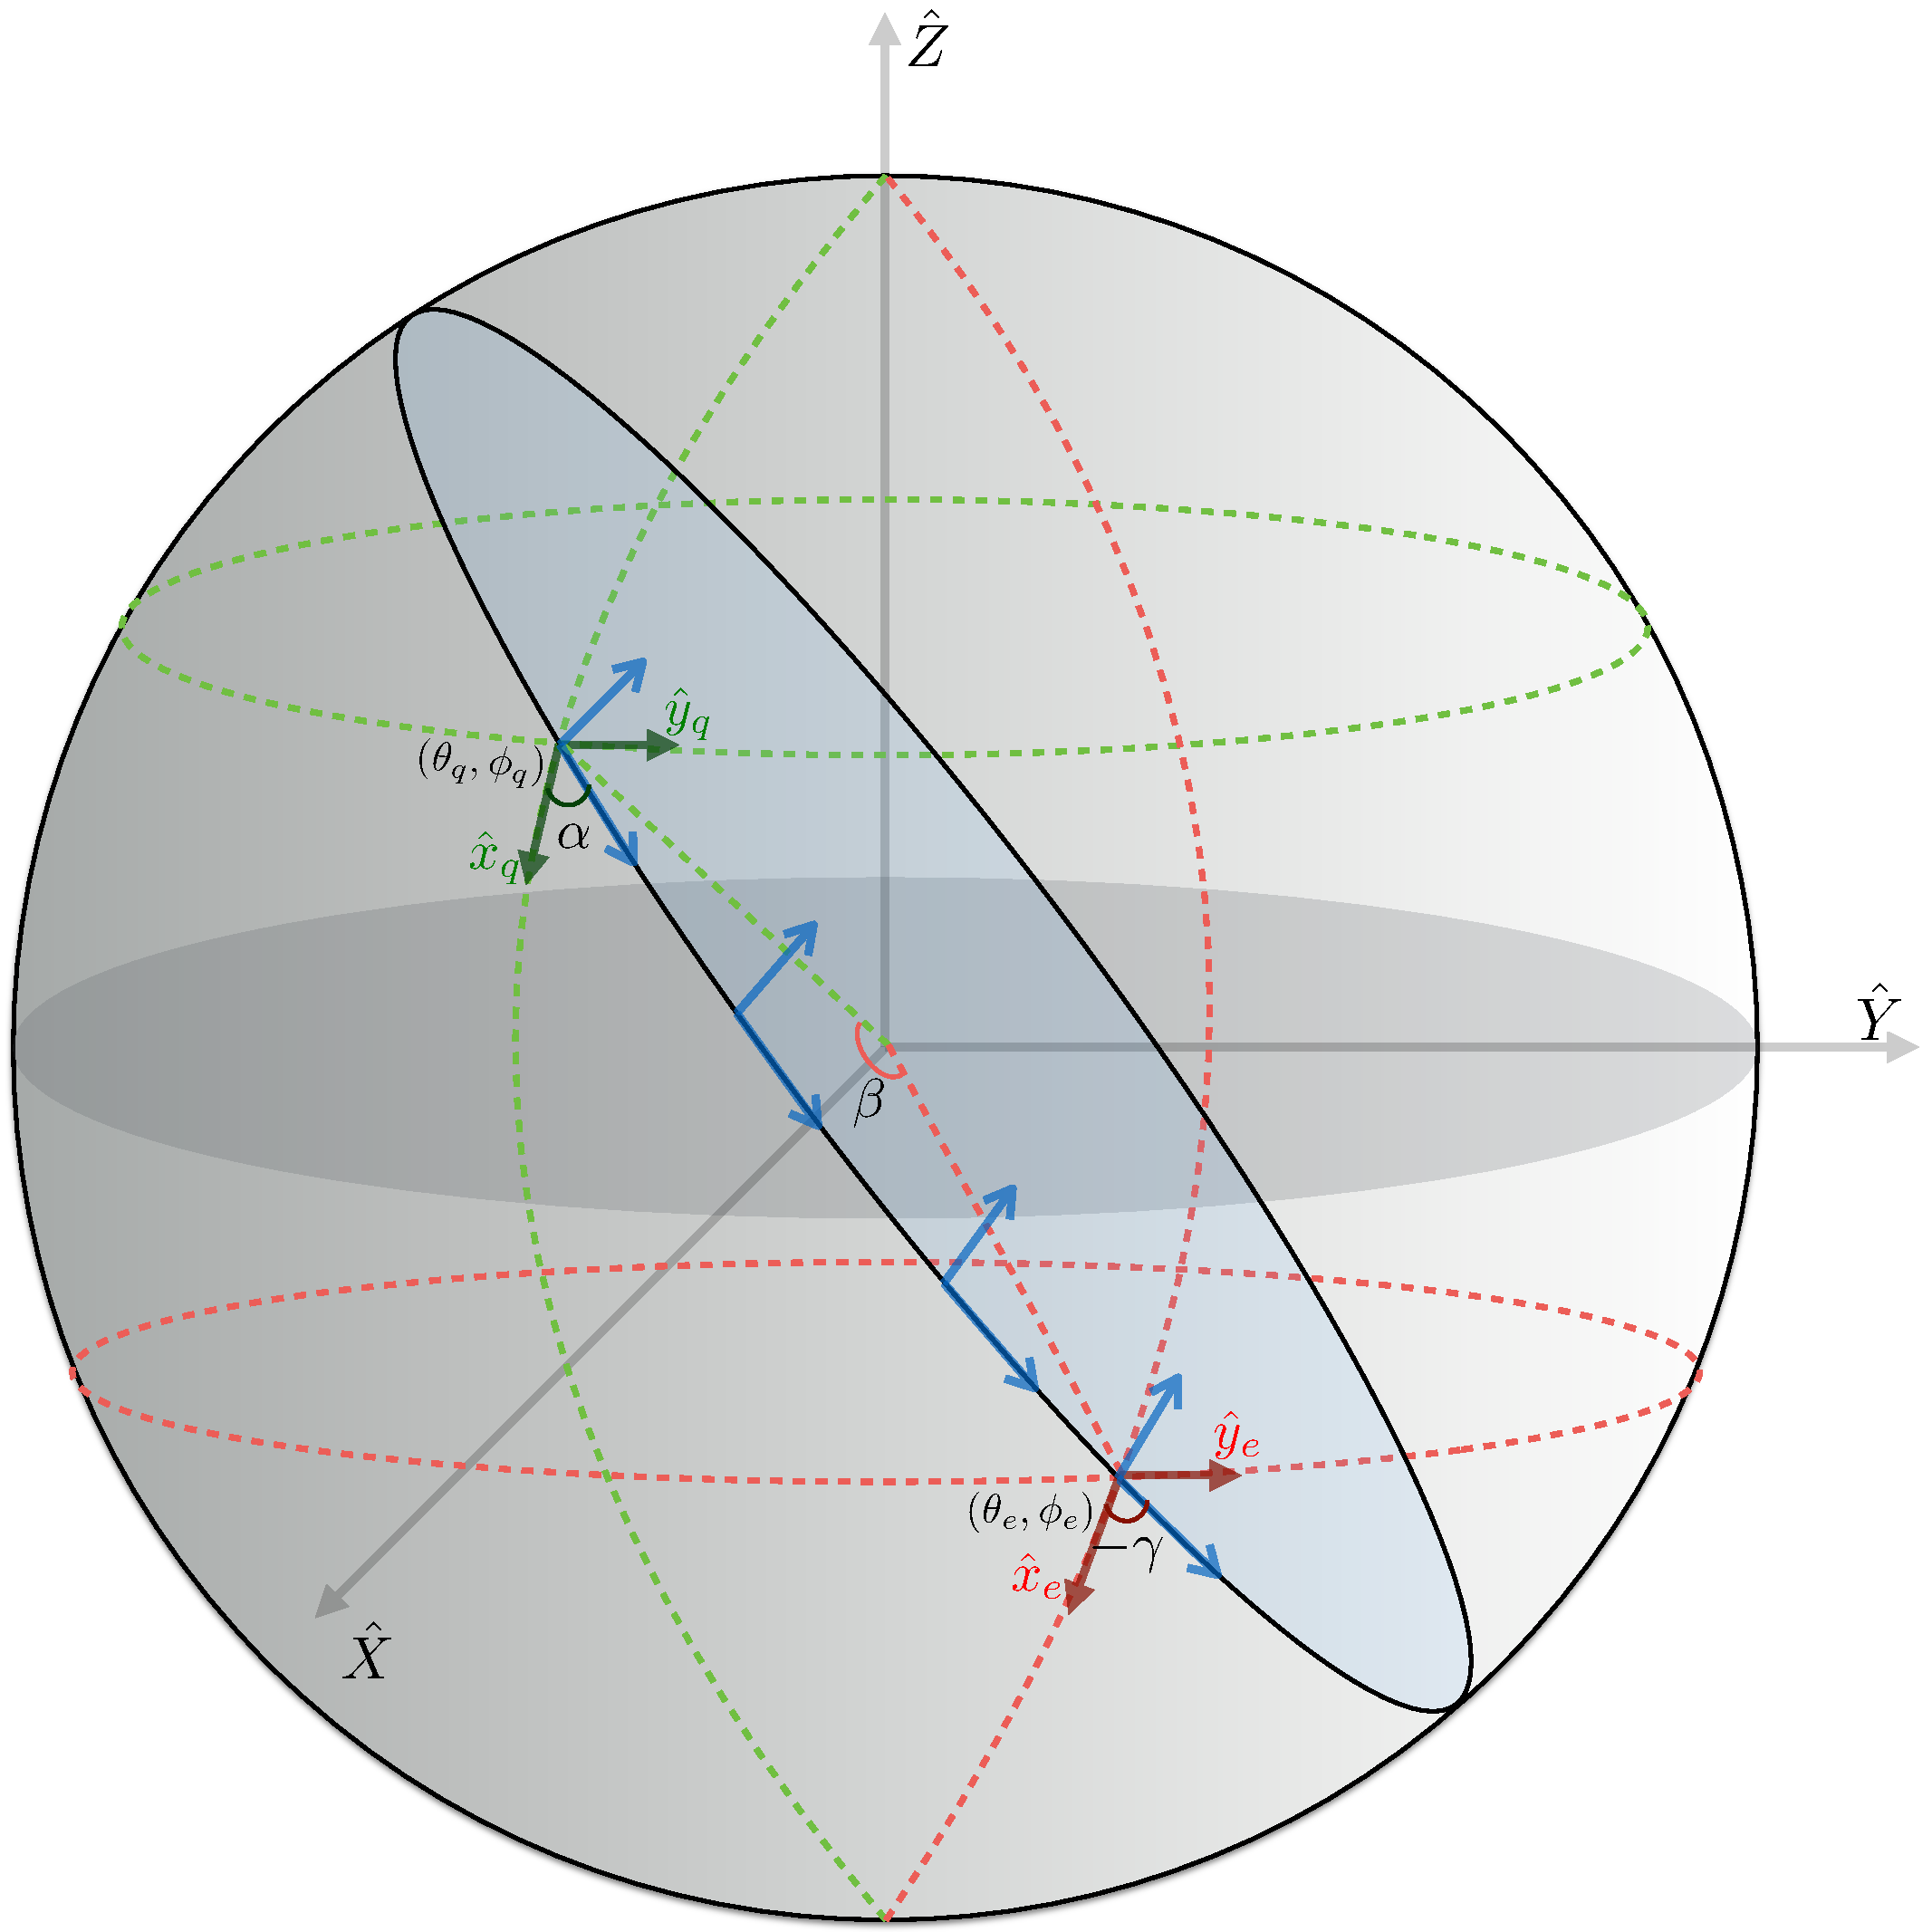
\includegraphics[width=0.5\columnwidth]{euler.pdf}
\caption{This figure depicts the Euler angles in the z-y1-z2 convention. The cartesian coordinates shown in dark green are those that lie in the tangent plane at location $\hat{n}_q = (\theta_q, \phi_q)$ while those shown in dark red are the ones that lie in the tangent plane at location $\hat{n}_e = (\theta_e, \phi_e)$. The blue coordinates at different locations are representative of the parallel transport along the geodesic connection the two locations $\hat{n}_q$ \& $\hat{n}_e$ on the sphere.}
\label{fig:euler_angles}
\end{figure}
%
 
Rotating the cartesian coordinates in the tangent plane at location $\hat{n}_q$ by an angle $\phi$ about the local $\hat{z}_q$ axis, the Stokes parameters in the new coordinate system relate to those in the original coordinate system as:
$\mathcal{R}_{\hat{z}_q}(\phi)[{}_{+2}X(\hat{n}_q)] =  {}_{+2}X(\hat{n}_q) e^{-i2\phi} $.
This same rotation by $\phi$ alters the Euler angle $\alpha_{qe}$ (that aligns the $x$-axis at $\hat{n}_q$ along the geodesic to the location $\hat{n}_e$): $\mathcal{R}_{\hat{z}_q}(\phi)[\alpha_{qe}] = \alpha_{qe} - \phi$.  Therefore one can see that $\mathcal{R}_{\hat{z}_q}(\phi)[e^{-i2\alpha_{qe}}] =  e^{-i2\alpha_{qe}} e^{i2\phi}$.

Given these transformation properties, the combination ${}_{+2}X(\hat{n}_q)e^{-i2\alpha'_{qe}}$ is invariant under rotations and must be spin-0 by definition:
\beq
\mathcal{R}_{\hat{z}_q}(\phi)[{}_{+2}X(\hat{n}_q)e^{-i2\alpha'_{qe}}] = {}_{+2}X(\hat{n}_q) e^{-i2\alpha_{qe}}
\eeq
The real part of the function is constructed by product of functions $(Q\cos{2\alpha}, U\sin{2 \alpha})$ having the same parity and hence the real part must have even parity.  At the same time, the imaginary part of the function is constructed by multiplying functions $(Q\sin{2 \alpha}, U\cos{2\alpha})$ of opposite parity and hence must have an odd parity. Therefore we can make the association that contributions to  $(E+iB)(\hat n_e)$ must be proportional to $ {}_{+2}X(\hat{n}_q) e^{-i2\alpha_{qe}}$.


The same rotation $\mathcal{R}_{\hat{z}_q}(\phi)$ leaves the Euler angle $|\beta_{qe}|$ unaltered (it measures the angular distance between the points).  Thus we can conclude that the contribution to $(E+iB)(\hat n_e)$ from the position $n_q$ must have the form 
\beq
{}_{+2}X(\hat{n}_q) f(\beta_{qe})  e^{-i2\alpha_{qe}}
\eeq
for some real function $f$.  Note that when the two locations coincide ($\beta_{qe}=0$) then  $\alpha_{qe}=0,2\pi,4\pi,\dots$, implying $E + iB \propto Q+iU$.  This is a contradiction because $Q+iU$ does not transform as a spin-0 field under local rotations, and so we must have $f(\beta_{qe} = 0 ) = 0$. A similar contradiction arises when the two locations are diametrically opposite, $\beta_{qe} = \pi$, and so $f(\beta_{qe} = \pi ) = 0$.  Hence the $E/B$ fields are necessarily non-local.  Any such function $f$ will give us $E/B$-like scalar fields.  Below we derive the particular one that gives rise to our familiar $E/B$ modes.

This type of construction can be generalized to transform a field of any spin to a field of any other spin, not just two and zero, and so we can use a similar construction (in the opposite direction) to transform $E/B$ maps back to the Stokes parameters (i.e. transforming spin-0 fields to spin-2).

The kernel's azimuthal part depends only on the Euler angle $\alpha_{qe}$, and so its harmonic transform has no multipole $\ell$ dependence.  The azimuthal part is the crucial operation that translates between different spin representation of CMB polarization. Only the radial part of the kernel $f(\beta_{qe})$ depends only on the angular separation between locations and hence must completely incorporate all the multipole $\ell$ dependence. 

%--------------------------------------------------------
\subsection{Standard $E$/$B$ fields} \label{sec:mat_pol_intro}


The standard construction of $E/B$ fields depend on the spin-raising and -lowering operators, and is usually carried out in harmonic space.  The spin-raising operator ($\eth$), applied to a field of spin-s $_{s}g$, results in a fields with spin-$(s+1)$: $(\eth _{s}g)' = e^{-i(s+1)\psi}(\eth _{s}g)$  \cite{goldberg67}.  The complementary spin-lowering operator $(\bar{\eth})$  similarly results with $(\bar{\eth} _{s}g)' = e^{-i(s-1)\psi}(\bar{\eth} _{s}g)$.  The complex spin-0 scalar now arise from  the spin-2 fields ${_{\pm 2}X}$ as follows,
%
\begin{subequations}\label{eq:ebdef}
\beqry
\mathcal{E}(\hat{n}) + i \mathcal{B}(\hat{n}) &=& -\bar{\eth}^2 _{+ 2}\bar{X}(\hat{n}) \,,\label{eq:ebdef_lower}\\
\mathcal{E}(\hat{n}) - i \mathcal{B}(\hat{n}) &=& -{\eth}^2 _{-2}\bar{X}(\hat{n}) \,.
\eeqry
\end{subequations}
%
%which by the virtue of being scalars are independent of coordinate definitions. %The real part of this complex spin-0 scalar field corresponds to the E-mode while the imaginary part to the B-modes \cite{Kamionkowski1997}. 
The $\cal E/B$ fields are defined locally at point $\hat n$ in terms of the derivative operators $\eth$ and $\bar \eth$.

The complex field $_{\pm 2}X$ defined on the sphere can be decomposed in spin spherical harmonic functions: ${}_{\pm 2}X(\hat{n}) = \sum_{\ell m} {}_{\pm 2} X_{\ell m} {}_{\pm 2}Y_{\ell m}(\hat{n})$. On applying the spin raising and lowering operators on the spin spherical harmonic functions leads to the following identities \cite{goldberg67},
%
\begin{subequations}\label{eq:spinopylm} 
\beqry
\eth _s Y_{lm}(\hat{n}) &=& \sqrt{(\ell-s)(\ell+s+1)} _{s+1} Y_{lm}(\hat{n}) \,, \\
\bar{\eth} _s Y_{lm}(\hat{n}) &=& -\sqrt{(\ell+s)(\ell-s+1)} _{s-1} Y_{lm}(\hat{n}) \,, 
\eeqry
\end{subequations}
%
where $_s Y_{lm}(\hat{n}) $ denote the spin-s spherical harmonics.

Using the definition of $\mathcal{E/B}$, the spin spherical harmonic decomposition of ${}_{\pm2}X$ and the identities given in \eq{eq:spinopylm} it can be shown that the scalar fields $\mathcal{E}/\mathcal{B}$ are given by the following equations,
%
\beq \label{eq:pseudo}
\mathcal{E}(\hat{n}) = \sum_{\ell m} a^{E}_{\ell m} \sqrt{\frac{(\ell+2)!}{(\ell-2)!}} Y_{\ell m} (\hat{n}) ~\,;~ \mathcal{B}(\hat{n})  =\sum_{\ell m} a^{B}_{\ell m} \sqrt{\frac{(\ell+2)!}{(\ell-2)!}} Y_{\ell m} (\hat{n}) \,,
\eeq
%
where the harmonic coefficients $a^{E}_{\ell m}$  \& $a^{B}_{\ell m}$ are related to the harmonic coefficients of the spin-2 polarization field via the following equations,
%
\beq\label{eq:x2eb}
a^{E}_{\ell m} = -\frac{1}{2} \Big[ {}_{+2}\tilde{X}_{\ell m} + {}_{-2}\tilde{X}_{\ell m} \Big] ~\,;~a^{B}_{\ell m} = -\frac{1}{2i} \Big[ {}_{+2}\tilde{X}_{\ell m} - {}_{-2}\tilde{X}_{\ell m} \Big] \,.
\eeq
%
In the remainder of this article, we will work with the scalar $E$ and pseudo scalar $B$ fields as defined by the following equations, 
%
\beq \label{eq:realeb}
E(\hat{n}) = \sum_{\ell m} a^{E}_{\ell m} Y_{\ell m} (\hat{n}) ~\,;~ B(\hat{n})  =\sum_{\ell m} a^{B}_{\ell m} Y_{\ell m} (\hat{n}) \,.
\eeq
%
These $E/B$ fields are merely red-filtered versions of $\mathcal{E}/\mathcal{B}$ (their spherical harmonic coefficients of expansion are related by the factor $[{(\ell+2)!}/{(\ell-2)!}]^{1/2}$), and are not local functions of Stokes $Q,U$. %We make this choice since the CMB spectra are more closely related to the fields E \& B.







\section{Real space polarization operators}
\subsection{Matrix notation} \label{sec:mat_pol_intro}
Our derivation of real space operators is more transparent in a matrix-vector notation.\footnote{While we work with the matrix and vector sizes given in terms of some pixelization parameter $\rm N_{\rm pix}$, all the relations are equally valid in the continuum limit attained by allowing $\rm N_{\rm pix}\rightarrow \infty$}
We introduce a matrix that encodes spin spherical harmonic basis vectors,
%
\beq
{}_{|s|}\mathcal{Y}= \bmat _{+s}Y & 0 \\ 0 & _{-s}Y \emat _{2 \rm N_{\rm pix} \times 2 \rm N_{\rm alms}} \,%,
\eeq
%
%where $s$ denotes the spin of the basis functions.
We will be working with cases $s \in [0,2]$. Each column maps to a specific harmonic basis function (i.e. indexed by $\ell m$) and each row maps to a pixel on the sphere. This matrix is not square in general: the number of rows is determined by the pixelization and the number of columns is set by the number of basis functions (e.g. determined by the band limit).

We now define the different polarization data vectors and their representation in real  space as and harmonic as follows,\footnote{We adopt a convention in which real space quantities are denoted by bar-ed variable while those in harmonic space are denoted by tilde-ed variables.}
%
\beqrys
\bar{S} &=& \bmat E \\ B  \emat_{2 \rm N_{\rm pix} \times 1} ~~~~;~~ \bar{X} = \bmat _{+2}X \\ _{-2}X \emat_{2 \rm N_{\rm pix} \times 1} ~~;~~\bar{P} =\fqu_{\tiny {2 \rm N_{\rm pix} \times 1}} \,, \\
\tilde{S} &=& \bmat a^{E} \\ a^{B} \emat _{2 \rm N_{\rm alms} \times 1}  ~~; ~~ \tilde{X} = \bmat _{+2} \tilde{X} \\ _{-2} \tilde{X} \emat_{2 \rm N_{\rm alms} \times 1} \,.
\eeqrys
%
The different symbols have the same meaning as that discussed in \sec{sec:pol-primer}, except that the subscript ${\ell m}$ for the spherical harmonic coefficients is suppressed for cleaner notation.

We define transformations between different representations of the polarization field (i.e. from $Q,U$ to $_{\pm2} X$):
%
\beqrys
\bar T &=& \qutox_{2 \rm N_{\rm pix} \times 2 \rm N_{\rm pix}} ~~;~~ \bar T^{-1} = \frac{1}{2} \bar T^{\dagger} \,, \\
\tilde T &=& -\qutox_{2 \rm N_{\rm alms} \times 2 \rm N_{\rm alms}} ~~;~~ \tilde T^{-1} = \frac{1}{2} \tilde T^{\dagger} \,,
\eeqrys
%
The sign conventions we have chosen match HEALPix.
Using the data vectors and the matrix operators defined above we can now express, in compact notation, the forward and inverse relations between different representations of the polarization data vectors as follows,
%
\begin{subequations} \label{eq:pol_data_relns}
  %Kevin's version
  \beqry
  \bar{X} &= \bar T  \bar{P}; &\qquad \bar{P} = \frac{1}{2} \bar T^{\dagger}  \bar{X} ; \\
  \tilde{X} &= \tilde T \tilde{S}; &\qquad \tilde{S} = \frac{1}{2}\tilde T^{\dagger} \tilde{X} \,.
  \eeqry
  Meanwhile the spherical harmonic transforms are written as:
  \beqry
  \bar X &=  {{}_2\mathcal{Y}}  \tilde X; &\qquad \tilde X ={{}_2\mathcal{Y}}^{\dagger}  \bar X  ; \\
  \bar S &=  {{}_0\mathcal{Y}} \tilde S; &\qquad  \tilde S =  {{}_0\mathcal{Y}}^{\dagger} \bar S \,.
  \eeqry
% Aditya's version
%\beqry
%\bar{X} &=& \bar T * \bar{P} ~~;~~\bar{P} = \frac{1}{2} \bar T^{\dagger} * \bar{X} \,, \\
%\bar X &=&  {{}_2\mathcal{Y}} * \tilde X  ~~;~~ \tilde X ={{}_2\mathcal{Y}}^{\dagger} * \bar X  \,, \\
%\tilde{X} &=& \tilde T * \tilde{S} ~~;~~ \tilde{S} = \frac{1}{2}\tilde T^{\dagger} * \tilde{X} \,.\\ 
%\bar S &=&  {{}_0\mathcal{Y}} * \tilde S ~~;~~  \tilde S =  {{}_0\mathcal{Y}}^{\dagger} * \bar S \,.
%\tilde X &=&  {{}_2\mathcal{Y}}^{\dagger} * \bar X ~~;~~ \tilde{X} = \tilde T * \tilde{S} \,, \\
%\bar{S} &=& {{}_0\mathcal{Y}}*\tilde S ~~;~~ \tilde{S} = \frac{1}{2}\tilde T^{\dagger} * \tilde{X} \,.\\
%\bar{X} &=& \bar T * \bar{P} ~~;~~ \tilde{X} = \tilde T * \tilde{S} \,, \\
%\bar{P} &=& \frac{1}{2} \bar T^{\dagger} * \bar{X} ~~;~~ \tilde{S} = \frac{1}{2}\tilde T^{\dagger} * \tilde{X} \,. \\
%\eeqry
\end{subequations}
%
Finally we introduce the operators that project harmonic space data vector to the $E$ or $B$ subspace,
%
\begin{subequations} \label{eq:har_eb_op}
\beqry
\tilde O_E &=& \bmat \mathbb{1} & \mathbb{0} \\ \mathbb{0} & \mathbb{0} \emat _{2 \rm N_{\rm alms} \times 2 \rm N_{\rm alms} }   ~~;~~ \tilde S_E = \tilde O_E  \tilde S ,\\
\tilde O_B &=& \bmat \mathbb{0} & \mathbb{0} \\ \mathbb{0} & \mathbb{1} \emat _{2 \rm N_{\rm alms} \times 2 \rm N_{\rm alms} } ~~; ~~ \tilde S_B = \tilde O_B  \tilde S .
\eeqry
\end{subequations}
%
Note that these harmonic space matrices are idempotent ($\tilde O_E  \tilde O_E = \tilde O_E;  \tilde O_B  \tilde O_B= \tilde O_B$), orthogonal ($\tilde O_E  \tilde O_B = \mathbb{0}$), and sum to the identity matrix ($\tilde O_E + \tilde O_B = \mathbb{1}$).
%
%\begin{subequations} \label{eq:har_op_prop}
%\beqry
%\tilde O_E  \tilde O_E&=& \tilde O_E ~~;~~  \tilde O_B  \tilde O_B= \tilde O_B \,,\\
% \tilde O_E  \tilde O_B&=& \mathbb{0} \,, \label{eq:op_eb_ortho}\\ 
% \tilde O_E + \tilde O_B&=& \mathbb{1} \,.
%\eeqry
%\end{subequations}
%
The above relations for these harmonic space operators are exactly valid.  In the following sections we aim to derive the real space analogues ($O_E,O_B$) of these harmonic space operators.



\subsection{Evaluating scalar fields $E$ \& $B$ from Stokes parameters $Q$ \& $U$}\label{sec:qu2eb}
In \sec{sec:pol-primer} we described the conventional procedure of computing the scalar fields E \& B from the Stokes parameters Q \& U. 
%To reiterate, this process involved taking the spin harmonic transform of the complex spin-2 fields ${}_{\pm2} \bar X$, forming specific linear combinations of the resultant coefficients of expansion ${}_{\pm 2} \tilde X_{\ell m}$ and evaluating the forward spin-0 transform to derive the scalar E \& B fields. 
In this section we derive the real space convolution kernels on the sphere which can be used to directly evaluate the scalar fields $E$ \& $B$ on the sphere.  We use the vector-matrix notation introduced in \sec{sec:mat_pol_intro} to write down an operator equation relating the real space vector of scalars \vs to the Stokes polarization vector \vp{},
%
\beqrys
\bar{S} &=& {{}_0\mathcal{Y}} *\tilde T^{-1}* {{}_2\mathcal{Y}^{\dagger}} *\bar T *\bar{P} = \frac{1}{2} {{}_0\mathcal{Y}} *\tilde T^{\dagger} *{{}_2\mathcal{Y}^{\dagger}} *\bar T *\bar{P}   \,, \\
&=&  \bar O *\bar{P} \,. \label{eq:qu2eb_op}
\eeqrys
%
The explicit form of the real space operator $\bar O$ can be derived by contracting over all the matrix operators. This procedure is explicitly worked out in the following set of equations,
%
\beqrys
\bar{O} &=& \frac{1}{2} {{}_0\mathcal{Y}} *\tilde T^{\dagger} *{{}_2\mathcal{Y}^{\dagger}} *\bar T \,, \\
&=& -0.5 \yzmat{e} \qutoxd \ymatc{q} \qutox   \,, \\
&=& -0.5 \begin{bmatrix} \sum ({}_{0}Y_e ~{}_{2}Y^{T*}_q  +  {}_{0}Y_e~ {}_{-2}Y^{T*}_q) & {\rm i}  \sum ({}_{0}Y_e ~ {}_{2}Y^{T*}_q - {}_{0}Y_e ~{}_{-2}Y^{T*}_q)  \\  - {\rm i} \sum  ({}_{0}Y_e ~ {}_{2}Y^{T*}_q - {}_{0}Y_e~ {}_{-2}Y^{T*}_q) & \sum ({}_{0}Y_e~ {}_{2}Y^{T*}_q + {}_{0}Y_e ~{}_{-2}Y^{T*}_q)  \end{bmatrix} \,, \label{eq:qu2eb_ker_1}
\eeqrys
%
where the symbol ${}_{0}Y_e$ is used to denote the sub-matrix ${}_{0}Y_{\hat{n}_e \times \ell m} \equiv {}_{0}Y_{\ell m}(\hat{n}_e)$, the symbol ${}_{\pm 2}Y^{T*}_q$ is used to denote the transposed conjugated matrix ${}_{\pm 2}Y^*_{\ell m \times \hat{n}_q} \equiv {}_{\pm 2}Y^*_{\ell m}(\hat{n}_q)$ and the summation is over the multipole indices $\ell,m$. Note that here we purposefully introduce the notation of the index ``e'' to denote the location where the scalar fields are being evaluated and the index ``q'' to denote the location from which  the Stokes parameters are being accessed. Using the conjugation properties of the spin spherical harmonic functions it can be shown that the following identity holds true,
%
\beq
 \left [\sum_{\ell m} {}_{0}Y_{\ell m}(\hat{n}_e){}_{+2}Y^*_{\ell m}(\hat{n}_q)\right]^* = \sum_{\ell m} {}_{0}Y_{\ell m}(\hat{n}_e){}_{-2}Y^*_{\ell m}(\hat{n}_q) \,,
 \eeq
 %
where the terms on either side of the equation are those that appear in \eq{eq:qu2eb_ker_1}. Note that the operator $\bar{O}$ is real as one expects, since each sub-matrix in \eq{eq:qu2eb_ker_1} is formed by summing a complex number and its conjugate. 

\noindent \eq{eq:qu2eb_ker_1} already presents a real space operator, but it is not in a form which can be practically implemented. To arrive at a real space operator which is practially usable, we use the fact that the $m$ sum over the product of two spin spherical harmonic functions can be expressed as a function of the Euler angles\cite{varshalovich},
%
\beq \label{eq:sum_spin_shf}
 \sum_{m}{{}_{s_1}Y}^*_{\ell m}(\hat{n}_i)\,{{}_{s_2}Y}_{\ell m}(\hat{n}_j) = \sqrt{\frac{2\ell+1}{4 \pi}} {{}_{s_2}}Y_{\ell \,-s_1}(\beta_{ij},\alpha_{ij}) e^{- i s_2 \gamma_{ij}} \,,
\eeq
%
where $\alpha_{ij}, ~\beta_{ij} ~\&~ \gamma_{ij}$ denote the Euler angles that specifically transform $(i \rightarrow j)$: the coordinate system at $\hat{n}_i$ so as to allign the coordinate system at $\hat{n}_j$\footnote{The sense of the rotation become more obvious when this equation is written in terms of the Wigner-D functions.}. The different parts of the real space operator $\bar{O}$  are completely specified by the complex function,
%
\begin{subequations}\label{eq:qu2eb_gen_kernel}
\beqry
\mathcal{M}( \hat{n}_e, \hat{n}_q)  &=& \mathcal{M}_{r} + i \mathcal{M}_{i}  \,,\nonumber \\ 
&=&\sum_{\ell m} {{_0}Y}_{\ell m}(\hat n_e) \, {{_{-2}}Y}^*_{\ell m}(\hat n_q) = \sum_{\ell} \sqrt{\frac{2\ell+1}{ 4 \pi}}{{_0Y}_{\ell 2}}(\beta_{qe},\alpha_{qe})\,,\\
&=&  \Big [ \cos(2 \alpha_{qe}) + i \sin(2 \alpha_{qe} ) \Big]   \sum_{\ell=\ell_{\rm min}}^{\ell_{\rm max}} {\frac{2\ell+1}{ 4 \pi}} \sqrt{\frac{(\ell-2)!}{(\ell+2)!}}P_{\ell 2} (\cos\beta_{qe}) \,, \label{eq:rad_ker_queb} \\
&=&  \Big [ \cos(2 \alpha_{qe}) + i \sin(2 \alpha_{qe} ) \Big] {{}_{\mm}f}(\beta_{qe},\ell_{\rm min},\ell_{\rm max}) \,, 
\eeqry
\end{subequations}
%
where we have used the identity in \eq{eq:sum_spin_shf} to simplify the product of the spherical harmonic functions. Note that the function on the right depends only on two out of the three Euler angles. Employing \eq{eq:qu2eb_gen_kernel} to simplify the product of spherical harmonic functions in \eq{eq:qu2eb_ker_1}, the real space operator $\bar{O}$ can now be cast in this more useful form,
%
\beq\label{eq:op_qu2eb_rad}
\bar O =-\bmat  \mathcal{M}_{r} & \mathcal{M}_{i} \\  -\mathcal{M}_{i}  & \mathcal{M}_{r} \emat_{2 N_{\rm pix} \times 2 N_{pix}} = -{{}_{\mm}f}(\beta_{qe},\ell_{\rm min},\ell_{\rm max})\bmat \cos(2 \alpha_{qe}) & \sin(2\alpha_{qe})\\  -\sin(2 \alpha_{qe})  & \cos(2 \alpha_{qe}) \emat \,,
\eeq
%
where, we reiterate, $\alpha_{qe}, ~\beta_{qe} ~\&~ \gamma_{qe}$ denote the Euler angles which rotate the local cartesian system at $\hat{n}_q$ (location where Stokes parameters are accessed) to the cartesian system at  $\hat{n}_e$ (location where the scalar fields are evaluated): $\hat{n}_q \xrightarrow{\mathcal{R}(\alpha_{qe},\beta_{qe},\gamma_{qe})} \hat{n}_e$. 

\textit{Radiating kernel:} Using \eq{eq:op_qu2eb_rad} in \eq{eq:qu2eb_op} one can see that the $E$/$B$ contribution of the Stokes parameters at some location $\hat{n}_q$ is given by the following expression,
%
\beq  \label{eq:qu2eb_radiation_explicit}
\bar{S}_q = \bmat E_e \\ B_e  \emat_{q} =- {{}_{\mm}f}(\beta_{qe},\ell_{\rm min},\ell_{\rm max})\bmat \cos(2 \alpha_{q e}) & \sin(2\alpha_{q e})\\  -\sin(2 \alpha_{q e})  & \cos(2 \alpha_{q e}) \emat  \bmat Q_{q} \\ U_{q}  \emat \Delta \Omega \,.
\eeq
%
The total map of E \& B modes can be simply evaluated by summing over the contribution from the Stokes parameters at each location $\hat{n}_q$ : $\bar{S} = \sum_{q=1}^{N_{\rm pix}} \bar{S}_q$. This operation can be cast in a concise form as follows,
%
\begin{subequations} \label{eq:qu2eb_radiation_concise}
\beqry 
\left[E + iB\right](\hat{n}_e) &=& -\Delta \Omega  \sum_{q=1}^{N_{\rm pix}} \Big[ {}_{+2}X(\hat{n}_{q}) e^{-i2\alpha_{q e}} \Big]  {{}_{\mm}f}(\beta_{q e}) \,, \\
&=&    \sum_{q=1}^{N_{\rm pix}} \Bigg\lbrace {}_{+2}X(\hat{n}_{q}) \cdot \left[ - \Delta \Omega \sum_{\ell=\ell_{\rm min}}^{\ell_{\rm max}} \sqrt{\frac{2 \ell+1}{4 \pi}}Y^*_{\ell 2}(\beta_{qe},\alpha_{qe}) \right] \Bigg\rbrace \,, \\
&=& \sum_{q=1}^{N_{\rm pix}} {}_{+2}X(\hat{n}_{q}) \cdot  \mathcal{M}_{G}[\hat{n}_q] \,,
\eeqry
\end{subequations}
%
where ``$\cdot$'' denotes a simple scalar multiplication. $\mathcal{M}_{G}$ is merely the conjugated function $\mm^*$ when expressed as a function of the Euler angle $\alpha_{qe}$ and it can be thought of as the Green's function of the operator, since $[E +iB] = \mathcal{M}_{G}$ is the spin-0 scalar field generated from the Stokes charge $[Q+iU] = [\delta(\hat{n}-\hat{n}_q) + i 0]$. 

We denote the kernel expressed in terms of the Euler angle $\alpha$ as the radiating kernel, since it allows us to evaluate the $E/B$ field contribution across the sphere due to a single Stoke (charge) parameter at a fixed location on the sphere. The total $E/B$ maps can then be thought of as just superposed radiation emerging from Stokes charges across the sphere. In this formulation, one is effectively in the frame of the Stokes charge ${}_{\pm2}X$ and evaluating its contribution to the complex spin-0 scalar field across the sphere. 
%
\begin{figure}[!t]
\centering
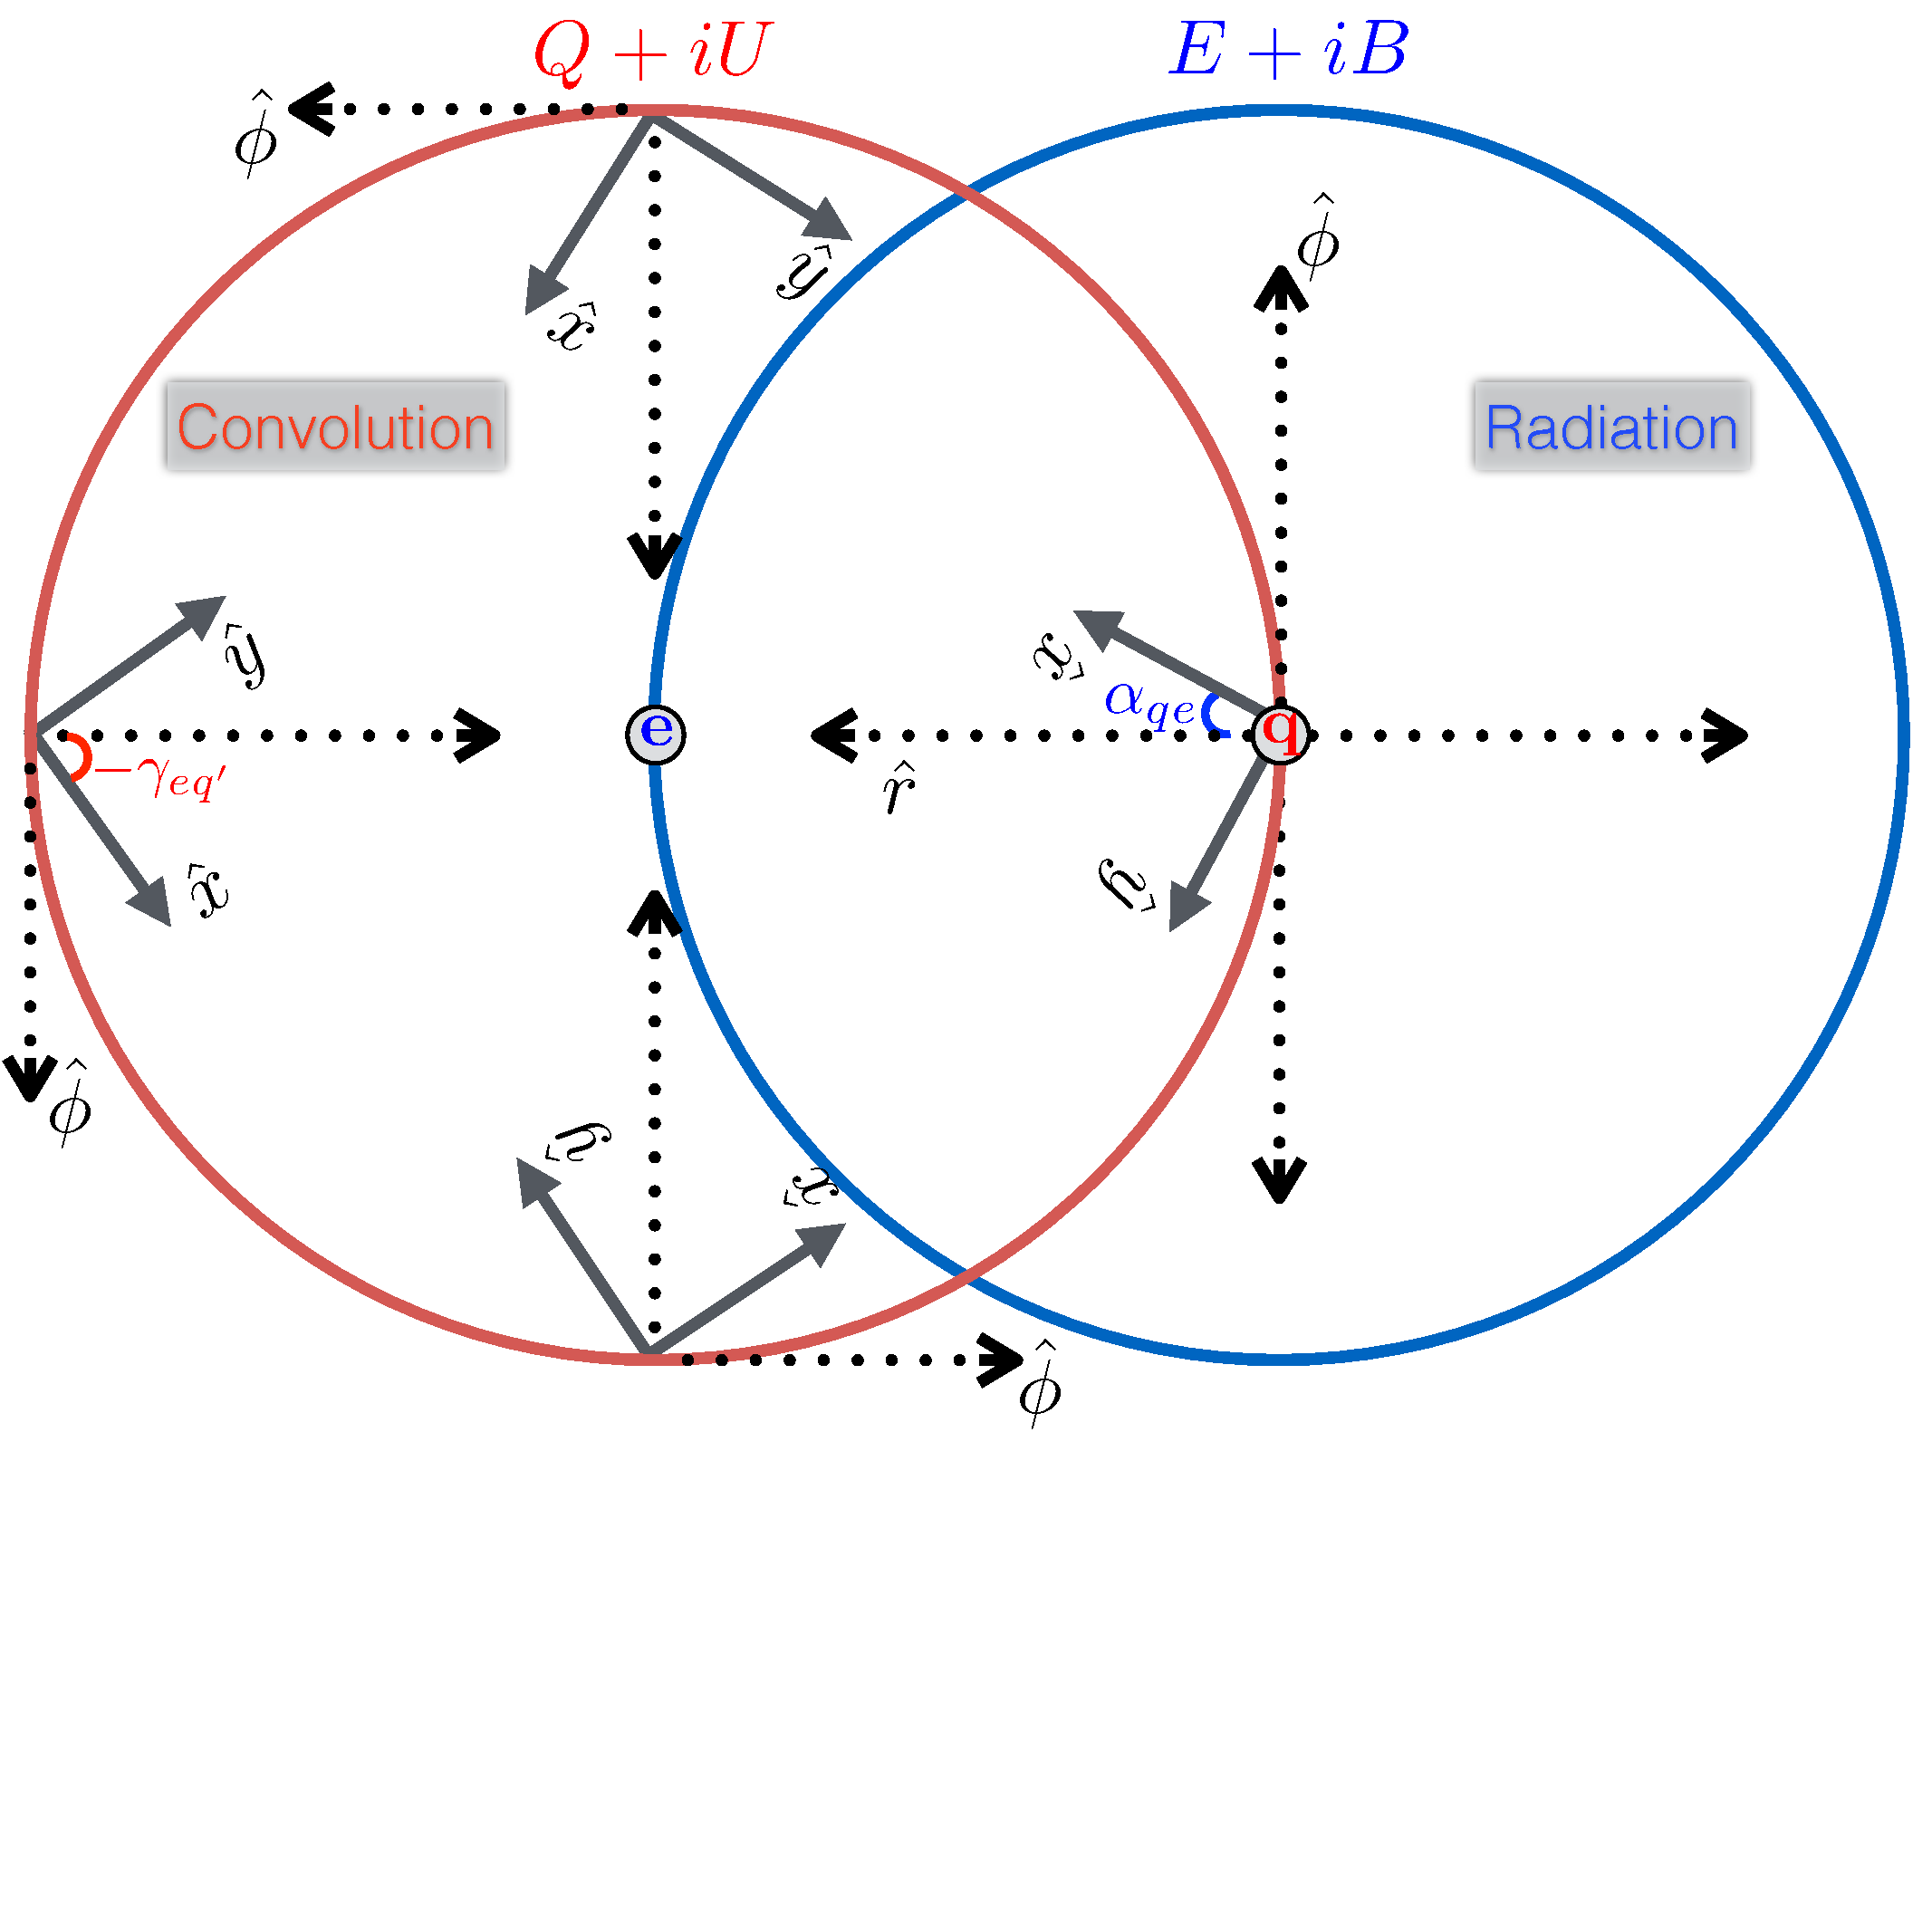
\includegraphics[width=0.5\columnwidth]{radiation_convolution.pdf}
\caption{The local cartesian coordinate are only drawn on the red circle, representative of the coordinate dependence of the Stokes parameters. The value of the scalar field at location `e' can be evaluated by summing over the contribution from all the Stokes parameters on the red circle (sphere). The convolutions are performed with kernels which are defined in term of the Euler angle $\gamma_{eq}$. Alternatively, one can compute the contribution from the Stokes parameter at location `q' to all the point on the blue circle(sphere) and this is a function of the Euler angle $\alpha_{eq}$. In the flat sky limit, since $\gamma=-\alpha$ there is no difference between the radiating and convolving kernels.}
\label{fig:planar_euler_angles}
\end{figure}
%

\textit{Convolution kernel:} We can also formulate the real space operator to be a function of Euler angles corresponding to the inverse rotation. The Euler angles for the inverse rotations (i.e. to align the coordinate system at $\hat{n}_e$ with that at $\hat{n}_q$) are related to the forward rotation Euler angles by the following relations: $\alpha_{eq}=-\gamma_{qe}$, $\beta_{eq} = -\beta_{qe}$ and  $\gamma_{eq} =-\alpha_{qe}$. Since the kernel only depends on the cosine of the Euler angle $\beta$, it is immune to changes in its sign. The operator equation can be expressed as a function of the Euler angle $\gamma_{eq}$ as follows, 
%
\beq \label{eq:qu2eb_convolution_explicit}
\bmat E_e \\ B_e  \emat =- \sum_{q=1}^{N_{\rm pix}}{{}_{\mm}f}(\beta_{eq},\ell_{\rm min},\ell_{\rm max})\bmat \cos(2 \gamma_{eq}) & -\sin(2\gamma_{eq})\\  \sin(2 \gamma_{eq})  & \cos(2 \gamma_{eq}) \emat  \bmat Q_q \\ U_q  \emat \Delta \Omega\,,
\eeq
%
%where $\Delta \Omega$ denotes the pixel area and all the symbols have their usual meaning. 
\revisit{This version of the real space operator would have naturally emerged had we simplified the the equivalent function $\sum_{\ell m} {}_{0}Y^*_{\ell m}(\hat{n}_e){}_{+2}Y_{\ell m}(\hat{n}_q)$ in \eq{eq:qu2eb_gen_kernel}.} This formulation of the real space operator can be interpreted as integrating at some fixed location $\hat{n}_e$ the $E/B$ mode contribution arising from the Stokes parameters at all location $\hat{n}_q$ on the sphere. This operation can be expressed more concisely as follows,
%
\begin{subequations} \label{q:qu2eb_convolution_concise}
\beqry 
[E + iB](\hat{n}_e) &=& - \Delta \Omega \sum_{q=1}^{N_{\rm pix}} \left(\sum_{\ell=\ell_{\rm min}}^{\ell_{\rm max}} \frac{2 \ell+1}{4 \pi} \sqrt{\frac{(\ell-2)!}{(\ell+2)!}} P_{\ell}^{2}(\beta_{eq}) \right) {\Bigg( e^{i2 \gamma_{eq}}   {}_{+2}X (\hat{n}_q) \Bigg)} \,, \label{eq:qu2eb_physical}\\
&=& \Bigg\lbrace \left[ - \Delta \Omega \sum_{\ell=\ell_{\rm min}}^{\ell_{\rm max}} \sqrt{\frac{2 \ell+1}{4 \pi}}Y_{\ell 2}(\beta_{eq},\gamma_{eq}) \right]  \circ {}_{+2}X \Bigg\rbrace(\hat{n}_e) \,, \\
&=& \Bigg\lbrace \mathcal{M}_{B} \circ {}_{+2}X \Bigg\rbrace(\hat{n}_e) \,, \label{eq:qu2eb_convolution} 
\eeqry
\end{subequations}
%
where $\circ$ denotes a convolution and $\mathcal{M}_{B}$ is merely the conjugated function $\mm^*$ when expressed as a function of the Euler angle $\gamma_{eq}$ it can be thought of as an effective instrument beam pointing to the direction $\hat{n}_e$. 
%--------------------------------------------------------


%--------------------------------------------------------
\subsection{Evaluating Stokes parameters $Q$ \& $U$ from scalar fields $E$ \& $B$}\label{sec:eb2qu}
The real space operator which translates $E$ \& $B$ fields to Stokes parameters $Q$ \& $U$ can be derived using a similar procedure. Expressed in the matrix-vector notation, inverse operator is given by,
%
\begin{subequations}
\beqry
\bar{P} &=& \bar{T}^{-1} *{{}_2\mathcal{Y}} *\tilde T *{{}_0\mathcal{Y}^{\dagger}}\bar{S} = \frac{1}{2} \bar{T}^{\dagger} *{{}_2\mathcal{Y}} *\tilde T *{{}_0\mathcal{Y}^{\dagger}}\bar{S} \,,  \\
&=&  \bar O^{-1} *\bar{S}\,.
\eeqry
\end{subequations}
%
%The inverse operator $\bar{O}^{-1}$ can be derived by realizing that $\mm^{-1}$ is given by the following expression,
%%
%\beq
%\mm^{-1} = \sum_{\ell m}  {{}_{2}}Y_{\ell m}(\hat n_q) {}_{0}Y^*_{\ell m}(\hat n_e) \, 
%\eeq
%%
The inverse operator expressed in terms of the function $\mm$ given in \eq{eq:qu2eb_gen_kernel} is given by the following equation,
%
\beq
{\bar O}^{-1}=-\bmat \mathcal{M}_{r} & -\mathcal{M}_{i} \\  \mathcal{M}_{i}  & \mathcal{M}_{r} \emat_{2 N_{\rm pix} \times 2 N_{pix}} =-{{}_{\mm}f}(\beta_{eq},\ell_{\rm min},\ell_{\rm max})\bmat \cos(2 \alpha_{qe}) & -\sin(2\alpha_{qe})\\  \sin(2 \alpha_{qe})  & \cos(2 \alpha_{qe}) \emat \,,
\eeq
%
where all the symbols have the same meaning as discussed in \sec{sec:qu2eb}. Note that the kernel in the above equation differs from the one in \eq{eq:op_qu2eb_rad} by a change in sign on the off-diagonals of the block matrix. When expressed in terms of the same set of Euler angles used to define the operator $\bar{O}$, it can be shown that the different forms of the real space operator are given by,
%
\beqry
{}_{+2}X(\hat{n}_q) &=& \Bigg\lbrace \mathcal{M}^*_{G} \circ [E+iB] \Bigg\rbrace(\hat{n}_q) \hspace{0.8cm} \textrm{\emph {Convolution kernel}}\,, \label{eq:eb2qu_convolution}\\
{}_{+2}X(\hat{n}_q) &=&  \sum_{e=1}^{N_{\rm pix}} [E+iB](\hat{n}_{e}) \cdot  \mathcal{M}^*_{B}[\hat{n}_e] \hspace{0.8cm} \textrm{\emph{Radiation kernel}}\,,
\eeqry
%
where all the symbols have the same meaning as defined in \sec{sec:qu2eb}. Note that the conjugated forms of the Green's function and the effective beam for the operator $\bar{O}$ have their roles reversed for the inverse operator $\bar{O}^{-1}$.
%--------------------------------------------------------


%--------------------------------------------------------
\subsection{Decomposing Stokes parameters $Q$ \& $U$  into those corresponding to $E$ \& $B$ modes respectively}
We can only measure the total Stokes vector which is a sum of the Stokes vectors corresponding to the respective scalar modes. The $E$ \& $B$ modes are orthogonal to each other, in the sense that their respective operators are orthogonal to each other as seen in \eq{eq:op_eb_ortho}. It is possible to decompose the Stokes vector \vp{} into one \vp{\rm E} that purely contributes to $E$ modes and another \vp{\rm B} that purely contribute to the $B$ modes of polarization. In this section we derive the real space operators which operate on the total Stokes vector and yield this decomposition, without ever having to explicitly evaluate the scalar modes. Though the algebra is a little more involved, the derivation is similar to that discussed in \sec{sec:qu2eb}, hence we refrain from presenting the detailed calculations here, but outline the key points. We use the harmonic space projection operators $\tilde O_{E/B}$, defined in \eq{eq:har_eb_op}, to derive the respective real space operators. The Stokes parameters corresponding to each scalar mode are given by the following expressions,
%
\beqry
\bar{P}_E &=&  [\bar T^{-1} * {{}_2\mathcal{Y}} *\tilde T * \tilde O_E* \tilde T^{-1}* {{}_2\mathcal{Y}^{\dagger}} *\bar T] *\bar{P}  \,, \\
&=& [\frac{1}{4} \bar T^{\dagger } * {{}_2\mathcal{Y}} *\tilde T * \tilde O_E* \tilde T^{\dagger} * {{}_2\mathcal{Y}^{\dagger}} *\bar T ]*\bar{P}  \,, \nonumber \\
&=&  \bar O_{E}*\bar{P} \,,\nonumber \\
\bar{P}_B &=&  [\bar T^{-1}* {{}_2\mathcal{Y}}* \tilde T* \tilde O_B* \tilde T^{-1}* {{}_2\mathcal{Y}^{\dagger}}* \bar T]*\bar{P}  \,, \\
&=& [\frac{1}{4} \bar T^{\dagger } * {{}_2\mathcal{Y}} *\tilde T * \tilde O_B* \tilde T^{\dagger} *{{}_2\mathcal{Y}^{\dagger}} *\bar T] *\bar{P}   \,, \nonumber\\
&=&  \bar O_{B}*\bar{P} \,. \nonumber
\eeqry
%
We contract over all the matrix operators to arrive at the the real space operators. On working through the algebra it can be shown that the real space operators have the following form,
%
\beq
\bar O_{E/B} = 0.5 \bmat \mathcal{I}_{r} & \mathcal{I}_{i} \\  -\mathcal{I}_{i}  & \mathcal{I}_{r} \emat \pm 0.5 \bmat \mathcal{D}_{r} & \mathcal{D}_{i} \\  \mathcal{D}_{i}  & - \mathcal{D}_{r} \emat \,,\\
\eeq
where $\mathcal{I}_{r} ~\&~ \mathcal{D}_{r}$ and $\mathcal{I}_{i} ~\&~ \mathcal{D}_{i}$ are the real and complex parts of the following complex functions,
%
\begin{subequations}
\beqry
\mathcal{I} (\hat{n}_e,\hat{n}_q) &=& \mathcal{I}_{r} + i \mathcal{I}_{i} = \sum_{\ell m} {_{-2}Y}_{\ell m}(\hat n_e) {_{-2}Y}^*_{\ell m}(\hat n_q) \,, \\
\mathcal{D}(\hat{n}_e,\hat{n}_q)  &=& \mathcal{D}_{r} + i\mathcal{D}_{i} = \sum_{\ell m} {_2Y}_{\ell m}(\hat n_e) {_{-2}Y}^*_{\ell m}(\hat n_q) \,.
\eeqry
\end{subequations}
%
These functions can be further simplified using the identity of spin spherical harmonics given in \eq{eq:sum_spin_shf}. Specifically it can be shown that these functions reduce to the following mathematical forms,
%
\beqrys \label{eq:fn_i}
\mathcal{I}(\hat{n}_e, \hat{n}_q) &=& \sum_{\ell} \sqrt{\frac{2\ell+1}{ 4 \pi}}{_{-2}Y}_{\ell2}(\beta_{qe}, \alpha_{qe}) ~ \rm{e}^{i2 \gamma_{qe}} \label{eq:healpix-compatible-i} = \mathcal{I}_r + i \mathcal{I}_i \,, \\
\mathcal{I}_r + i \mathcal{I}_i &=& \Big [ \cos(2 \alpha_{qe} +  2\gamma_{qe}) + i \sin(2 \alpha_{qe} +  2 \gamma_{qe}) \Big]   {{}_{\mi}f}(\beta_{qe},\ell_{\rm min},\ell_{\rm max}) \,,
\eeqrys
%
%
\beqrys \label{eq:fn_d}
\mathcal{D}(\hat{n}_q, \hat{n}_e) &=& \sum_{\ell} \sqrt{\frac{2\ell+1}{ 4 \pi}}{_2Y}_{\ell 2}(\beta_{qe}, \alpha_{qe}) ~ \rm{e}^{- i2 \gamma_{qe}} \label{eq:healpix-compatible-m} =\mathcal{D}_r + i \mathcal{D}_i \,, \\
\mathcal{D}_r + i \mathcal{D}_i &=&  \Big [ \cos(2 \alpha_{qe} - 2\gamma_{qe}) + i \sin(2 \alpha_{qe} -  2 \gamma_{qe}) \Big]   {{}_{\md}f}(\beta_{qe},\ell_{\rm min},\ell_{\rm max}) \,,
\eeqrys
%
where the radial functions are given by,
%
\beq
{{}_{\mdi}f}(\beta,\ell_{\rm min},\ell_{\rm max}) = \sum_{\ell=\ell_{\rm min}}^{\ell_{\rm max}} \sqrt{\frac{2\ell+1}{ 4 \pi}} {{}_{ \mdi}f}_{\ell}(\beta) \label{eq:f2_rad_ker}\,,
\eeq
%
where the functions ${{}_{ \pm 2}f}_{\ell}(\beta)$ are expressed in terms of $P_{\ell}^2$ Legendre polynomials and are given by the following explicit mathematical forms,
 %
 \beqry
 _{\mdi}f_{\ell}(\beta) &=& 2 \frac{(\ell-2)!}{(\ell+2)!}  \sqrt{\frac{2\ell +1 }{4 \pi}} \Bigg[ - P_{\ell}^{2} (\cos  \beta) \left( \frac{\ell-4}{\sin^2 \beta} + \frac{1}{2}\ell(\ell-1) \pm \frac{2 (\ell-1) \cos \beta}{\sin^2 \beta} \right) \nonumber \\ 
&+& P_{\ell-1}^2 (\cos \beta) \left( (\ell+2) \frac{\cos \beta}{\sin^2 \beta} \pm \frac{2 (\ell+2)}{ \sin^2 \beta } \right) \Bigg] \,. \label{eq:rad_ker_quequbqu}
 \eeqry
 %
Finally the Stokes parameters corresponding to the respective scalar fields can be computed by evaluating the following expressions, 
 %
\beqry \label{eq:op_qu2equbqu}
\bmat Q_e \\ U_e  \emat_{E/B} &=& \sum_{q=1}^{N_{\rm pix}} \Bigg\lbrace {{}_{\mi}f}(\beta_{qe},\ell_{\rm min},\ell_{\rm max}) \bmat \cos(2 \alpha_{qe} + 2\gamma_{qe}) & \sin(2\alpha_{qe} +2 \gamma_{qe}) \\  -\sin(2\alpha_{qe} +2 \gamma_{qe})  & \cos(2 \alpha_{qe} + 2 \gamma_{qe}) \emat  \bmat Q_q \\ U_q  \emat  \\ &\pm& {}_{\md}f(\beta_{qe},\ell_{\rm min},\ell_{\rm max}) \bmat \cos(2 \alpha_{qe} - 2\gamma_{qe}) &  \sin(2\alpha_{qe} - 2 \gamma_{qe}) \\  \sin(2\alpha_{qe} - 2 \gamma_{qe})  & - \cos(2 \alpha_{qe} - 2 \gamma_{qe}) \emat  \bmat Q_q \\ U_q  \emat \Bigg\rbrace 0.5 \Delta\Omega  \,, \nonumber 
\eeqry
%
where all the symbols have their usual meaning. The above expression can be cast in the further simplified form,
%
\begin{subequations}
\beqry
{}_{+2}X_{E/B}(\hat{n}_e) &=&0.5 \Delta \Omega\sum_{q=1}^{N_{\rm pix}}  {{}_{\mi}f}(\beta_{qe}) e^{-i2 (\alpha_{qe} + \gamma_{qe})} {}_{+2}X(\hat{n}_q) \pm {{}_{\md}f}(\beta_{qe}) e^{i2 (\alpha_{qe} - \gamma_{qe})} {}_{+2}X(\hat{n}_q)^* \,, \nonumber \\
&=& 0.5 \Bigg\lbrace  {}_{+2}X \cdot \mathcal{I}^*_G \pm {}_{+2}X^* \cdot \mathcal{D}_G \Bigg\rbrace \hspace{.5cm }\textrm{\emph{   Radiation kernel}} \,, \\
&=& 0.5 \Bigg\lbrace \mathcal{I}_B \circ {}_{+2}X\pm \mathcal{D}_B \circ {}_{+2}X^* \Bigg\rbrace   \hspace{.5cm } \textrm{\emph {  Convolution kernel}} \,, \label{eq:qu2equbqu_convolution}
\eeqry
\end{subequations}
%
where all the symbols have their usual meaning and the explicit multipole dependence of the real space operators has been suppressed for brevity. Note that when the operators $\mathcal{I}^*$ \& $\mathcal{D}$ are expressed in terms of the Euler angles $(\alpha_{qe},\beta_{qe},\gamma_{qe})$ they can be interpreted as the Greens functions and  we denote them as $\mathcal{I}^*_G$ \& $\mathcal{D}_G$. When expressed as function of Euler angles $(\alpha_{eq},\beta_{eq},\gamma_{eq})$ corresponding to the inverse rotations they can be interpreted as a some convolving beam and we denote them as $\mathcal{I}_B$ \& $\mathcal{D}_B$. Note that unlike in the case of the operators $\mm_G$ \& $\mm_B$ which have different shapes owing to their dependence on Euler angles $\alpha$ and $\gamma$ respectively, the operators $D_G$ \& $D_B$ are identical since $(\alpha_{qe}-\gamma_{qe}) = (\alpha_{eq}-\gamma_{eq})$, while $\mathcal{I}^*_{G}$ \& $\mathcal{I}_B$ are related by conjugation since  $(\alpha_{qe}+\gamma_{qe}) = -(\alpha_{eq}+\gamma_{eq})$.

The operator $\mathcal{I}$ is Hermitian and is a band limited version of the delta function owing to the identity $\lim_{\ell \rightarrow \infty} \mathcal{I} = \delta(\hat{n}_i - \hat{n}_j)$. For all practical purposes $\mathcal{I}$ acts like an identity operator as is confirmed by the following set of identities: (i) $\mathcal{I}*\mathcal{I}=\mathcal{I}$ ; (ii) $\mathcal{D}*\mathcal{I}=\mathcal{D}$. $\mathcal{D}$ is a complex but symmetric matrix and $\mathcal{D}^*$ is its inverse in this band limited sense: $\mathcal{D}^**\mathcal{D}=\mathcal{I}$. Using these properties of the operators $\mathcal{I}$ and $\mathcal{D}$, one can verify that the real space operators satisfy the following identities,
%
\begin{subequations}
\beqry
\bar O_E * \bar O_E &=& \bar O_E ~~;~~ \bar O_B * \bar O_B = \bar O_B \,, \\
\bar O_E*\bar O_B &=& 0 \,,\\
\bar O_E + \bar O_B &=& \mathcal{I} \,,
\eeqry
\end{subequations}
%
which are the real space analogues of \eq{eq:har_op_prop}. \footnote{While testing the above stated identities one encounters terms like $\mathcal{D}*\mathcal{I}^*,\mathcal{I}^**\mathcal{I} \textrm{ and }  \mathcal{I}*\mathcal{I}^*$ which cannot be simply interpreted but they always occur in pairs with opposite signs that exactly cancel each other.}

Note that unlike in the harmonic case, the sum of the operators is the band limited identity operator $\mathcal{I}$. This non-exactness is representative of the loss of information resulting from making this transformation on the measured data with some imposed band limit. Forcing the sum of the operators to be exactly an identity matrix compromises the orthogonality property of the $\bar{O}_E$ \& $\bar{O}_B$ operators which is exact and a more crucial property of the operators.


 
\subsection{Visualizing the real space kernels} \label{sec:visualize_operator}
%
\begin{figure}[t] \label{fig:mixing_kernel}
\centering
\captionsetup[subfigure]{labelformat=empty}
\subfigure{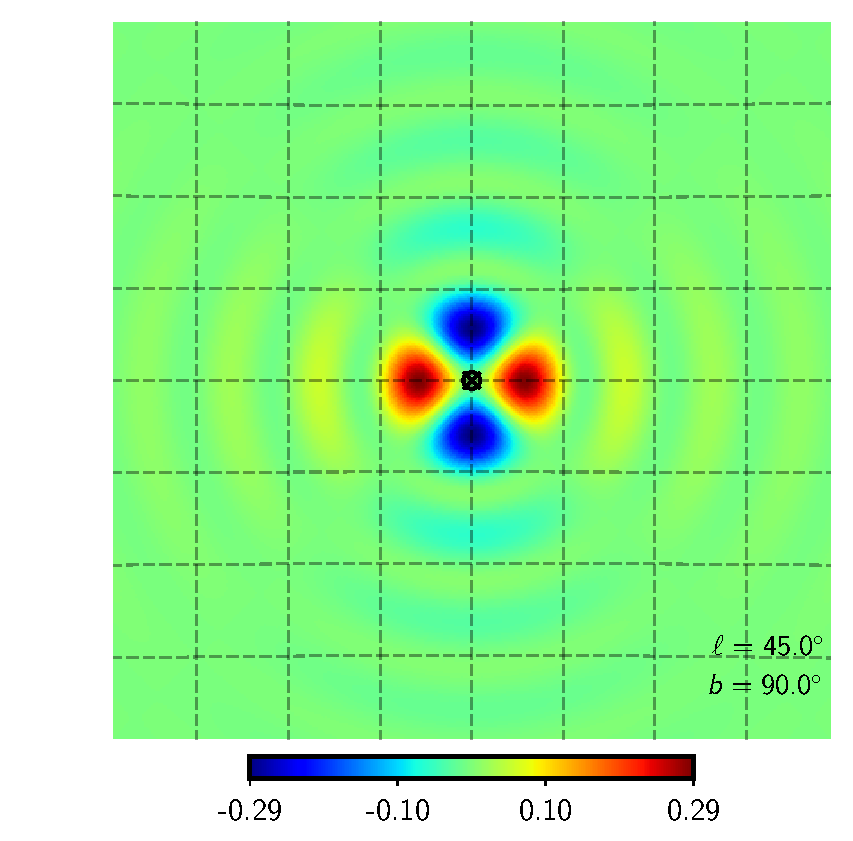
\includegraphics[width=0.125\columnwidth]{new_kernel/qu2eb_rker_rad_lat90_lon45.pdf}}\hspace{-2mm}
\subfigure{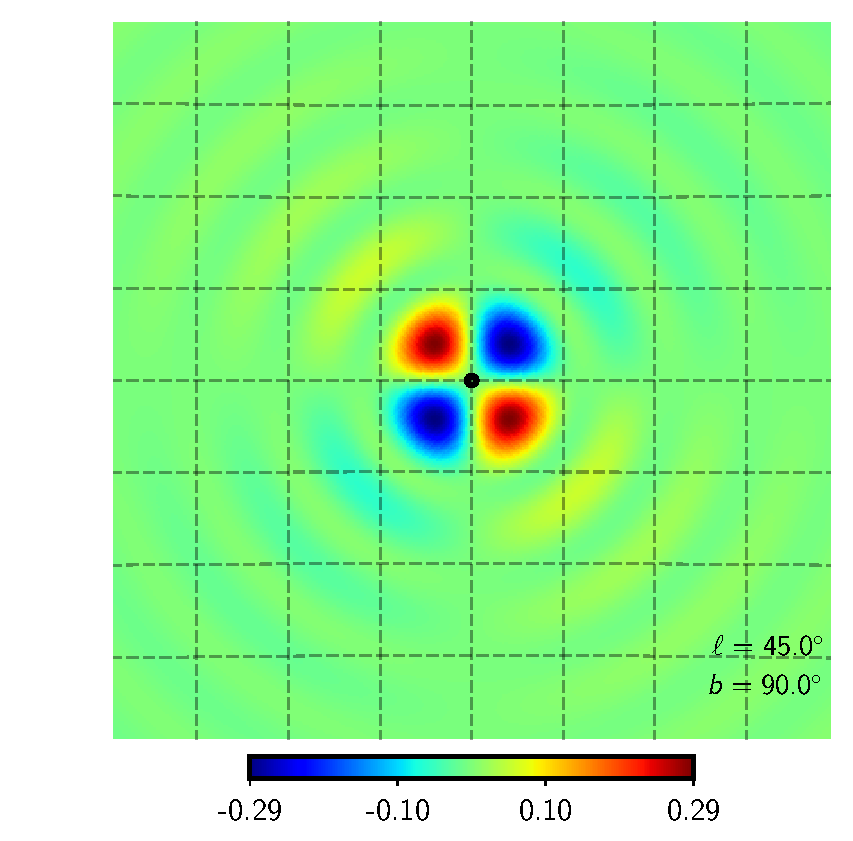
\includegraphics[width=0.125\columnwidth]{new_kernel/qu2eb_iker_rad_lat90_lon45.pdf}}\hspace{-2mm}
\subfigure{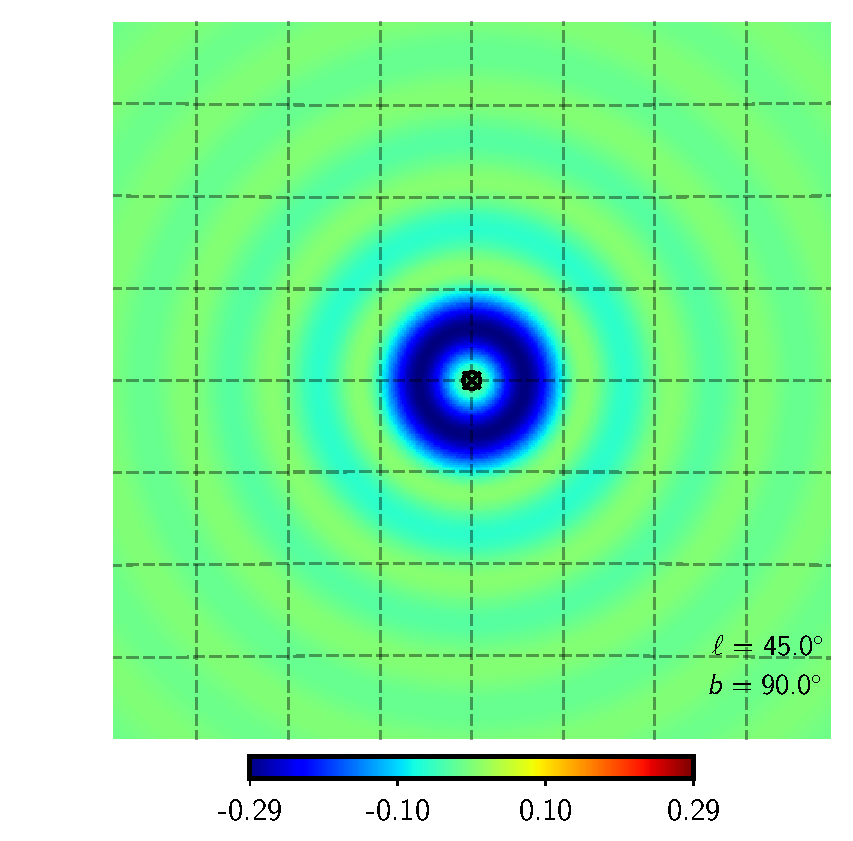
\includegraphics[width=0.125\columnwidth]{new_kernel/qu2eb_rker_con_lat90_lon45.pdf}}\hspace{-2mm}
\subfigure{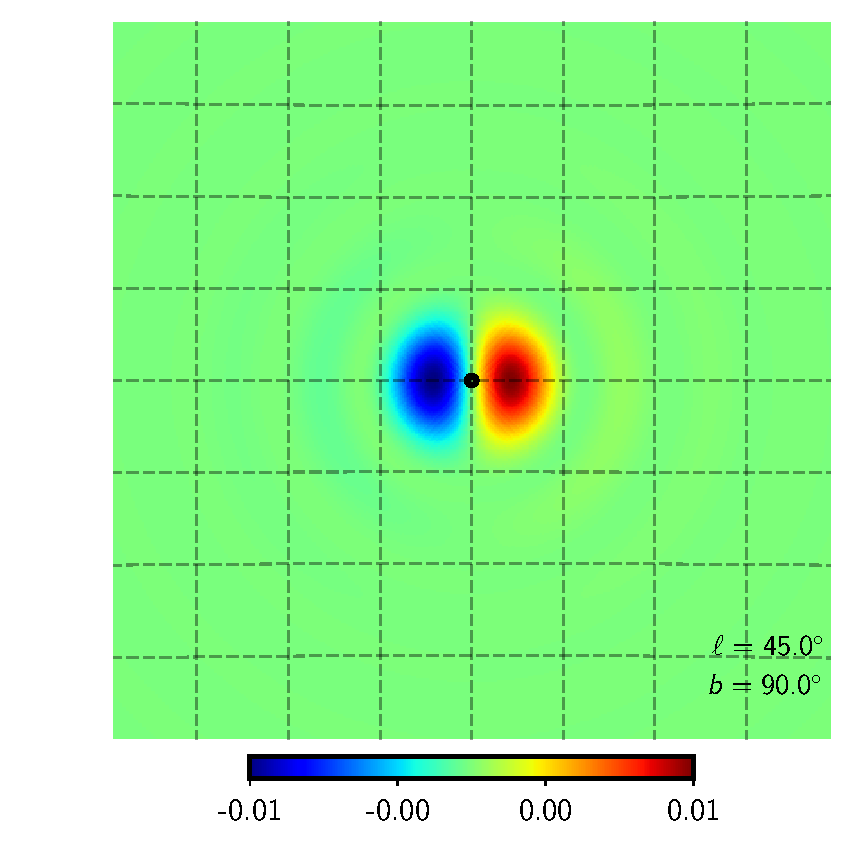
\includegraphics[width=0.125\columnwidth]{new_kernel/qu2eb_iker_con_lat90_lon45.pdf}}\hspace{-2mm}
\subfigure{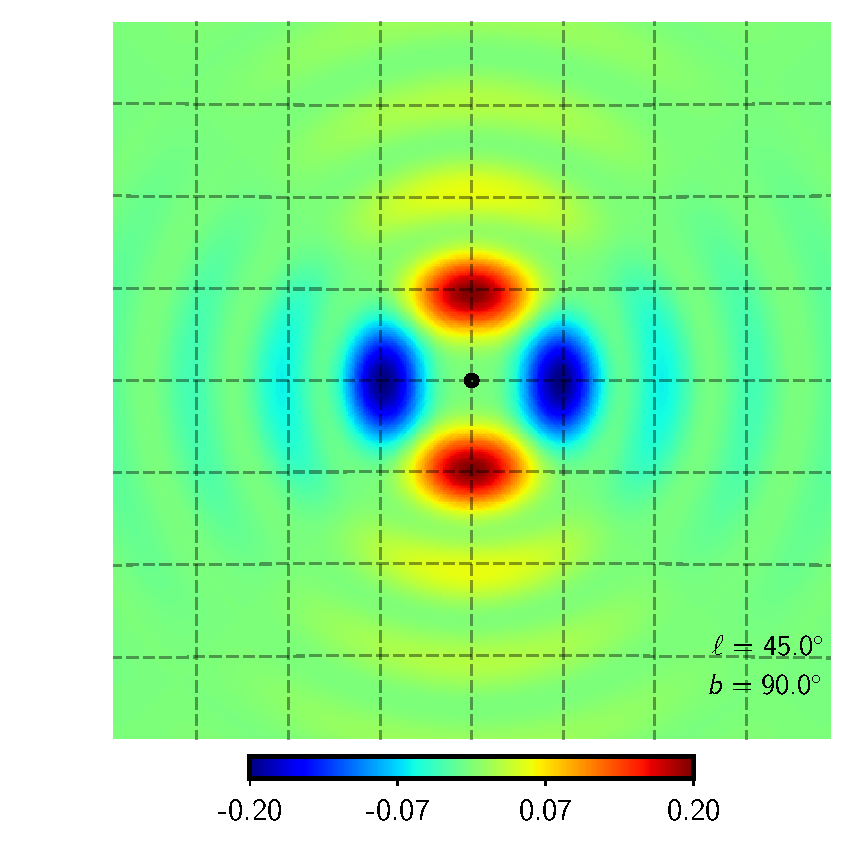
\includegraphics[width=0.125\columnwidth]{new_kernel/qu2ebqu_rker_D_lat90_lon45.pdf}}\hspace{-2mm}
\subfigure{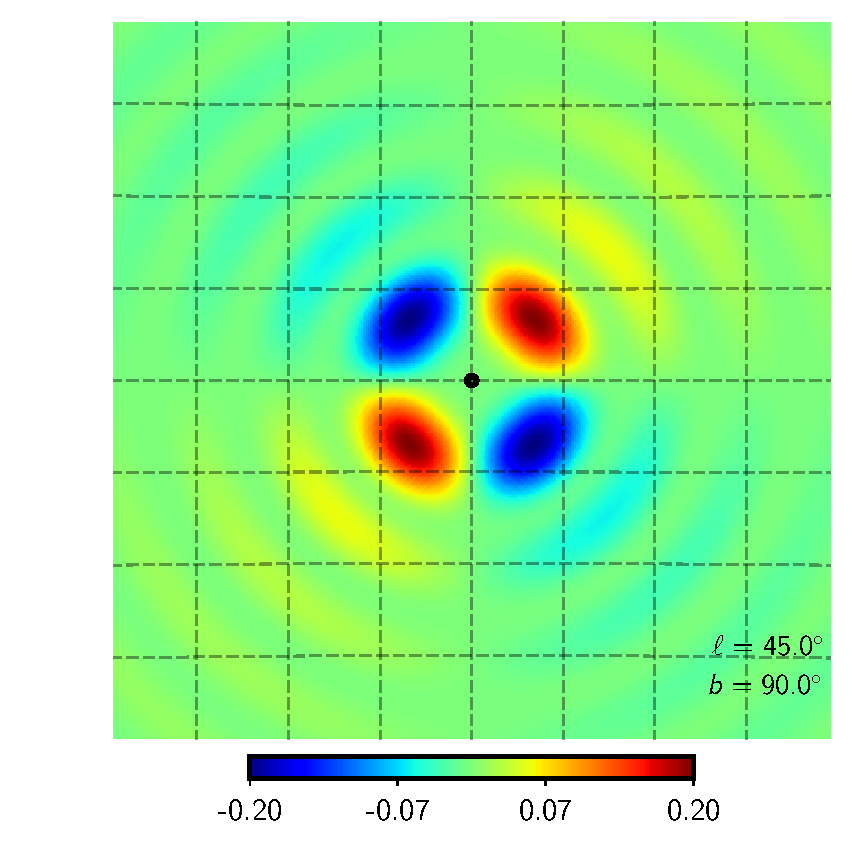
\includegraphics[width=0.125\columnwidth]{new_kernel/qu2ebqu_iker_D_lat90_lon45.pdf}}\hspace{-2mm}
\subfigure{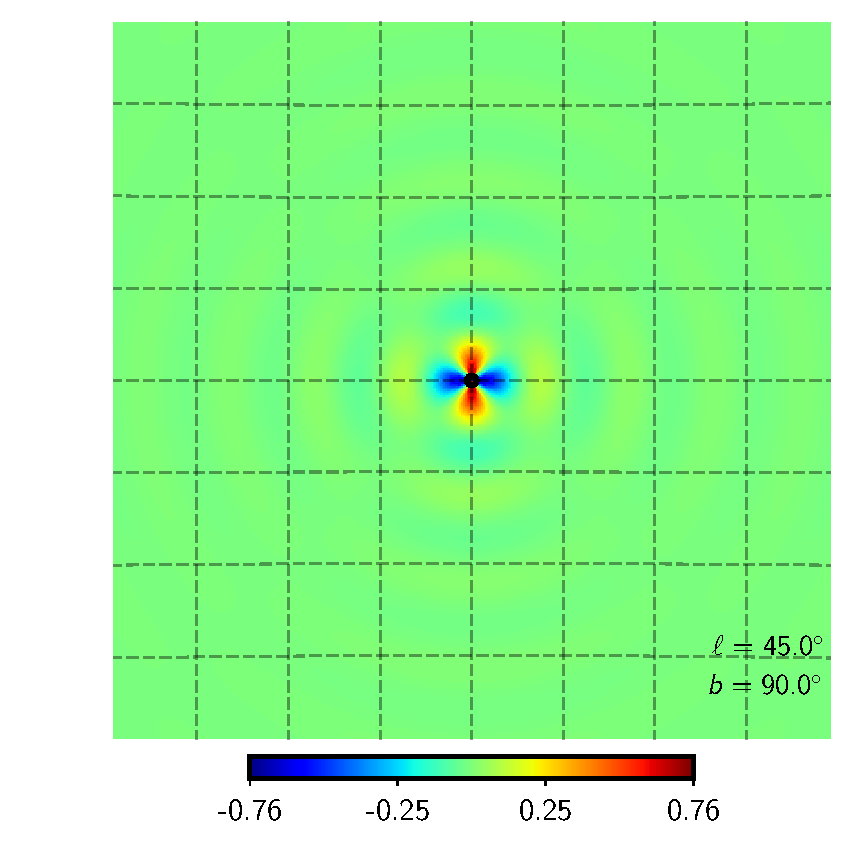
\includegraphics[width=0.125\columnwidth]{new_kernel/qu2ebqu_rker_I_lat90_lon45.pdf}}\hspace{-2mm}
\subfigure{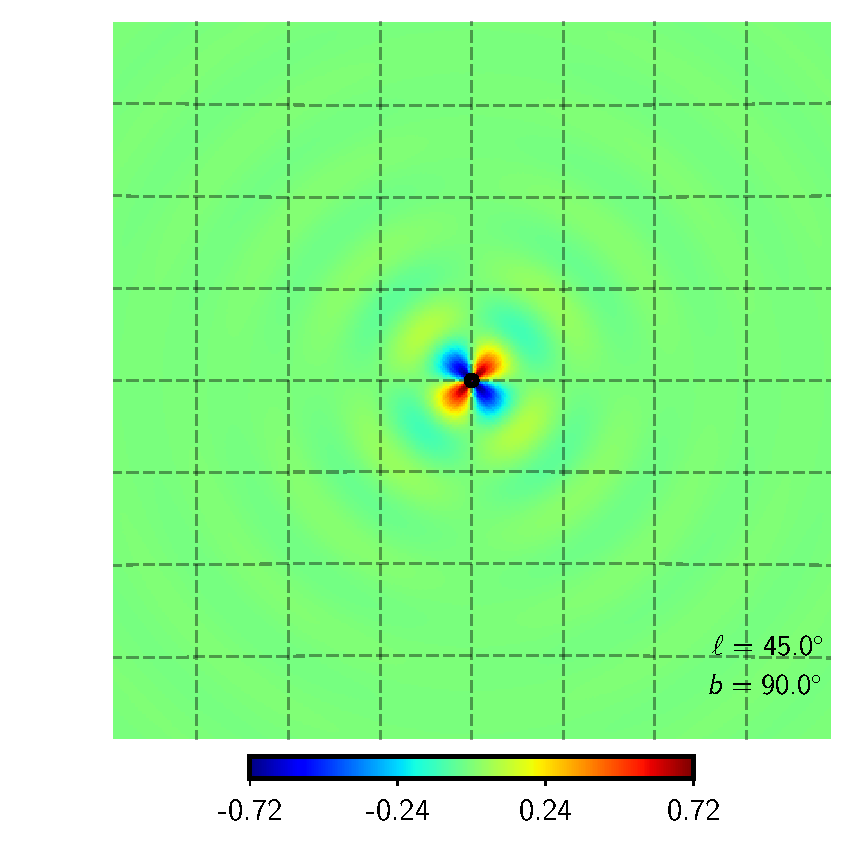
\includegraphics[width=0.125\columnwidth]{new_kernel/qu2ebqu_iker_I_lat90_lon45.pdf}}\hspace{-2mm}

\subfigure{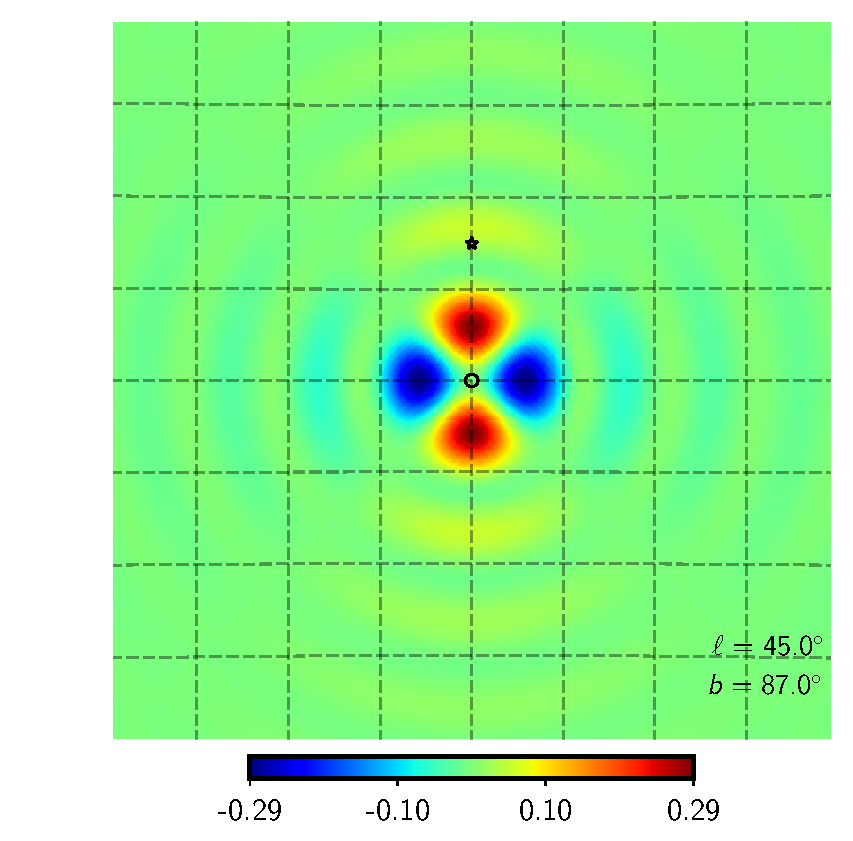
\includegraphics[width=0.125\columnwidth]{new_kernel/qu2eb_rker_rad_lat87_lon45.pdf}}\hspace{-2mm}
\subfigure{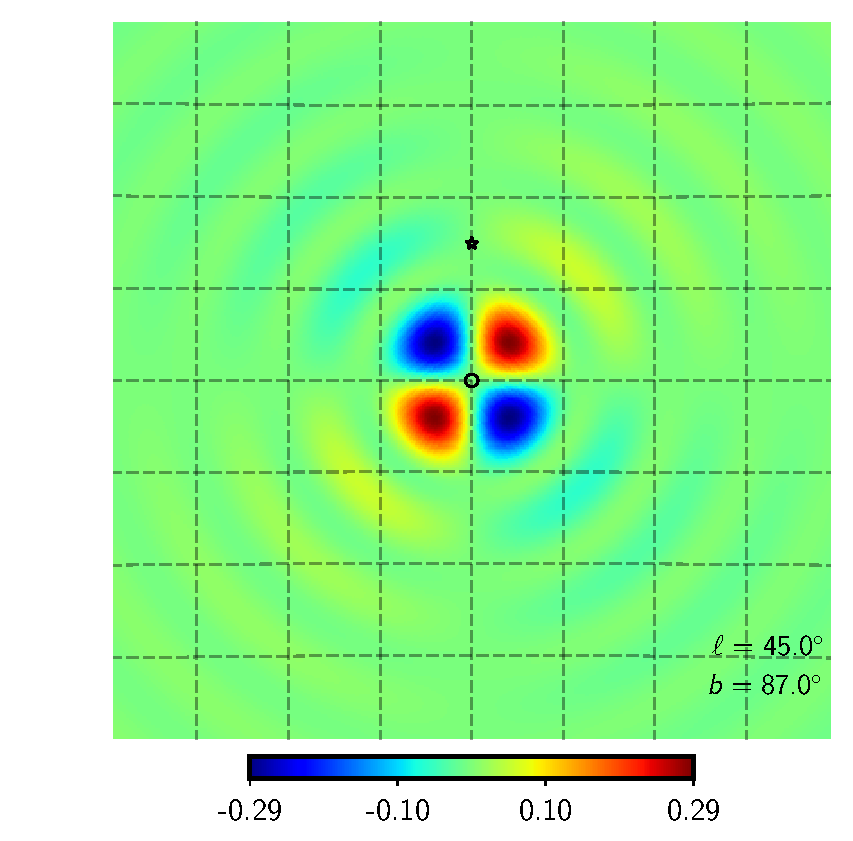
\includegraphics[width=0.125\columnwidth]{new_kernel/qu2eb_iker_rad_lat87_lon45.pdf}}\hspace{-2mm}
\subfigure{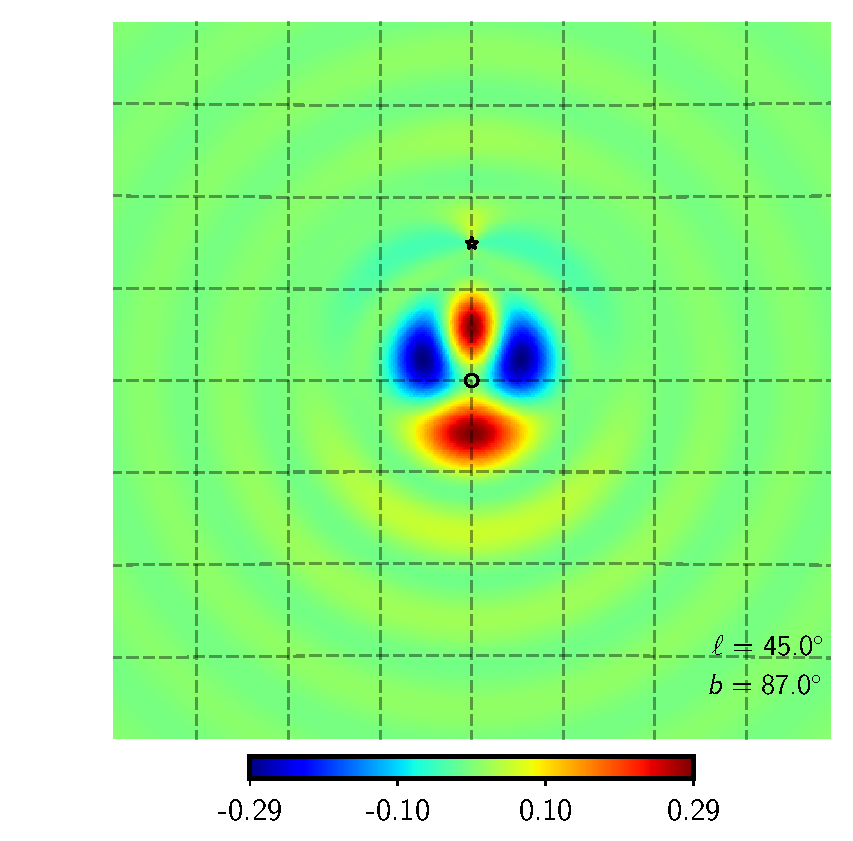
\includegraphics[width=0.125\columnwidth]{new_kernel/qu2eb_rker_con_lat87_lon45.pdf}}\hspace{-2mm}
\subfigure{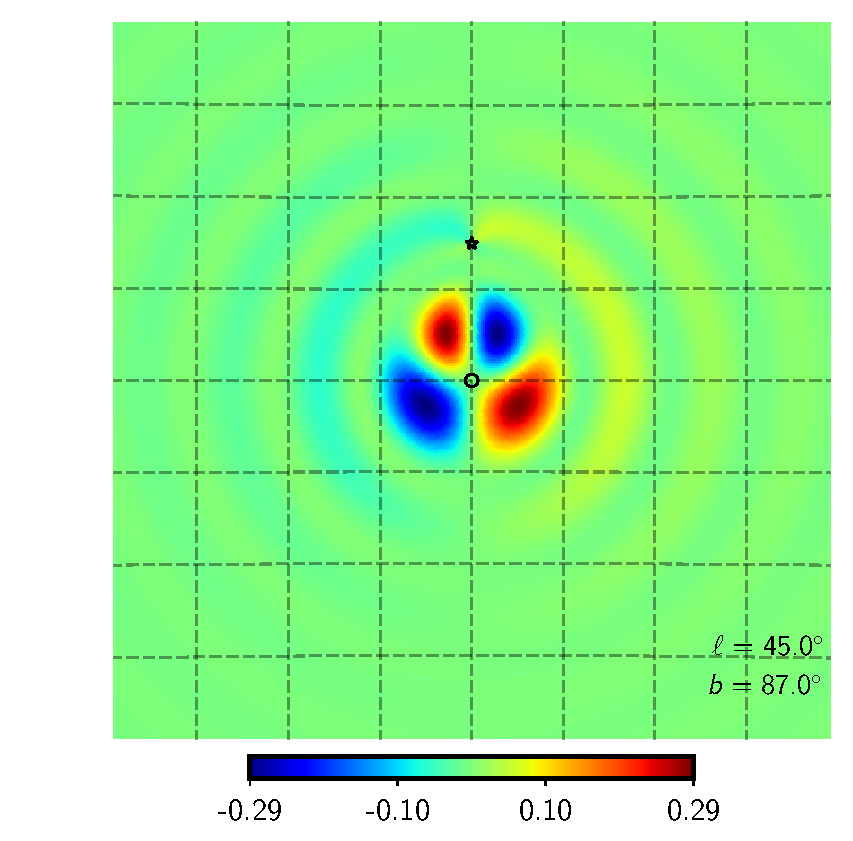
\includegraphics[width=0.125\columnwidth]{new_kernel/qu2eb_iker_con_lat87_lon45.pdf}}\hspace{-2mm}
\subfigure{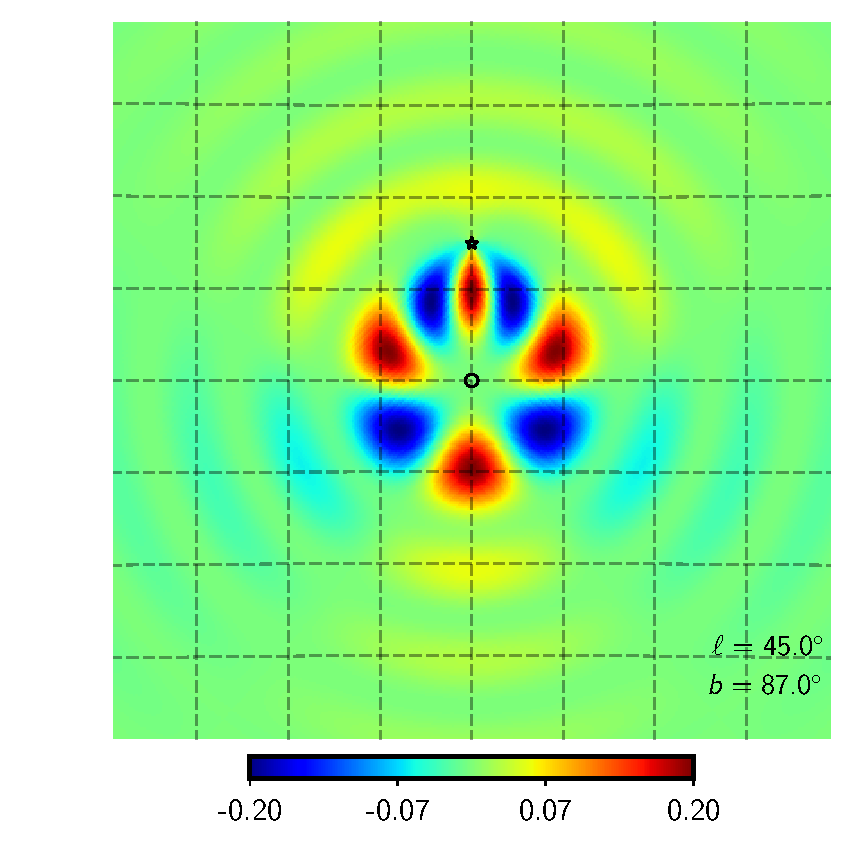
\includegraphics[width=0.125\columnwidth]{new_kernel/qu2ebqu_rker_D_lat87_lon45.pdf}}\hspace{-2mm}
\subfigure{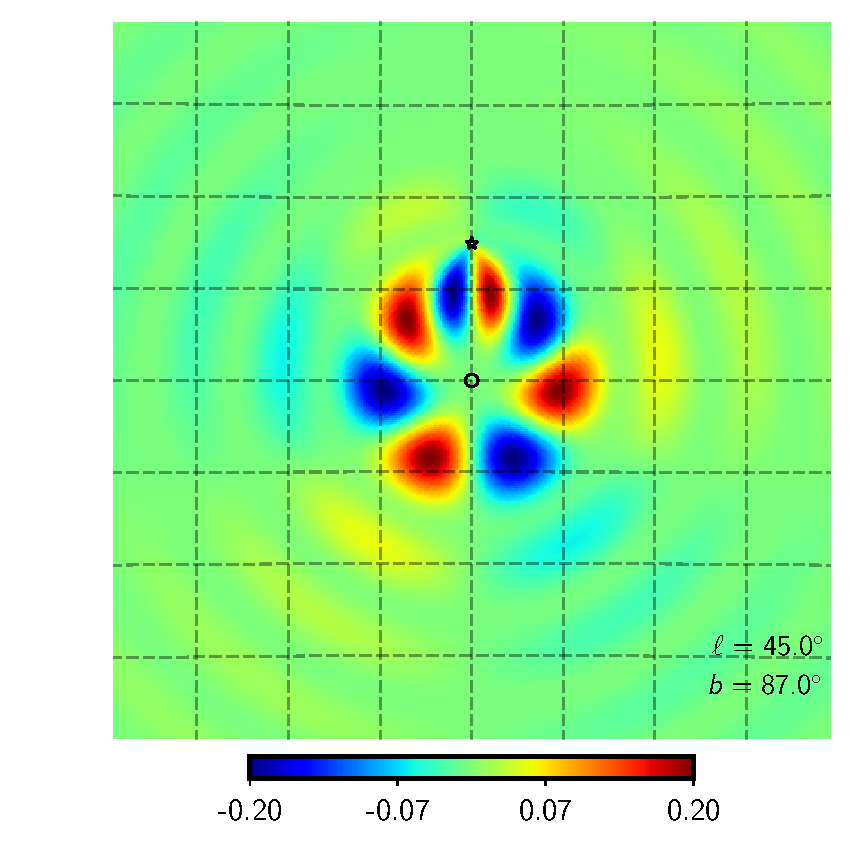
\includegraphics[width=0.125\columnwidth]{new_kernel/qu2ebqu_iker_D_lat87_lon45.pdf}}\hspace{-2mm}
\subfigure{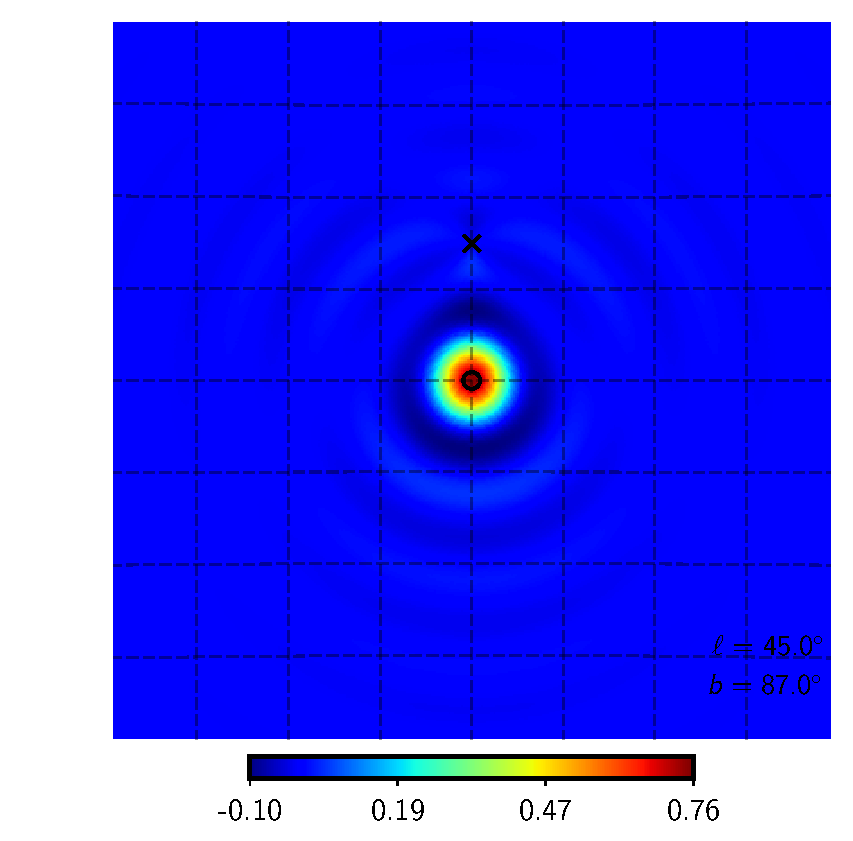
\includegraphics[width=0.125\columnwidth]{new_kernel/qu2ebqu_rker_I_lat87_lon45.pdf}}\hspace{-2mm}
\subfigure{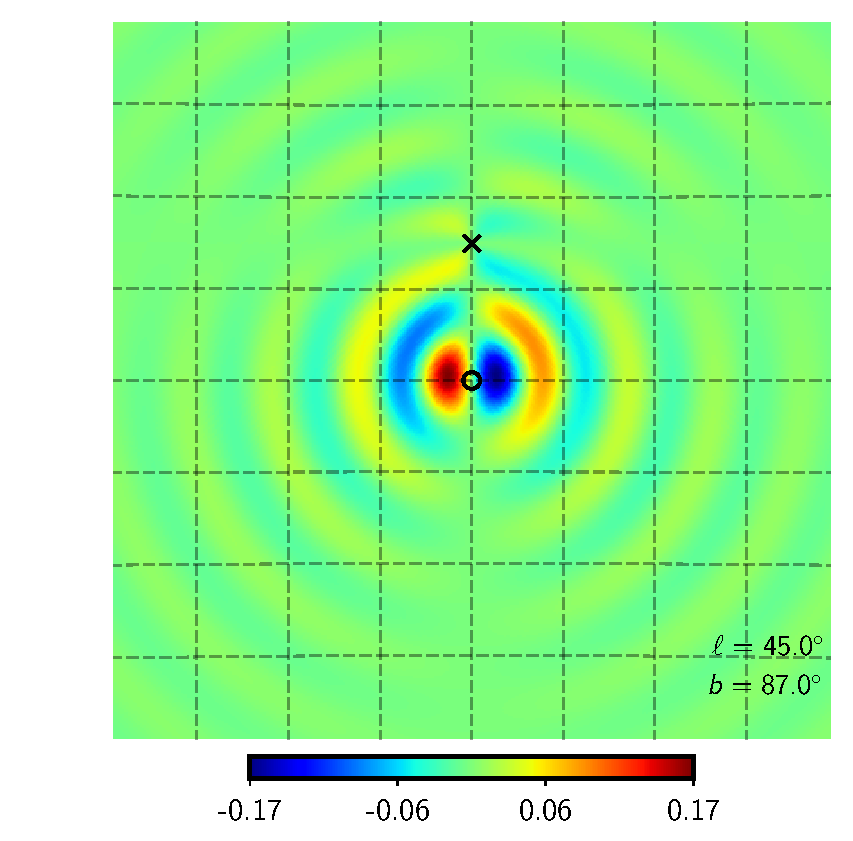
\includegraphics[width=0.125\columnwidth]{new_kernel/qu2ebqu_iker_I_lat87_lon45.pdf}}\hspace{-2mm}

\subfigure{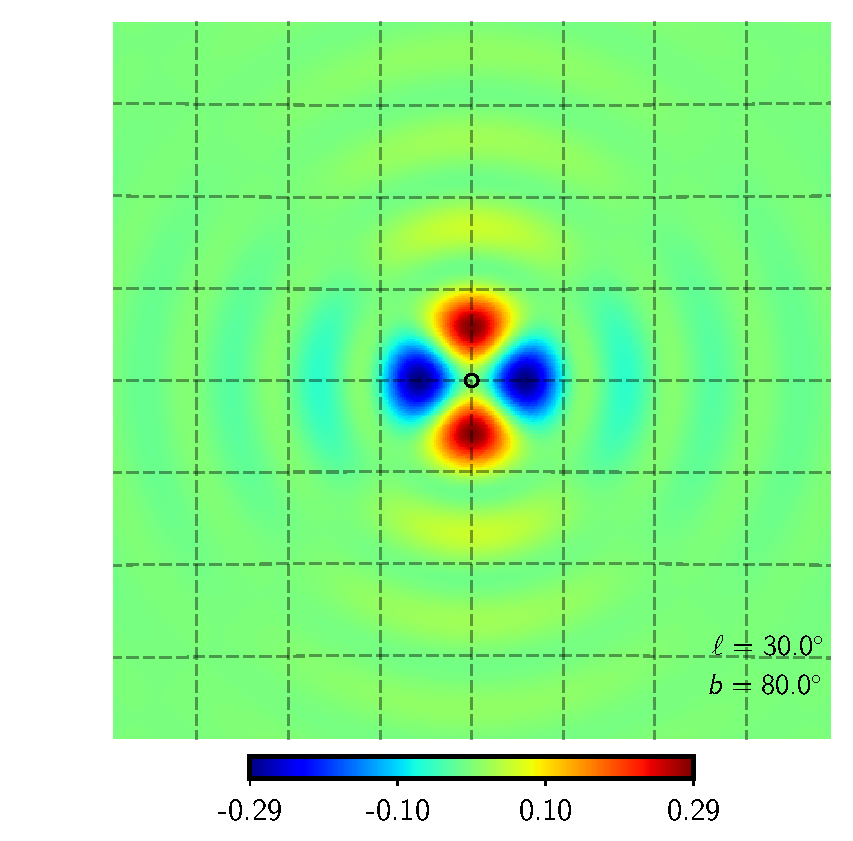
\includegraphics[width=0.125\columnwidth]{new_kernel/qu2eb_rker_rad_lat80_lon30.pdf}}\hspace{-2mm}
\subfigure{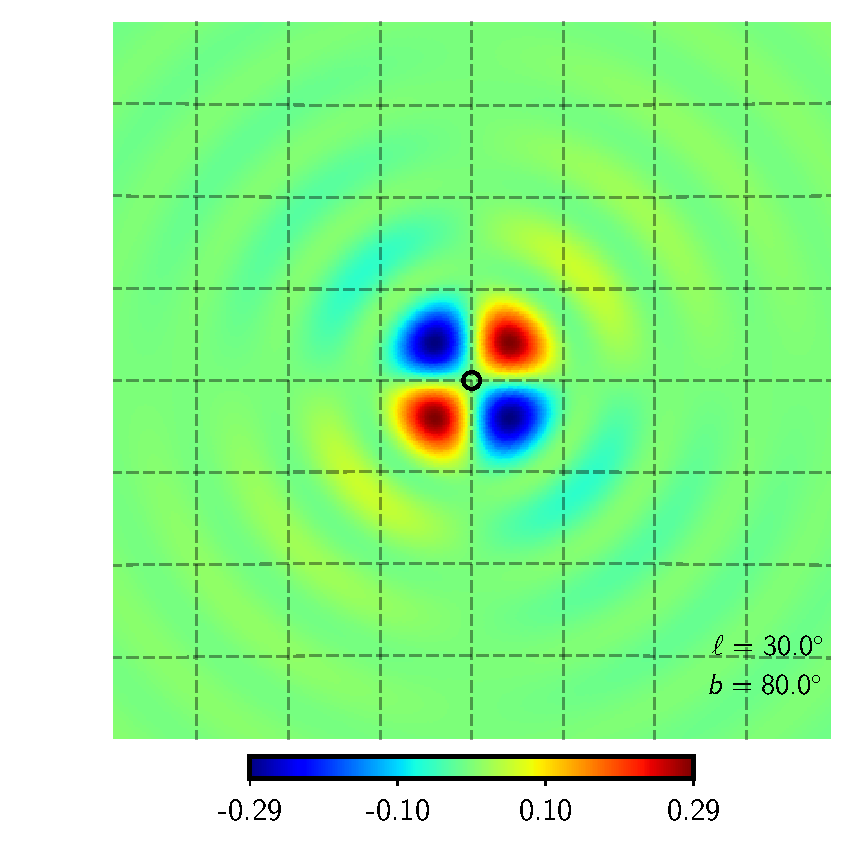
\includegraphics[width=0.125\columnwidth]{new_kernel/qu2eb_iker_rad_lat80_lon30.pdf}}\hspace{-2mm}
\subfigure{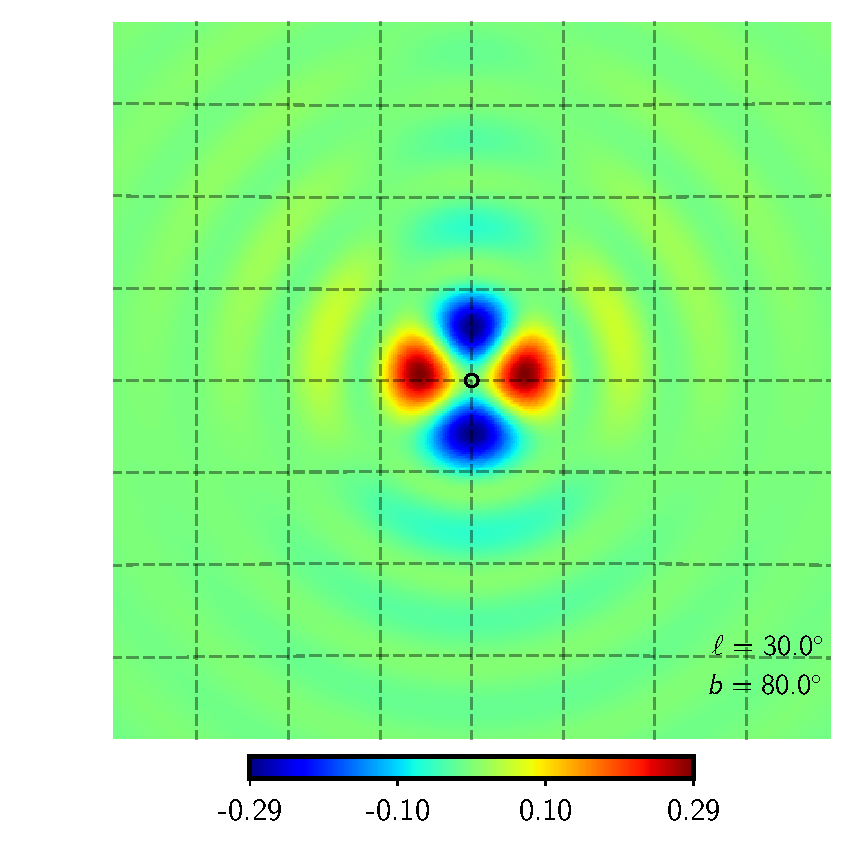
\includegraphics[width=0.125\columnwidth]{new_kernel/qu2eb_rker_con_lat80_lon30.pdf}}\hspace{-2mm}
\subfigure{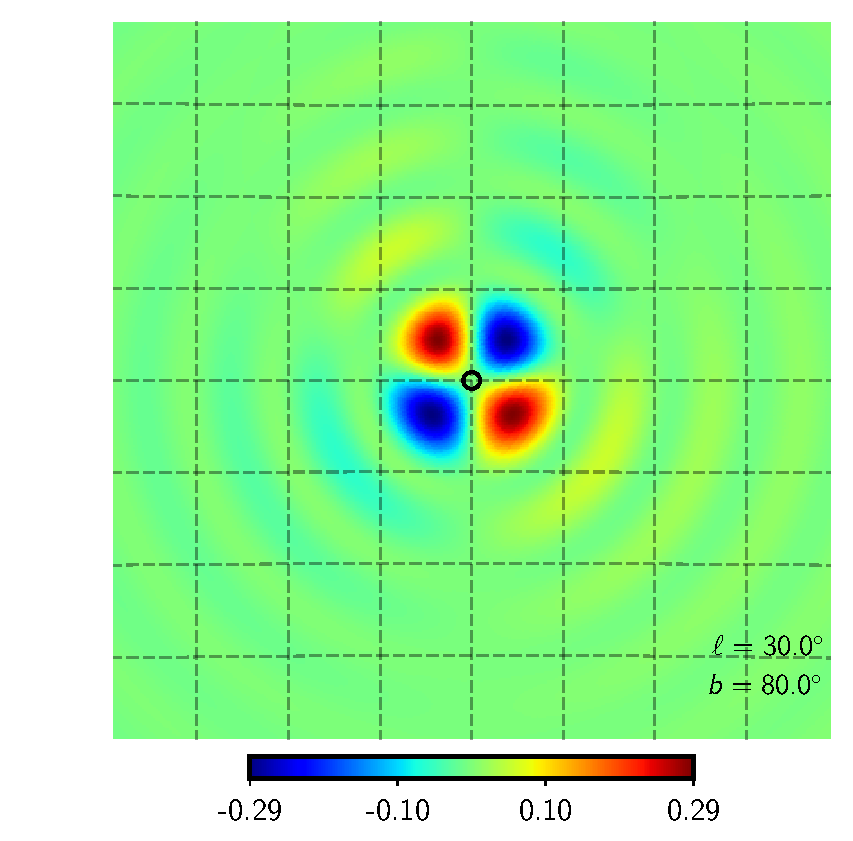
\includegraphics[width=0.125\columnwidth]{new_kernel/qu2eb_iker_con_lat80_lon30.pdf}}\hspace{-2mm}
\subfigure{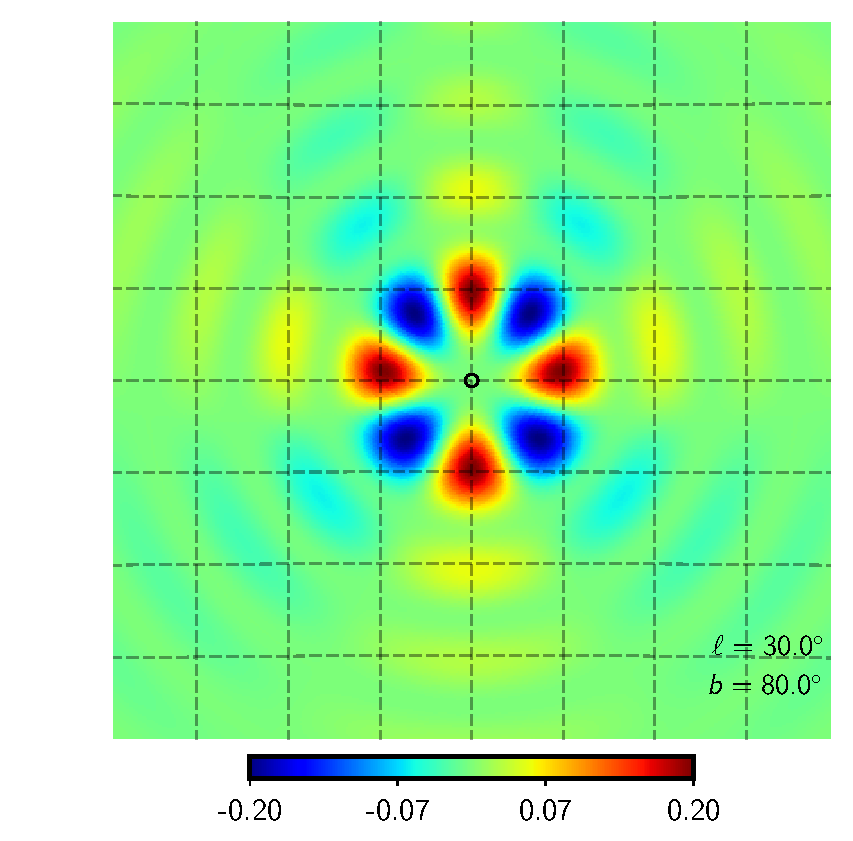
\includegraphics[width=0.125\columnwidth]{new_kernel/qu2ebqu_rker_D_lat80_lon30.pdf}}\hspace{-2mm}
\subfigure{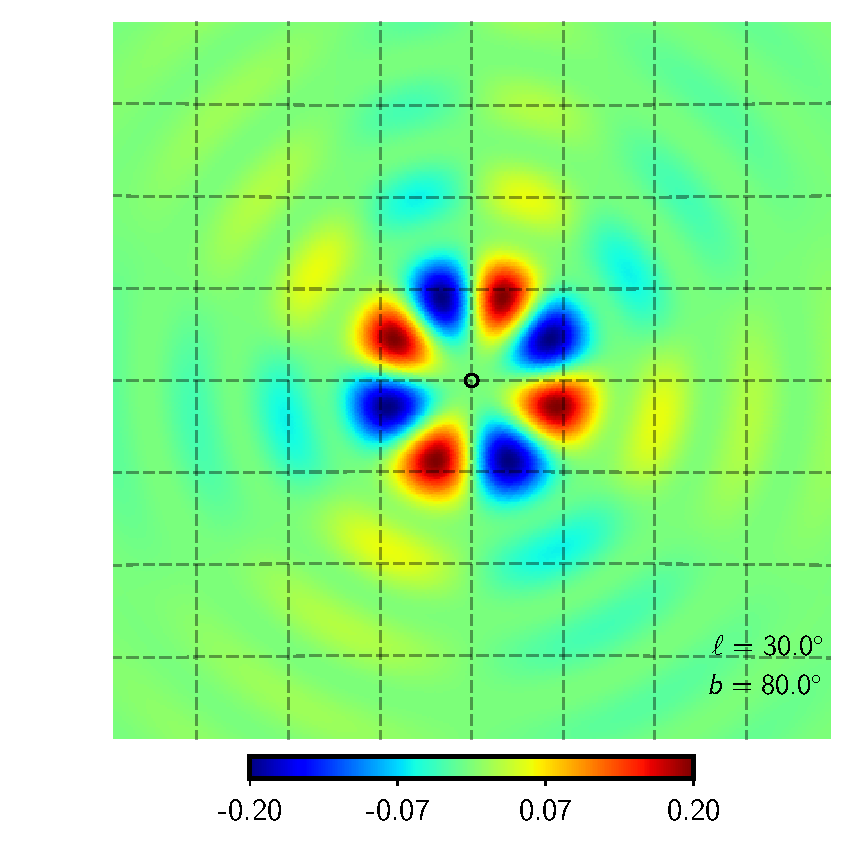
\includegraphics[width=0.125\columnwidth]{new_kernel/qu2ebqu_iker_D_lat80_lon30.pdf}}\hspace{-2mm}
\subfigure{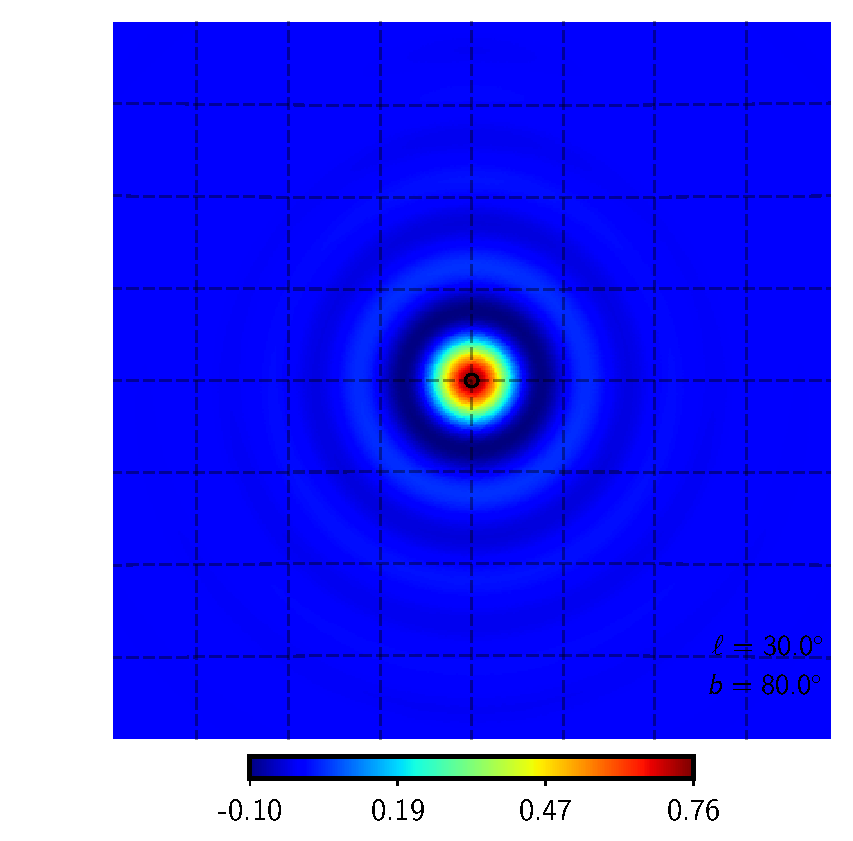
\includegraphics[width=0.125\columnwidth]{new_kernel/qu2ebqu_rker_I_lat80_lon30.pdf}}\hspace{-2mm}
\subfigure{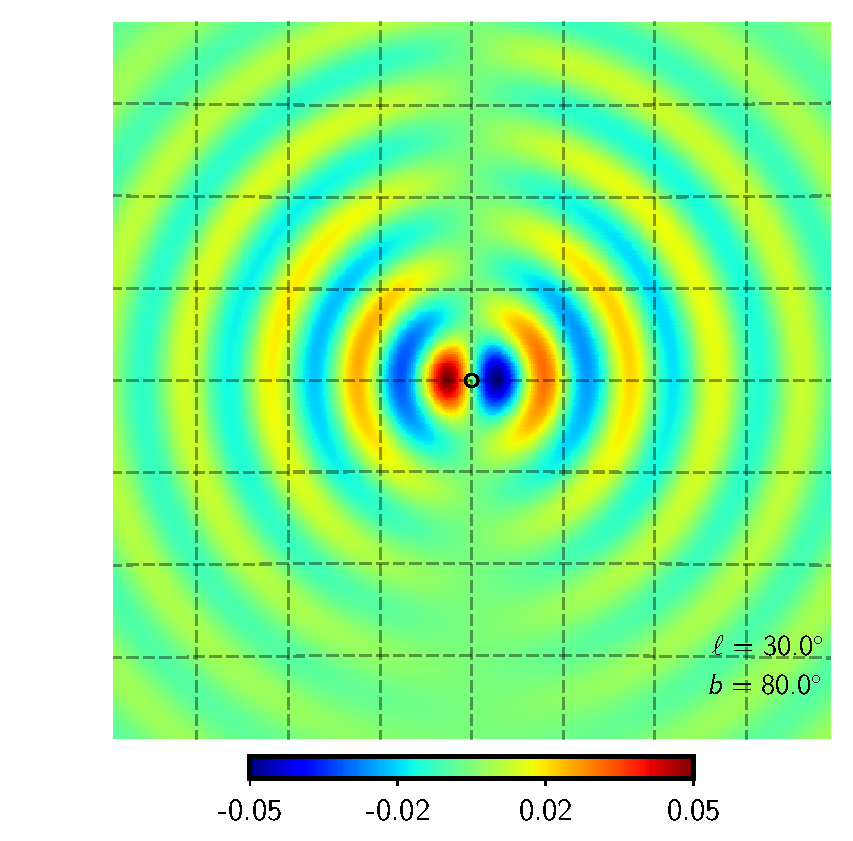
\includegraphics[width=0.125\columnwidth]{new_kernel/qu2ebqu_iker_I_lat80_lon30.pdf}}\hspace{-2mm}
\subfigure[$ \textrm{Re} \left(\mathcal{M}_{G} \right) $]{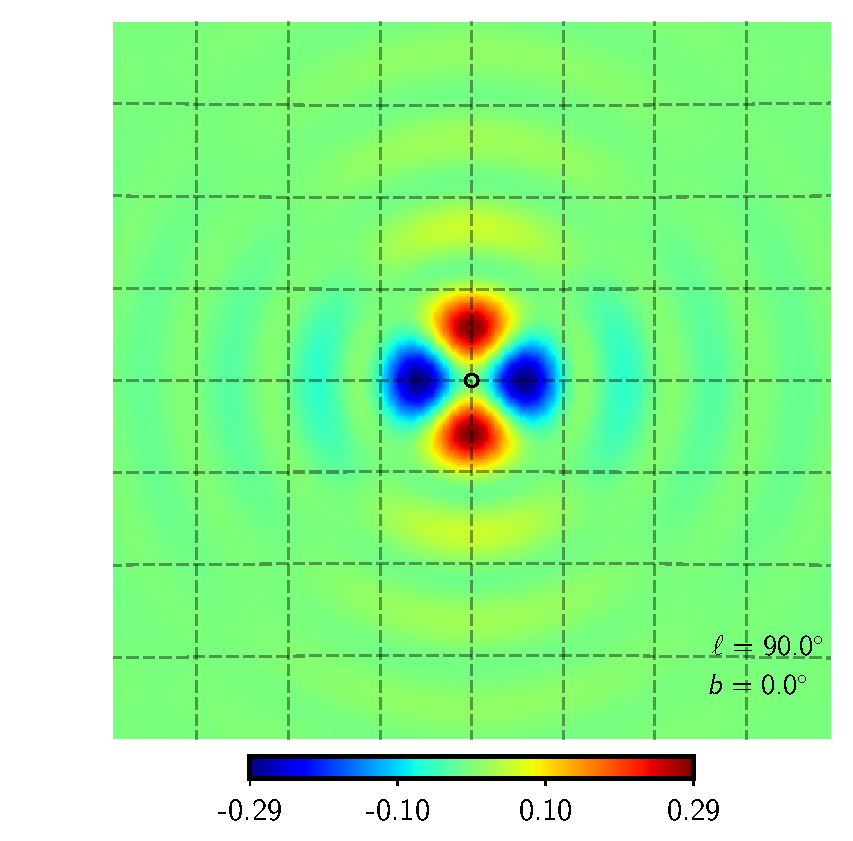
\includegraphics[width=0.125\columnwidth]{new_kernel/qu2eb_rker_rad_lat0_lon90.pdf}}\hspace{-2mm}
\subfigure[$\textrm{Img} \left(\mathcal{M}_{G} \right) $]{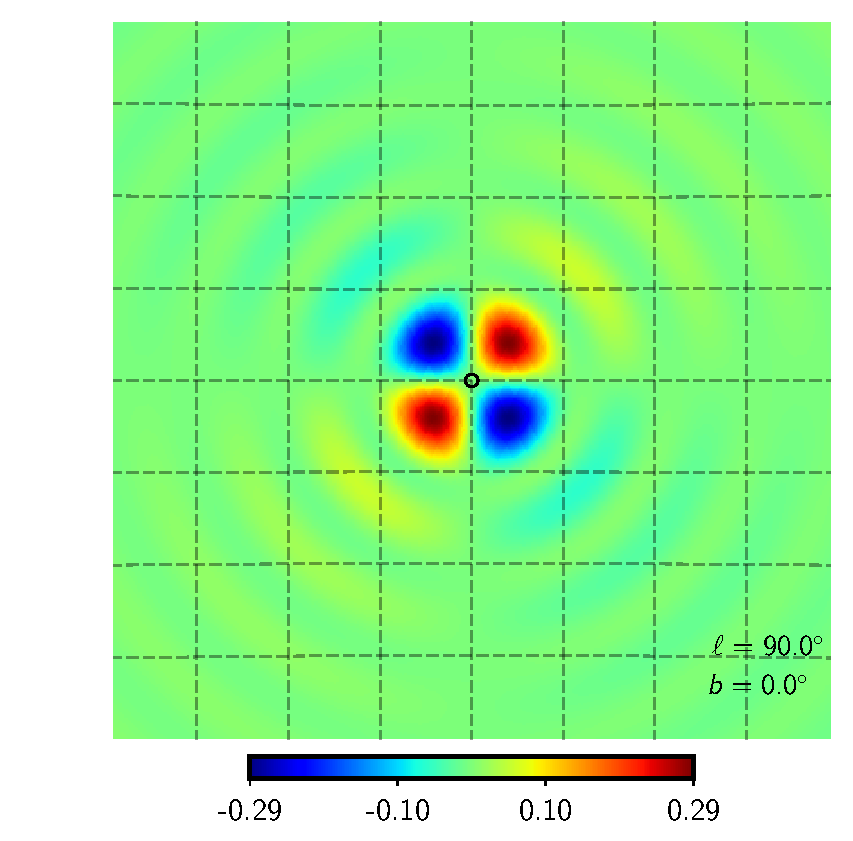
\includegraphics[width=0.125\columnwidth]{new_kernel/qu2eb_iker_rad_lat0_lon90.pdf}}\hspace{-2mm}
\subfigure[$\textrm{Re}  \left(\mathcal{M}_{B} \right) $]{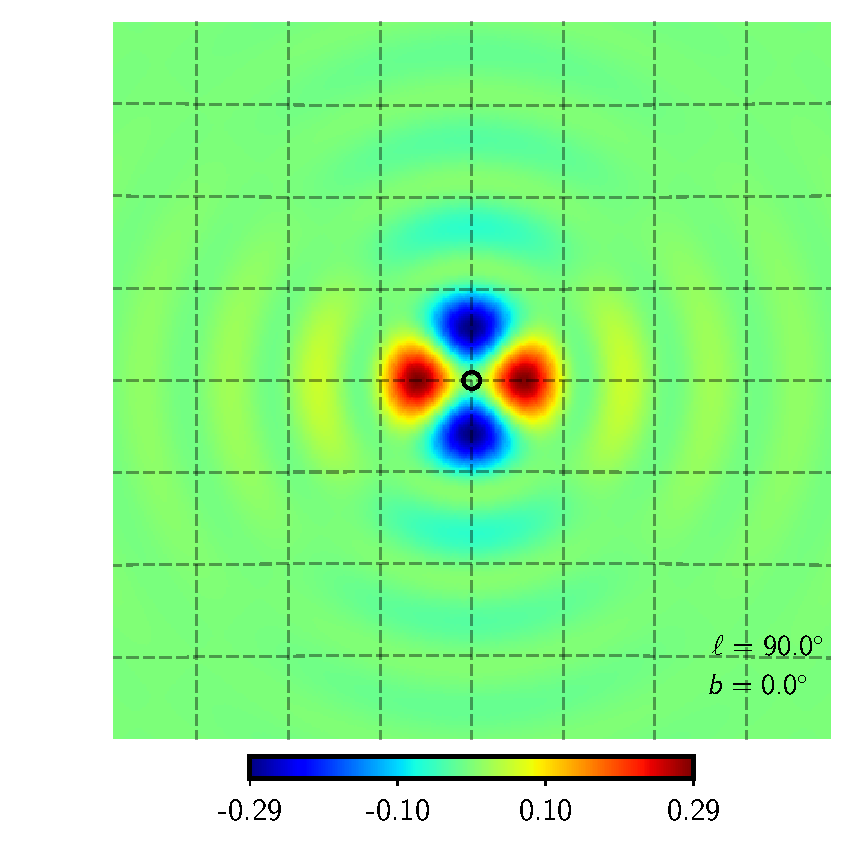
\includegraphics[width=0.125\columnwidth]{new_kernel/qu2eb_rker_con_lat0_lon90.pdf}}\hspace{-2mm}
\subfigure[$\textrm{Img} \left(\mathcal{M}_{B} \right) $]{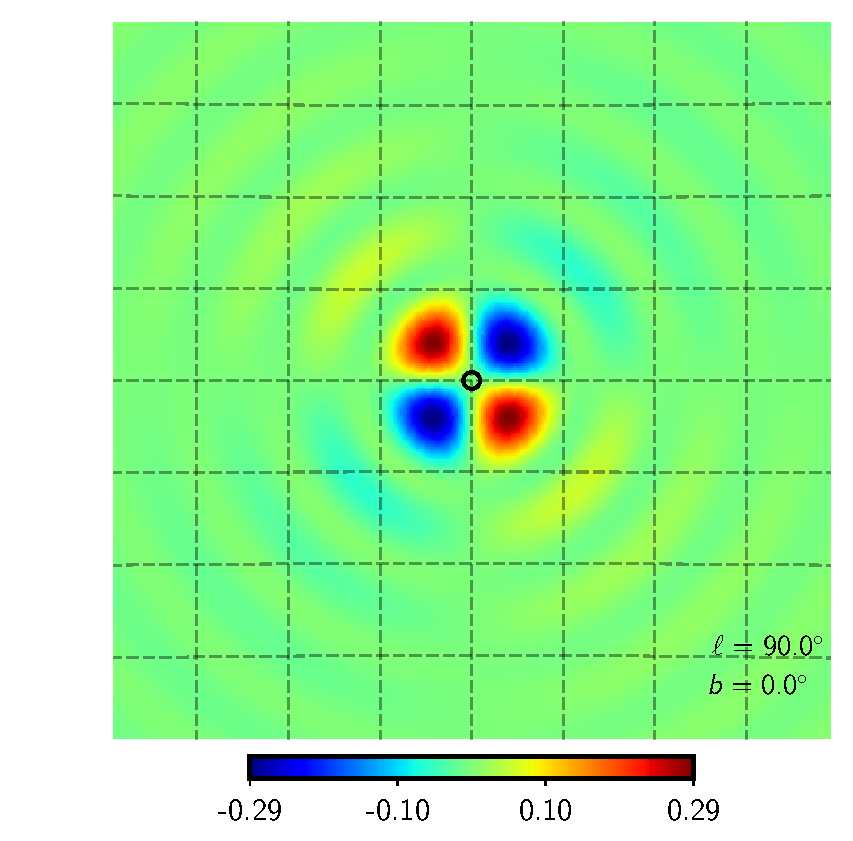
\includegraphics[width=0.125\columnwidth]{new_kernel/qu2eb_iker_con_lat0_lon90.pdf}}\hspace{-2mm}
\subfigure[$\textrm{Re} \left(\mathcal{D} \right)$]{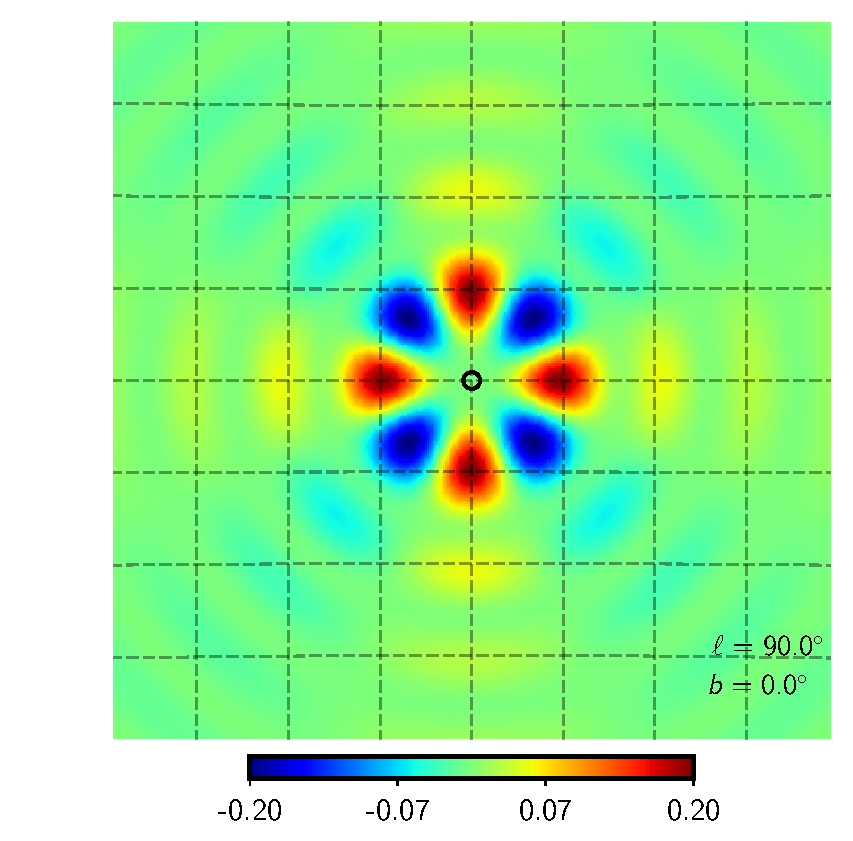
\includegraphics[width=0.125\columnwidth]{new_kernel/qu2ebqu_rker_D_lat0_lon90.pdf}}\hspace{-2mm}
\subfigure[$\textrm{Img} \left(\mathcal{D} \right)$]{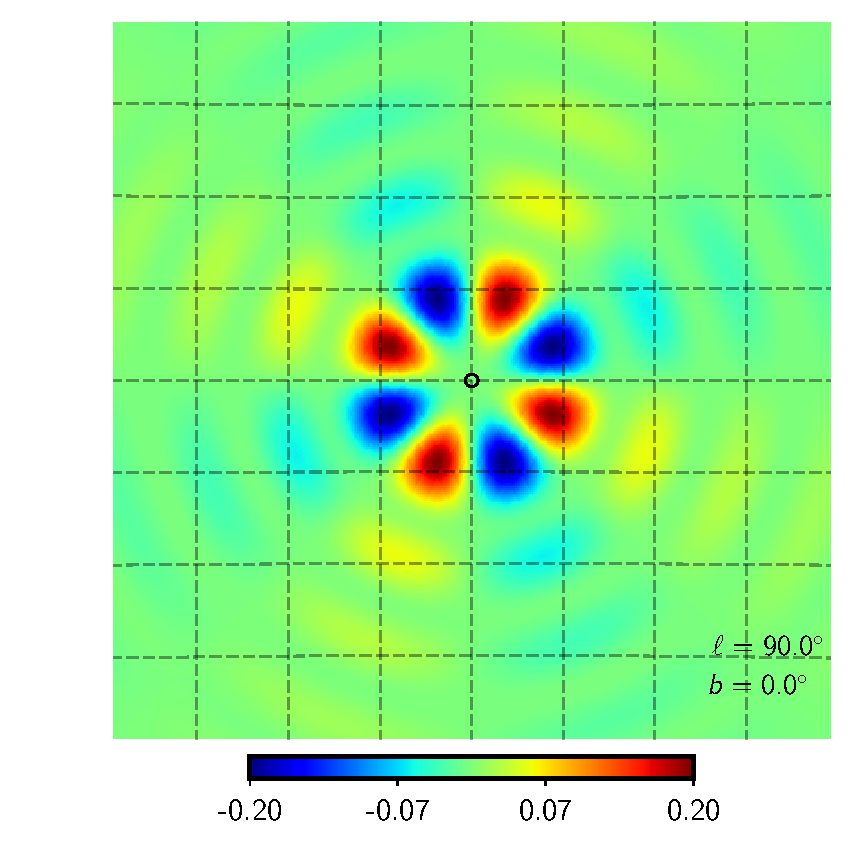
\includegraphics[width=0.125\columnwidth]{new_kernel/qu2ebqu_iker_D_lat0_lon90.pdf}}\hspace{-2mm}
\subfigure[$\textrm{Re} \left(\mathcal{I} \right)$]{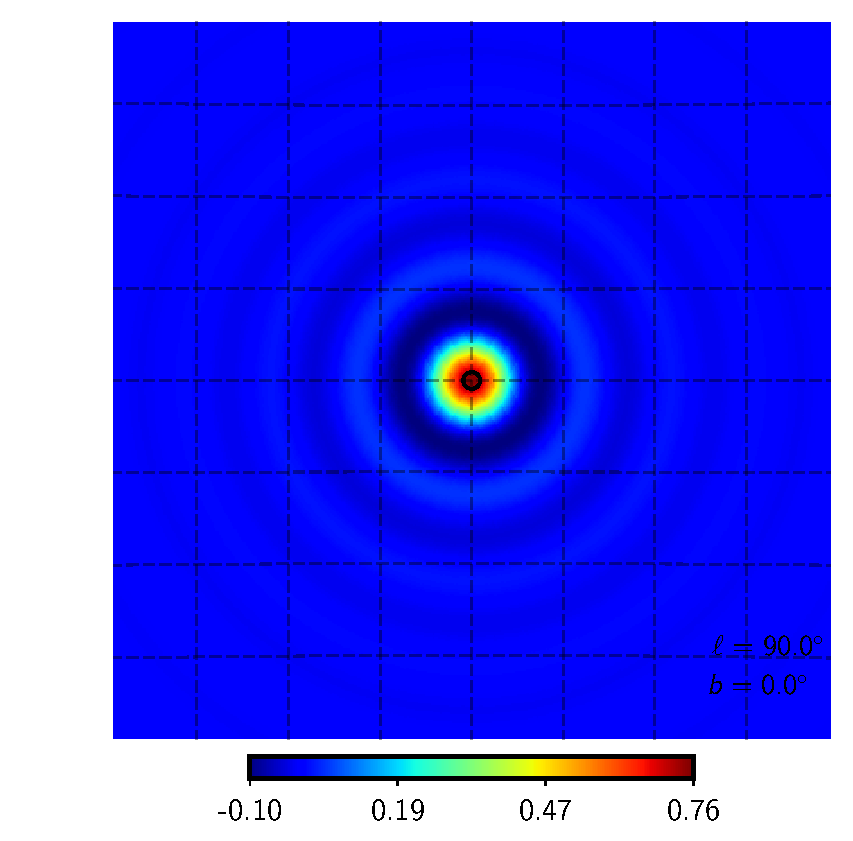
\includegraphics[width=0.125\columnwidth]{new_kernel/qu2ebqu_rker_I_lat0_lon90.pdf}}\hspace{-2mm}
\subfigure[$\textrm{Img} \left(\mathcal{I} \right)$]{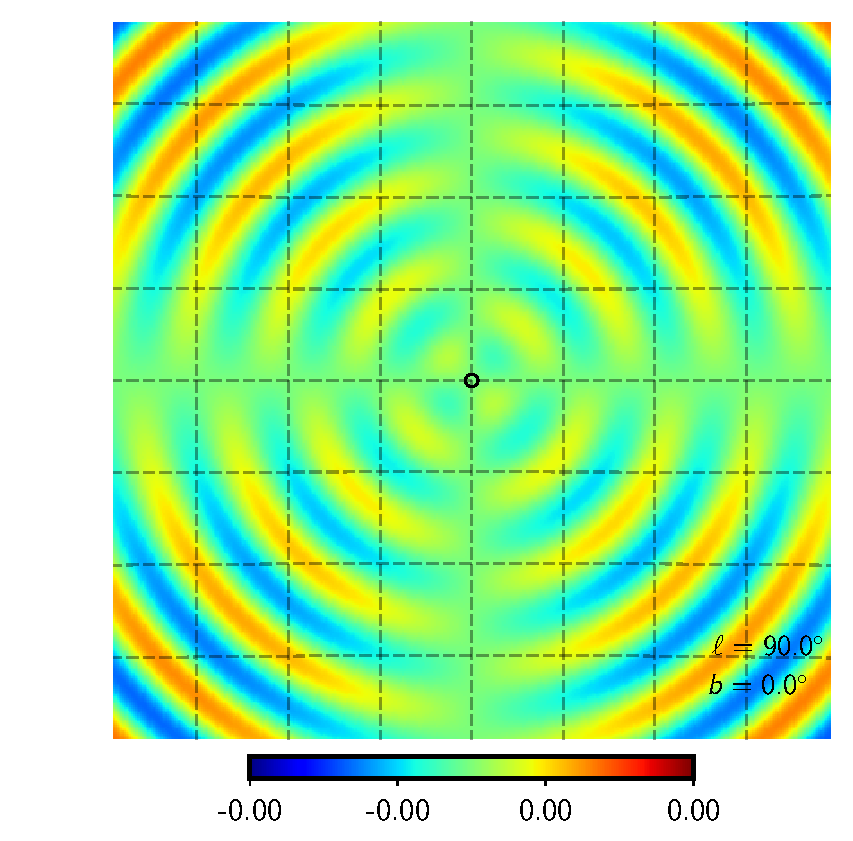
\includegraphics[width=0.125\columnwidth]{new_kernel/qu2ebqu_iker_I_lat0_lon90.pdf}}\hspace{-2mm}
\caption{This panel of figure depicts the real and imaginary parts of the real space kernels $\mathcal{M}_{G}$, $\mathcal{M}_{B}$, $\mathcal{D}$ \& $\mathcal{I}$ respectively. These kernels have been evaluated with the band limit: $\ell \in [2,192]$ and sampled at the Healpix resolution parameter NSIDE=2048 for visual appeal. The size of each panel is approximately $16^{\circ} \times 16^{\circ}$ and the grid lines are marked at 2 degree separations. The black circles denotes the position of the center around which the kernels have been evaluated while the black star marks the location of the north galactic pole. The four rows depict the kernels at different location on the sphere and the galactic coordinates of the central pixel are specified in each panel.}
%from top to bottom rows are as follows $[b,\ell] = [0^{\circ},0^{\circ}], [87^{\circ},0^{\circ}], [87^{\circ},30^{\circ}], [80^{\circ},30^{\circ}], [0^{\circ},90^{\circ}]$.}
\label{fig:vis_kernel}
 \end{figure}
%

%\textit{Evaluating the local kernels: }\revisit{Let us consider the case when one of the coordinates coincides with the north pole $\hat{z}=(0,0)$ (this refers to the point $\theta_0 \rightarrow 0$ while moving along the longitude $\phi_0=0$). In this case the Euler angles in the $z-y1-z2$ convention are simply given by: $(\alpha,\beta,\gamma) =(\phi_i,\theta_i,0)$, where $(\theta_i,\phi_i)$ denote the coordinates of the location $\hat{n}_i$.} Since the Euler angle $\gamma=0$ when rotations are defined with respect to the pole, the respective kernels simplify to the following forms,
%%
%\begin{subequations}
%\beqry 
%\mathcal{M}(\hat{z},\hat{n}_i) &=&  \sum_{\ell} {{}_{0}}a_{\ell 2} \, {{}_{0}}Y_{\ell 2}(\hat{n}_i) \,;\\
%\mathcal{I}(\hat{z},\hat{n}_i) &=& \sum_{\ell} {{}_{-2}}a_{\ell 2}\, {{}_{-2}}Y_{\ell 2}(\hat{n}_i) ~~\,;~~
%\mathcal{D}(\hat{z},\hat{n}_i) =\sum_{\ell} {{}_{2}}a_{\ell 2} \, {{}_{2}}Y_{\ell 2}(\hat{n}_i) \,,
%\eeqry
%\end{subequations}
%%
%where ${}_{s}a_{\ell 2} = \sqrt{\frac{2 \ell+1}{ 4 \pi}} ~~\forall ~~ s \in [0,-2,+2]$.
%The convolution kernels centered around any other location $\hat{n}_j = (\theta_j,\phi_j)$ are simply given by evaluating the respective spherical harmonic sums: $\sum_{\ell m} {}_{s}a_{\ell m}\,{}_{s}Y_{\ell m}(\hat{n}_i)$ using the rotated harmonic coefficients given by: ${}_s a_{\ell m} = D^{\ell}_{m 2}(\phi_j , \theta_j, 0) {{}_s}a_{\ell 2}$, where $D^{\ell}_{2 m}$ are the Wigner-D functions.
%These rotation operations can be carried out using inbuilt Healpix routine \textit{rotate\_alm}, while the convolution kernels can be synthesized by evaluating the respective spherical harmonic sums using the \textit{alm2map} routine. 
%\comment{Make parallels with instrument beam analysis here ? Or is it trivial since its obvious that all convolution problems can be cast in this form.}

We compute the Euler angles $(\alpha, \beta, \gamma)$ given the angular coordinates of any two Healpix pixels and use these to evaluate the convolution and the radiating kernels. To provide an intuition for how these kernels vary as a function of position of the central pixel we depict in \fig{fig:vis_kernel} the respective kernels at a few different locations on the sphere.
While the kernels are evaluated in the band limit $\ell \in [2,192]$, for illustration these functions are sampled at a very high Healpix resolution parameter of NSIDE=2048. All the plots have been rotated such that the central location marked by the black circle are in the centre of the figure. The horizontal and vertical lines that pass through the central black circle mark the local latitude and longitude respectively.

The real and imaginary part of the kernel $\mathcal{M}_G$ are identical irrespective of changes in the galactic latitude and longitude of the central pixel. This is consistent with the Green's function interpretation of these kernels. Note that these functions are not distorted when a part of the domain overlaps with the poles, as can be seen in the first three rows of \fig{fig:vis_kernel}. Both these facts can be associated with the fact that this function does not depend on the Euler angle $\gamma$. From \eq{eq:qu2eb_convolution_explicit} and \eq{eq:eb2qu_convolution_explicit} it is clear that $\mathcal{M}_r$ and $\mathcal{M}_i$ can be interpreted in the following ways,
%\revisit{Recall that the angle $\gamma$ defines the rotation about the final z-axis which co-alligns the planar axes. Since the function $\mathcal{M}$ does not depend of this final orientation, it implies a rotational invariance of the fields constructed by convolving with this kernel.}
%
\begin{subequations}
\beqry
\bmat E= -\mathcal{M}_r \\ B =+\mathcal{M}_i  \emat  \leftarrow \bmat Q=\delta(\hat{n} - \hat{n}_j)\\ U=0 \emat ~~;~~ \bmat E= -\mathcal{M}_i \\ B = - \mathcal{M}_r  \emat  \leftarrow \bmat Q=0 \\ U=\delta(\hat{n} - \hat{n}_j) \emat \,,  \\
\bmat Q= -\mathcal{M}_r \\ U = -\mathcal{M}_i  \emat  \leftarrow \bmat E=\delta(\hat{n} - \hat{n}_j)\\ B=0 \emat ~~;~~ \bmat Q= +\mathcal{M}_i \\ U = - \mathcal{M}_r  \emat  \leftarrow \bmat E=0 \\ B=\delta(\hat{n} - \hat{n}_j) \emat \,.
\eeqry
\end{subequations}
%
The kernels $\mathcal{D}$ \& $\mathcal{I}$ vary significantly as a function of galactic latitude of the central pixel as seen in the last four columns of \fig{fig:vis_kernel}. These kernels show a two fold symmetry in the vicinity of the poles and this arises due to Euler angle $\gamma \approx 0$ here and therefore $e^{i2(\alpha \pm \gamma)} \approx e^{i2\alpha}$. Note that in this region, the azimuthal profile of the real and imaginary part of these kernels  is similar to $\mathcal{M}_r$ and $\mathcal{M}_i$ respectively.  This explains why the imaginary part of the band limited delta function $\mathcal{I}$ contributes just as much as the real part in these regions. On transiting to lower latitudes, $\mathcal{D}$ quickly transitions to having a four fold symmetry while $\mathcal{I}$ transitions to being dominated by the real part and behaves more like the conventional delta function. This transition can be most easily understood in the flat sky limit where $\gamma = -\alpha$ which leads to the resultant 4 fold symmetry seen for $\mathcal{D}$ owing to $e^{i2(\alpha - \gamma)} =e^{i4\alpha}$ and $\mathcal{I}$ being dominated by the real part owing to $e^{-i2(\alpha + \gamma)} =1 + i0$. Since the flat sky approximation has most validity in the proximity of the equator these limiting tendencies of the respective kernels are seen in the bottom row of \fig{fig:vis_kernel} which depict the kernels evaluated at the equator $b=0^{\circ}$. The middle two row depict the kernels evaluated at a latitudes of $b=87^{\circ}~\&~ 80^{\circ}$ and serve to indicate the rate of this transition. These kernels are invariant under changes in longitude of the central pixel, the latitude being held fixed, as one may have expected.

%%%%%%%%%%%%%%%%%%%%%%%%%%%%%%%%%%%%%%%%%%%%%%%%%%%%%%%%%%%%%%%%%%%%%%%%%%
%\subsection{Quantifying the non-locality of E \& B modes} \label{sec:radial_locality}
\subsection{The non-locality of the real space operators} \label{sec:radial_locality}
%
\begin{figure}[t]
\centering
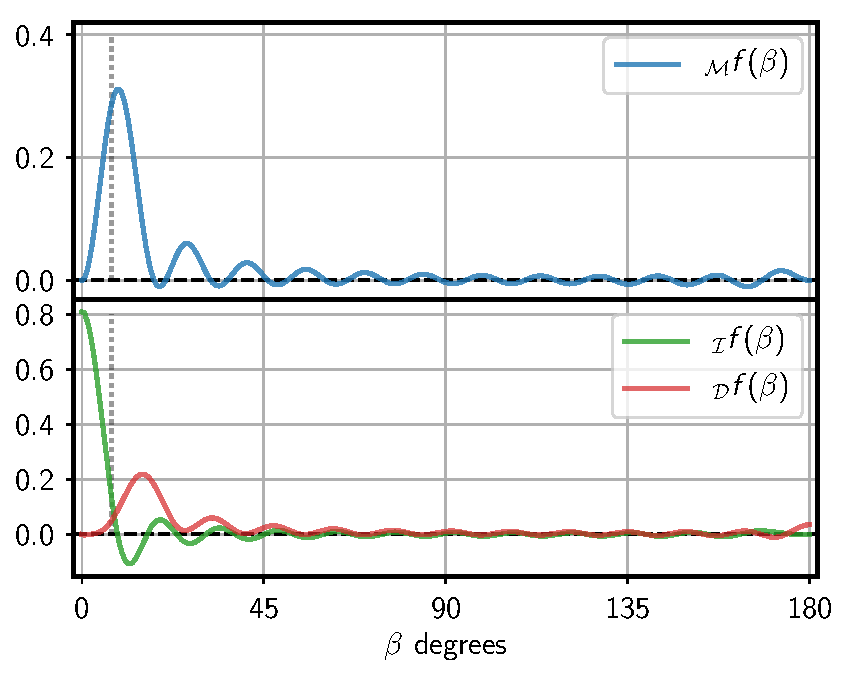
\includegraphics[width=0.8\columnwidth]{beta_kernel.pdf}
\caption{The figure depicts the radial part of the convolution kernels. These radial function have been evaluated with the band limit fixed at $\ell \in [2,24]$. The vertical dashed line marks the approximate Healpix pixel size of a NSIDE=8, which is the lowest resolution that allows access to $\ell_{\rm max}=24$.}
\label{fig:beta_kernel}
\end{figure}
%
In the previous section we presented a quantitative understanding of the  azimuthal dependence of the real space kernels, providing little insight into their radial dependence. The radial part of these kernels determines the non-locality of the respective operators and encodes all their multipole dependencies. For illustration the radial kernels ${_{\mm}f}, {_{\md}f} ~\&~ {_{\mi}f} $ are evaluated using the respective multipole sums given in \eq{eq:rad_ker_queb} and \eq{eq:f2_rad_ker} in the band limit $\ell \in [2,192]$ and the resultant functions are depicted in \fig{fig:beta_kernel}. 
%
\begin{figure}[t]
\centering
\subfigure{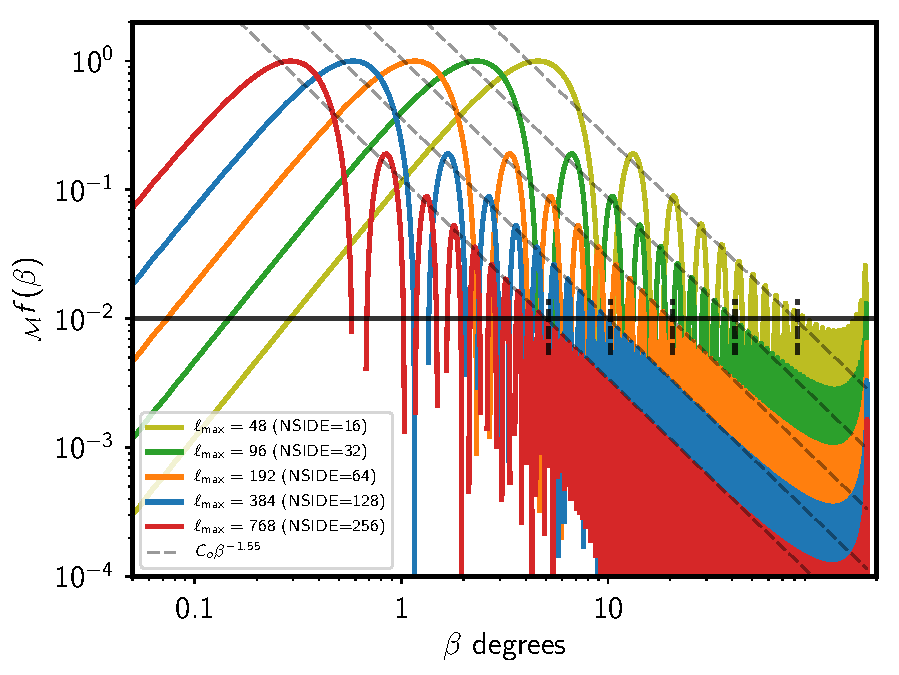
\includegraphics[width=0.96\columnwidth]{rad_ker_fn_of_ellmax.pdf}}
\subfigure{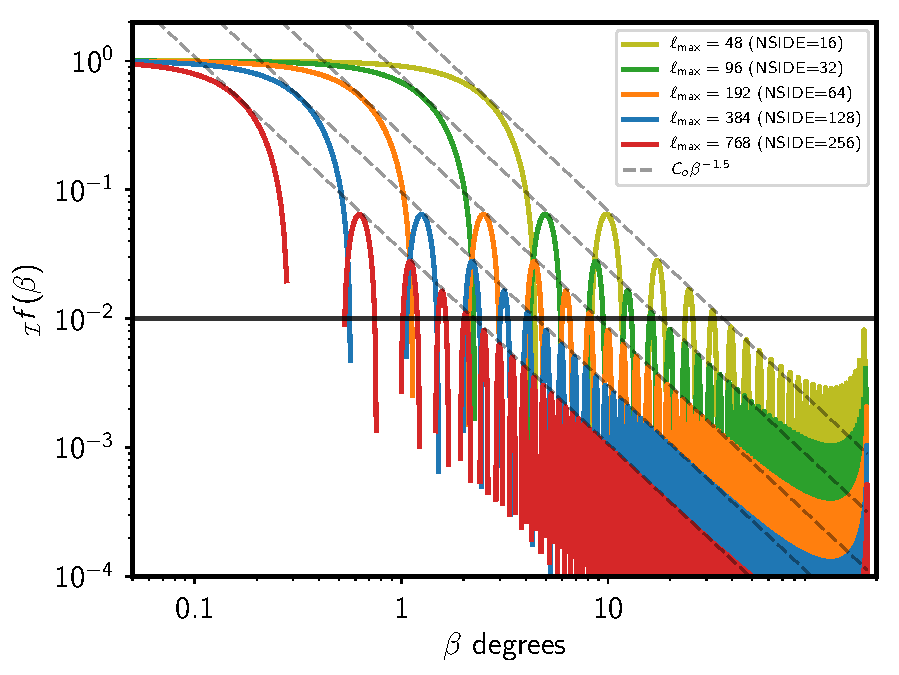
\includegraphics[width=0.48\columnwidth]{rad_ker_i_fn_of_ellmax.pdf}}
\subfigure{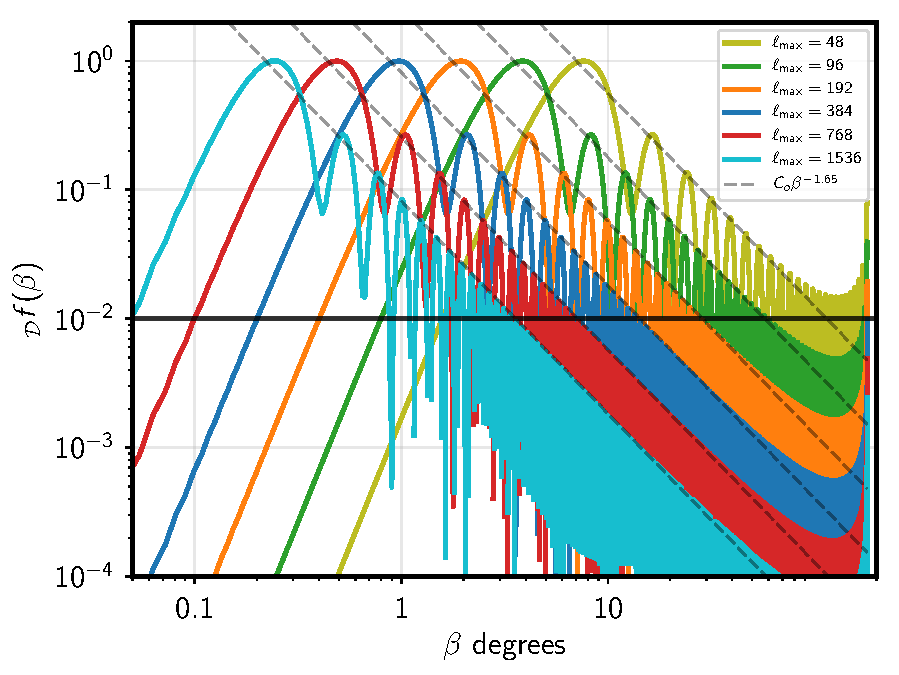
\includegraphics[width=0.48\columnwidth]{rad_ker_d_fn_of_ellmax.pdf}}
\caption{The top panel depicts the radial function  ${_{\mm}f}(\beta,\ell_{\rm min},\ell_{\rm max})$ while the bottom left and right panels show the radial functions ${}_{\mi}f(\beta,\ell_{\rm min},\ell_{\rm max}) ~\&~ {}_{\md}f(\beta,\ell_{\rm min},\ell_{\rm max})$ respectively, for fixed $\ell_{\rm min}=2$ and varying $\ell_{\rm max}$ as indicated by their legends. All the curves are normalized such that their maxima is set to unity. The horizontal solid black line marks the location where the amplitude of the respective kernels fall below 1\% of its maximum. The thin slanted dashed gray lines indicate a power law fit (by eye) to the envelope of the radial functions. The thick black short vertical dashed lines indicate the transition points as predicted by the empirically derived relation for the non-locality parameter $\beta_0=min(180,180 \frac{22}{\ell_{\rm max}})$.}
%While the envelopes for function ${_{\mm}f}(\beta)~\&~ {}_{\mi}f(\beta)$ are fit well by the power law $\propto \beta^{-1.5}$, the envelope for the function ${}_{\md}f(\beta)$ is seen to have a slightly steeper slope $\propto \beta^{-1.65}$.}
\label{fig:rad_ker_decay}
\end{figure}
%

${_{\mm}f}$ is the radial part of the kernel that translates the Stokes parameters $Q$ \& $U$ to scalars $E$ \& $B$ and vice versa and it has a vanishing contribution from the regions where ($\beta \rightarrow 0$) and from regions ($\beta \rightarrow \pi$) as seen in \fig{fig:beta_kernel}. This can be understood as arising from the fact that the coordinate dependence of the Stokes parameters cannot uniquely integrated out since the Euler angles $\alpha$ \& $\gamma$ are not uniquely defined at the locations $\beta=0,\pi$. This nature of ${_{\mm}f}$ is critical to ensure that the derived fields have the necessary spin properties.

\revisit{${_{\mi}f}$ is the radial part of the band limited delta function $\mi$ and expectedly has its maxima at $\beta=0$ and decays with increasing angular separation.  ${_{\md}f}$ has a vanishing value in the region where $\beta \rightarrow 0$ however it does not vanish at $\beta \rightarrow \pi$ as seen in \fig{fig:beta_kernel}. The main take away from these observations of the nature of the radial part of the kernel is that the real space operators which decompose the Stokes parameters into parts that correspond to E and B modes are necessarily non-local.}\\ \linebreak
\noindent \textit{The band limit dependence:} 
%It is clear from previous discussions that the scalar field $E$ \& $B$ constructed at a location depends on the Stokes field in the surrounding regions. 
We further quantify this non-locality by studying the radial extent of the kernels and its dependence on the maximum multipole accessible for analysis. To carry out this study we evaluate the radial functions for different values of $\ell_{\rm max}$, while keeping the lowest multipole fixed at $\ell_{\rm min}=2$. 

The resultant set of radial function are depicted in \fig{fig:rad_ker_decay}, where all the function have been normalized such that their global maxima is set to unity. The amplitude of these radial function scales up as $\propto \ell_{\rm max}^2$. Note that on increasing $\ell_{\rm max}$ the radial kernels shift left, attaining their global maxima at progressively small angular distances $\beta$.  At intermediate values of $\beta$, the envelope of the radial functions is fit well by a power law $ \propto \beta^{-n}$ as seen in \fig{fig:rad_ker_decay}.
In fact these finding are neatly summarized in the observation that the radial functions computed by evaluating the multipole sums to different maximum multipoles are self similar and follow this interesting telescoping and scaling property, $${}_rf(\beta,2,\ell_{\rm max}) \approx \Big[\frac{\ell_{\rm max}}{\ell'_{\rm max}}\Big]^2{}_rf(\beta'=\frac{\ell'_{\rm max}}{\ell_{\rm max}} \beta ,2,\ell'_{\rm max}) \,,$$ where ${}_rf$ denotes all the different radial functions. 
%We can understand the shifting left of the radial kernels on increasing the maximum multipole using this property. Lets say the function ${}_rf(\beta, \ell'_{\rm max})$ transition to being monotonously below some fraction of the global maxima at an angular distance of $\beta_0$.  The function ${}_rf(\beta', \ell_{\rm max})$, given $\ell_{\rm max} > \ell'_{\rm max}$, reaches the same transition point $\beta'=\beta_0$ at a smaller value of $\beta$ owing to the fact that $\ell_{\rm max}/\ell'_{\rm max}$ is greater than unity. The amplitude scaling of the functions is irrelevant since the transition point is always described in terms of the fraction of the global maxima of the function.

It is useful to define a characteristic radius of the region from which the evaluated resultant fields get most of their contribution.  Our primary interest is in quantifying the non-locality of the scalar modes $E$ \& $B$, therefore we define the abscissa at which the function ${_{\mm}f}(\beta,\ell_{\rm min}=2,\ell_{\rm max})$ transits to being monotonously below 1\% of the maxima of the function as the non-locality parameter: $\beta_{o}$.
%For $\ell_{\rm max}=24$, the maximum multipole accessible on a Nside=8 Healpix map, the non-locality parameter $\beta_0=180^{\circ}$ as the radial function never falls monotonously below 1\% of its global maxima as seen in \fig{}. Using this fact and the self similar property of the radial functions, we define the following empirical relation: $\beta_o= {\rm min}(180,180 \frac{24}{\ell_{\rm max}})$, as a means of estimating the non-locality parameter given the maximum multipole $\ell_{\rm max}$ accessible for analysis.
The simple empirical derived relation: $\beta_o= {\rm min}(180,180 \frac{22}{\ell_{\rm max}})$ provides a reasonable estimate of this transition point for  ${}_{\mm}f$. This empirical function also provides a reasonable estimate for the transition point for the function ${}_{\md}f$ particularly for high $\ell_{\rm max}$ and it systematically over-predicts the transition point for the function ${}_{\mi}f$ as seen in \fig{fig:rad_ker_decay}.
%--------------------------------------------------------
%--------------------------------------------------------
\section{Generalized polarization operators and recovering standard power spectra}\label{sec:generalized_operators}  
With our better understanding of the radial part of the kernel for CMB polarization, we can write down generalized $E/B$-like fields that depend on a different radial function, even one that we specify to have compact support.
The spin symmetry constrains the the azimuthal part of the real space kernels to be of the form $\sim e^{\pm i2 \alpha}$.  The radial parts of the stardard operators are determined by the sum over spherical harmonics and varies as a function of the band limit. It is here that we may potentially choose alternate forms for the radial functions to suit certain kind of analysis.

We can systematically generalize the real space operator by introducing the following harmonic space filter function:
%
\beq
\tilde{\mathcal{G}} = {\begin{bmatrix} g_{\ell}^E & 0  \\  0 & g_{\ell}^B \end{bmatrix}} \,,
\eeq
%
where the functions $g_{\ell}^E$ and $g_{\ell}^B$ represent the harmonic representation of the modified radial functions and can in the most general case be chosen to be different for $E$ and $B$ modes. To simplify discussions, we proceed by setting $g_{\ell}^E = g_{\ell}^B= g_{\ell}$. Given this harmonic function $g_{\ell}$, we can define the real space operator $\bar{O}'$ which translates Stokes $Q/U$ to $E/B$-like scalars (and the inverse operator $\bar{O}'^{-1}$) in the following manner,
% 
\begin{subequations} \label{eq:gen_qu2eb}
\beqry
{\bar O}' &=& {{}_0\mathcal{Y}} \, \tilde T^{-1} \tilde{\mathcal{G}} {{}_2\mathcal{Y}^{\dagger}} \, \bar T \,,\\
{\bar O}'^{-1}&=& \bar{T}^{-1} {{}_2\mathcal{Y}}\, \tilde{\mathcal{G}}^{-1} \tilde T {{}_0\mathcal{Y}^{\dagger}}.
\eeqry
\end{subequations}
%
The primed notation distinguishes these generalized operators from the default operators defined in \sec{sec:qu2eb} and \sec{sec:eb2qu}. We require both the forward and inverse operators to be well defined.   This constrains the choice of $\tilde{\mathcal{G}}$ to have a valid  inverse and is important to recover the standard CMB power spectra. The radial parts of this generalized operator and its inverse are given by the following expressions,
%
\begin{subequations}\label{eq:generalized_radial_kernel}
\beqry 
G_{QU \rightarrow EB}(\beta) &=& G(\beta) = \sum _{\ell=2} ^{\ell_{\rm max}} g_{\ell}\frac{2 \ell+1}{4 \pi} \sqrt{\frac{(\ell-2)!}{(\ell + 2)!}} P_{\ell}^2(\cos{\beta}) \, \label{eq:mod_rad_forward} \,, \\
G_{EB \rightarrow QU}(\beta) &=& G^{-1}(\beta) = \sum _{\ell=2} ^{\ell_{\rm max}} g_{\ell}^{-1}\frac{2 \ell+1}{4 \pi} \sqrt{\frac{(\ell-2)!}{(\ell + 2)!}} P_{\ell}^2(\cos{\beta}) \,. \label{eq:mod_rad_inverse}
\eeqry
\end{subequations}
%
The default radial function is just a special case resulting from the choice $\tilde{\mathcal{G}}=\mathbb{1}$ ($g_{\ell}=1$), in which case $\tilde{\mathcal{G}}^{-1}=\tilde{\mathcal{G}}$ and therefore $G^{-1}(\beta) = G(\beta)={{}_{\mm}f}$.

While defining these generalized operators, it is more natural to choose the real space function $G(\beta)$ rather than the harmonic space $g_l$, bearing in mind the constraint that $G(\beta=0)=G(\beta=\pi)=0$. Employing the orthogonality property of associated Legendre polynomials it can be shown that the harmonic function $g_{\ell}$ is given by the expression,
%
\beq
g_{\ell} = 2 \pi \sqrt{\frac{(\ell-2)!}{(\ell+2)!}} \int _{0}^{\pi} G(\beta) P_{\ell}^{2}(\cos{\beta}) d\cos{\beta} \,. \label{eq:gb2bl}
\eeq
%


An arbirtrary $G(\beta)$ for which $g_{\ell} \neq 1$ can be equivalently thought in terms of the standard $E/B$ fields being convolved with some effective circularly symmetric beam whose radial profile is given by the expression,
%
\beq
b(\beta) = \sum_{\ell=0}^{\ell_{\rm max}} \frac{2 \ell+1}{4 \pi} g_{\ell} P_{\ell}^{0} (\cos{\beta})\,,
\eeq
%
where $g_{\ell}$ is the same harmonic function as that appearing in \eq{eq:generalized_radial_kernel}.
In contrast to the radial function $G(\beta)$ an instrumental beam function appropriately normalized has the property $b(\beta) \rightarrow 1$ as $\beta \rightarrow 0$. Though the real space functions $G(\beta)$ (operating on Stokes parameters) and $b(\beta)$ (operating on scalar $E/B$) are different, in harmonic space they play identical roles.
%
\begin{figure}[!t] 
\centering
\subfigure[\label{fig:gl_gbeta}]{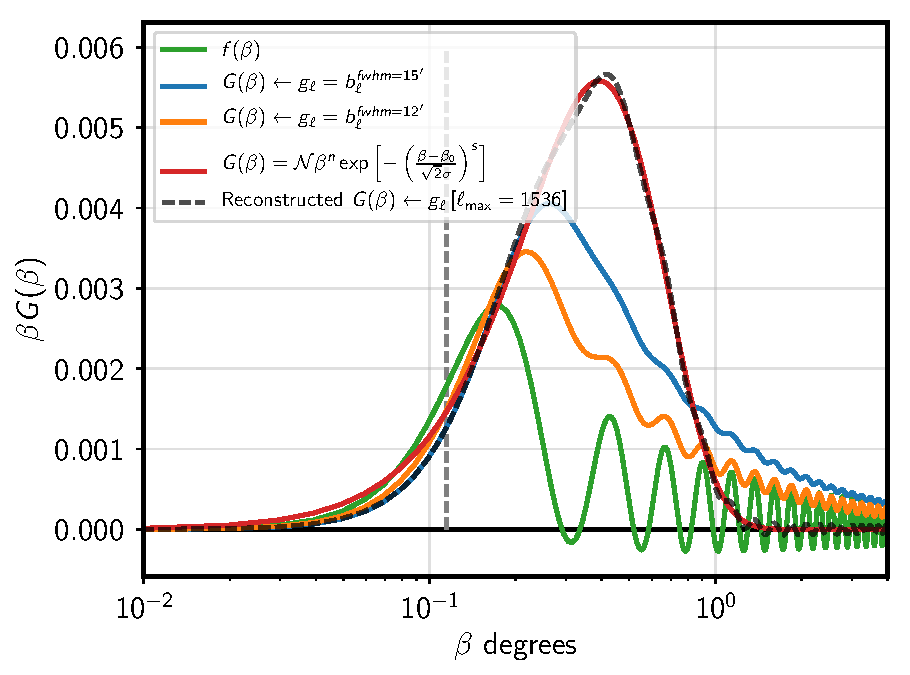
\includegraphics[width=0.48\columnwidth]{Gbeta_for_different_gl_lmax1536.pdf}}
\subfigure[\label{fig:glbl}]{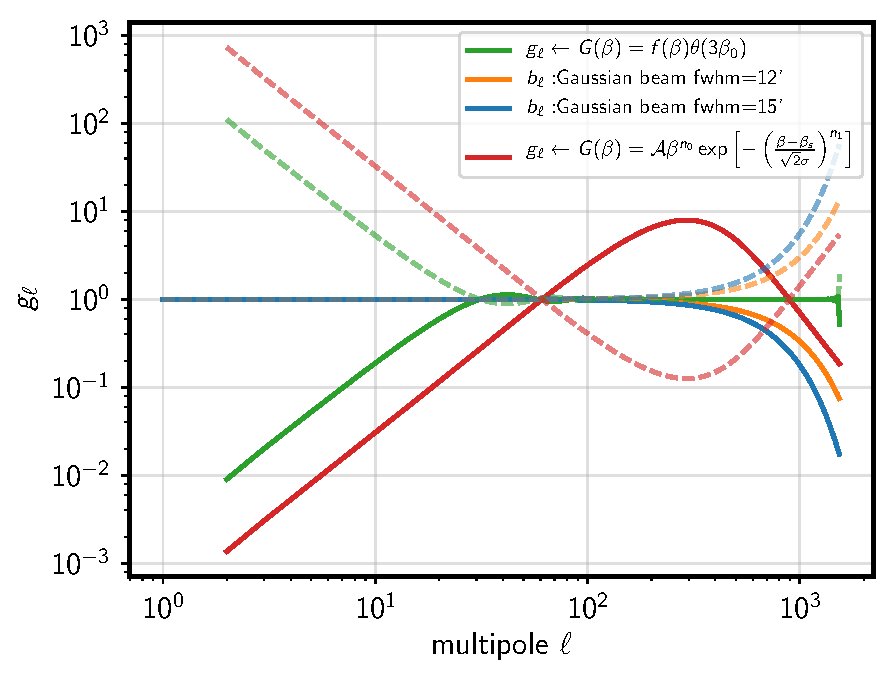
\includegraphics[width=0.48\columnwidth]{gl_for_different_gbeta_lmax1536.pdf}}
\subfigure[\label{fig:gl_bbeta}]{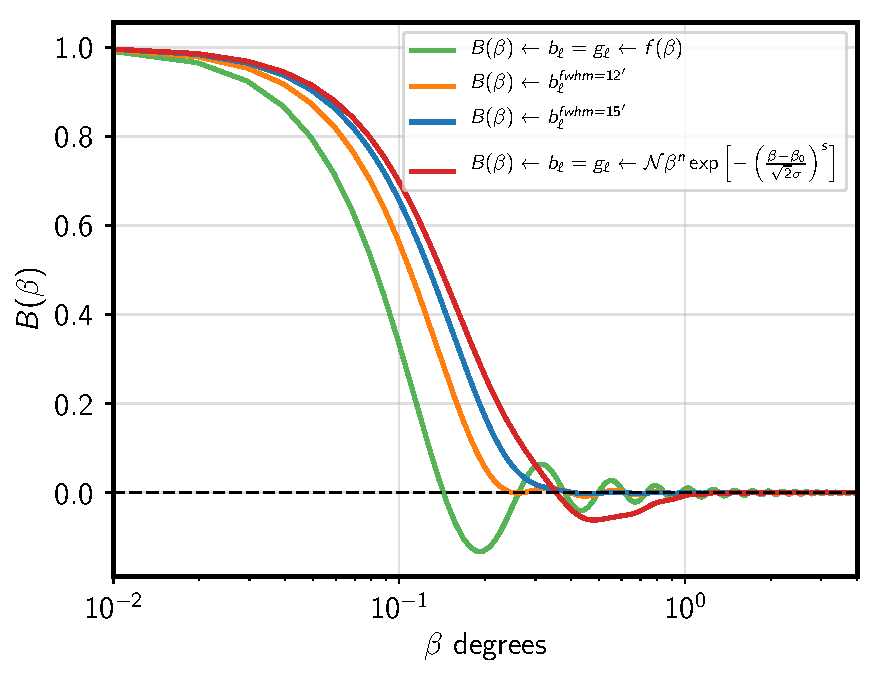
\includegraphics[width=0.48\columnwidth]{Bbeta_for_gl_lmax1536.pdf}}
\caption{\textit{Top left:} The green line depicts the default radial kernel $f(\beta)$ defined in \eq{eq:qu2eb_gen_kernel}, multiplied by an apodized step function $\theta(3 \beta_0)$. The blue and orange lines depict the modified radial function resulting the beam harmonics $b_{\ell}$ corresponding to Gaussian beams with fwhm=15 \& 12 arc-minutes respectively. The red curve depicts an example modified radial function: $G(\beta)=\mathcal{A} \beta^{n_o} \exp{\left[ -\left( \frac{\beta-\beta_s}{\sqrt{2} \sigma} \right)^{n_1} \right]}$ with parameters set to the following values $[n_0=1;\, \beta_s=0 ;\, \sigma = 0.004 ;\, n_1=1.5]$. The black dashed curve depicts the band limited reconstruction of the modified radial function. \textit{Top right:} This figure depicts the normalized beam function $b(\beta)$ evaluated from interpreting the respective harmonic functions as those corresponding to an effective instrument beam.  \textit{Bottom:} This figure depicts the harmonic representation of the respective radial functions as indicated by the legend. The dashed curves of the corresponding color depict the inverse of the harmonic functions.}
\label{fig:example_gbeta}
\end{figure}
%

% Therefore it is possible to interpret the beam harmonic coefficients as those representing some modified radial kernel.
In \fig{fig:example_gbeta}, we examine in more detail the relationship between the modified radial kernels and these beam harmonic coefficients.  
 \fig{fig:gl_gbeta} depicts the radial profile of the  effective beams corresponding to different radial kernels: the standard kernel with a radial cutoff, kernels corresponding to Gaussian smoothings of the $E/B$ fields, an radial function without oscillations and an exponential cutoff.  Note that the smoothing tend to increase the non-locality, indicated by the shifting right of the maxima of the respective kernels, as one may have expected.  The exponential cutoff (red curve) by construction has a very small non-locality (parameterized by $\beta_0$).

\fig{fig:glbl} depicts the harmonic description $g_{\ell}$ for these respective radial kernels and beams.
Finally, the beam that the modified radial kernels appies to the $E/B$ fields we show in \fig{fig:gl_bbeta}.  Note that the beam function corresponding to the default radial kernel ($g_{\ell}=1$) is merely a band limited representation of a delta-function beam.
%In \sec{sec:local_conv_eb} we constructed localized convolution kernels by multiplying $R(\beta)$ with an apodized version of the step function $\theta_{\rm apo}(r_{\rm cutoff})$. The oscillation seen in the spectra in \fig{fig:eb-spectra_rad_cutoff} can be explained to be due to this effective beam characterized by $g_{\ell}^2$ operating on the power spectra. The effective beam can be evaluated by computing the multipole function $g_{\ell}$ as follows,
%%
%\beq
%g_{\ell} = 2 \pi \sqrt{\frac{(\ell-2)!}{(\ell+2)!}} \int _{0}^{r_{\rm cutoff}} R(\beta) \theta_{\rm apo}(r_{\rm cutoff})  P_{\ell}^{2}(\cos{\beta}) d\cos{\beta} \,, \label{eq:gb2bl} \,,
%\eeq
%%
%where the upper limit of the integration is set to $r_{\rm cutoff}$ since the function $\theta_{\rm apo}(r_{\rm cutoff})$ vanishes for $\beta>r_{\rm cutoff}$. The function $b^2_{\ell}-1$ matches the oscillation seen in \fig{fig:eb-spectra_rad_cutoff} as  seen in \fig{fig:match_cl_oscillations} where the two results have been over plotted.
%%
%\begin{figure}[!t] 
%\centering
%\subfigure[]{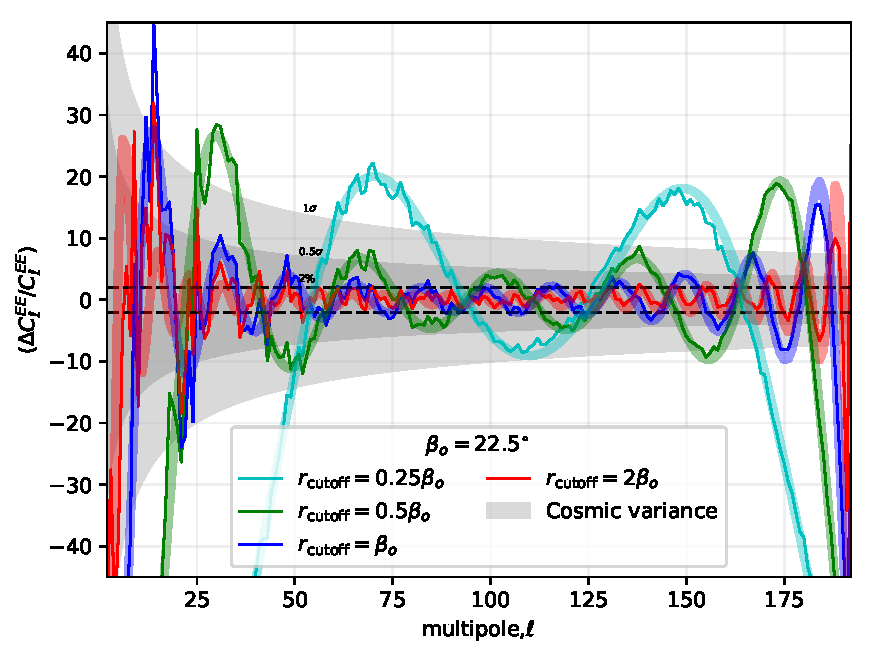
\includegraphics[width=0.98\columnwidth]{analytical_cl_oscillations_vs_data.pdf}}
%\caption{The thin lines depicts the same spectral differences as those seen in \fig{fig:eb-spectra_rad_cutoff}, while the thick lines of the corresponding color depict the function $g_{\ell}^2 -1$ as derived from evaluating \eq{eq:gb2bl} for different $r_{\rm cutoff}$}.
%\label{fig:match_cl_oscillations}
%\end{figure}
%%
%The apodized step function in this case transition from 1 at $\beta < r_{\rm cutoff} -w$ to 0 at $r_{\rm cutoff}$ over a width $w= 3^{\circ}$ with a cosine squared profile .

%--------------------------------------------------------
%\subsubsection{Recovering the standard $E$ and $B$ mode spectra}

The generalized convolution kernels defined in the previous section, when operated on the Stokes vector returns some scalar $E'$ and $B'$ mode maps,
%
\beq
\bar{S}' = \bar{O}' \bar{P}
\eeq
%
which are merely filtered versions of the standard $E/B$ modes maps. Since the filter function is simply $g_{\ell}$, easily obtained from the modified radial function $G(\beta)$, and it can be simply interpreted as the harmonic coefficients of some azimuthally symmetric beam, the power spectra of the modified scalar fields $E'$ and $B'$ are related to the spectra of the standard $E$ and $B$ fields via the following relation, 
 %
 \begin{subequations}
 \beqry
C_{\ell}^{EE,BB,EB} &= &C_{\ell}^{E'E',B'B',E'B'} /   g_{\ell}^2\,,\\
C_{\ell}^{TE,TB}  &=&  C_{\ell}^{TE',TB'} / g_{\ell}\,,
 \eeqry
 \end{subequations}
 %
 where $C_{\ell}$ denotes the angular power spectra and $T$ refers to the temperature anisotropy map. Therefore the standard CMB spectra can always be recovered as long as the $1/g_{\ell}$ and $1/g_{\ell}^2$ are well behaved functions, which can be ensured by making a suitable choice for the modified radial function $G(\beta)$. %Some examples forms of $G(\beta)$, its harmonic representation $g_{\ell}$ (and its inverse $1/g_{\ell}$ ) and the corresponding beam $B(\beta)$ are depicted in \fig{fig:example_gbeta}.
%One direct application of this freedom in choosing the radial kernel is that one can mitigate the issue of leakage of power from $E$ to $B$.  By constructing a radial function which tapers to zero at sufficiently small radii one can clearly discard pixels which are affected by masking. 
%--------------------------------------------------------

%--------------------------------------------------------
\paragraph{Relation to the spin raising $\eth^2$ and lowering $\bar{\eth}^2$ operators.}
Recall that on operating twice with the spin lowering operator on the Stokes charge ${}_{+2}X$ results in filtered version of $E/B$ maps as in \eq{eq:ebdef}. Now note that it is possible to construct a modified real space operator by choosing the harmonic space function to be $g_{\ell} = ({(\ell+2)!/(\ell-2)!})^{1/2}$, resulting in similarly filtered $E/B$ maps as follows:
%
\beq 
[\mathcal{E} + i \mathcal{B}](\hat{n}_e)=- \Delta \Omega\sum_{q=1}^{N_{\rm pix}} \Bigg\lbrace  \left[  \sum_{\ell=\ell_{\rm min}}^{\ell_{\rm max}} \frac{2 \ell+1}{4 \pi} P_{\ell}^2(\beta_{qe}) \right] e^{-i2\alpha_{eq}} {}_{+2}X(\hat{n}_{q}) \Bigg\rbrace \,.\label{eq:bl_ebdef_lower} 
\eeq
%
Comparing \eq{eq:ebdef_lower} to \eq{eq:bl_ebdef_lower} makes apparent the following mapping:
%
\beq
\bar{\eth}^2 \equiv \Delta \Omega \sum_{q=1}^{N_{\rm pix}} \left[ \sum_{\ell=\ell_{\rm min}}^{\ell_{\rm max}} \frac{2 \ell+1}{4 \pi} P_{\ell}^2(\beta_{qe}) \right] e^{-i2\alpha_{eq}}\,.
\eeq
%
The operator $\bar{\eth}^2$ is composed of derivative operations and hence has an implicit positional dependence for all numerical purposes which is made explicit in the band limited version of the operator.  The band limited version of the spin raising operator $\eth^2$ is derived by simply taking the conjugate of the above equation.
%--------------------------------------------------------

\section{Discussion}\label{sec:discussion}
In this work, we presented a first derivation of the real space operators on the sphere that transform the Stokes polarization vector to into a vector of scalars and vice versa.  We also presented real space operators that directly decompose the full Stokes vector \vp{} into vectors \vp{E} and \vp{B} that correspond to the respective scalar modes.  To facilitate these derivations we introduced a vector-matrix notation which allows for concise book keeping of all the standard operations involved in the analysis of  polarization maps (or any spin-2 fields) on the sphere. This real-space analysis method trivially generalizes to maps of arbitrary spin.

These real space operators offer a spatially intuitive way of understanding the different decompositions of the Stokes vector on the sphere. We explicitly  demonstrated that all the real space operators are separable into azimuthal and radial parts. While the azimuthal part of the operators is primarily responsible for handling the spin decomposition, the radial weights determine the non-local dependence of the resulting fields on the original fields.  Only the radial part of the kernel depends on the band limit. 
The radial parts of the operator kernels are roughly self-similar in the sense that the radial kernels evaluated with some band limit are related to other radial kernels (evaluated with a different band limit) by an approximate rescaling of the function. We use this property to define a non-locality parameter $\beta_0$ as the angular distance at which the amplitude of the radial kernel falls below one percent of its maxima and it  is a function of the maximum multipole $\ell_{\rm max}$ available for the analysis. We empirically show that the non-locality parameter is approximately given by: $\beta_0 = \mathrm{min}(180^{\circ}, 180^{\circ} \frac{\ell_{0}}{\ell_{\rm max}})$ with $\ell_{0}=22$ for the operator that converts Stokes Q/U to scalars E/B and vice versa (see \fig{fig:rad_ker_decay}). An analysis in  \cite{Zaldarriaga2001a} treated real space $E/B$ operators in the flat sky.  It did not explicitly derive the radial part of the kernel, but argued on geometric grounds that it should fall with angular separation as $\beta^{-2}$.  We find that this agrees with the average behavior of radial functions after averaging oscillations and note that some such averaging always takes place in practice due to pixelization of the signal.  However, for precision reconstruction of $E/B$ on the sphere, the oscillations must be taken into account.

Our careful study of the real space operators show that they can be expressed either as Green's functions or as convolving beam functions.  The convolution interpretation is not a totally new concept.  It guides the discussion in \cite{Zaldarriaga2001a} and closely relates to the popular spokes and pinwheel descriptions of the $E/B$ modes.  However, the radiation/Green's function interpretation of the operators is a new one and is discussed here for the first time in detail on the sphere. These two different interpretations of the operators emerge from the expression of the kernels in terms of the forward or inverse rotation Euler angles.  The mathematical forms of the Green's function and convolution kernels swap roles (and are conjugated) when transforming back to $Q/U$ from $E/B$.

The Green's function interpretation provides some useful insights into these operations. In particular it allows us to think of ${}_{+2}X=Q+iU$ as some spin-2 charge which radiates out a complex spin-0 scalar field $E+iB$. The resulting complex scalar maps can be then understood as arising from superposition of the radiated spin-0 scalar fields emanating from all the spin charges on the sphere.  The $E/B$ mode maps are merely the real and imaginary parts of this field. Results that demonstrate the equivalence of these real space methods to the conventional harmonic space methods will be presented in the next paper in this series.

Deeper understanding of the non-locality of the real space operators has allowed us to generalize the real space operators that transform between the spin-2 and spin-0 representations of the CMB polarization. We presented a systematic procedure to modify and generalize the construction of the scalar polarization fields and to control the radial kernels, specifying them with few restrictions.  We argue that these modifications to the radial kernel have the same effect as a smoothing operation on the $E/B$ fields by a circularly symmetric beam.  Therefore it is trivial to recover the standard CMB angular power spectra from the modified scalar polarization maps resulting from the modified kernels.  We noted that the standard spin-raising ($\eth^2$) and spin-lowering ($\bar{\eth}^2$) operators are special cases of these generalized operators which allowed us to present a band limited representation of these operators. 

Modified real-space operators with compact kernels could open several alternative analysis routes in the future.  No spin-harmonic transforms are necessary as the real space operators only rely on computing the Euler angles which can be done on the fly.  The radial functions (depending on $P_{\ell}^{2}$) need be tabulated only once at some determined resolution.  Especially given the Green's function interpretation of these operators, their implementation is trivially parallelizable over a compact domain, since the $E/B$ contribution from the Stokes charges in each pixel can be evaluated independently.  Alternatively, the spatially-varying convolution kernel could be applied a polarized effective beam, as implemented in \cite{2011ApJS..193....5M} in a parallel scheme.

The real space kernels could in principle be incorporated into the pointing matrices for map making, allowing maps of $E/B$ to be made directly from instrument data, without the need for Stokes parameter maps as intermediate products.
  The pointing matrix---projecting the maps into the time-ordered data at a point---requires the convolution version of the kernel, while the transpose pointing matrix---projecting the time-ordered data to the map---requires the Green's function kernel.
  The method would be similar to pixel-based strategies to deconvolve an instrument beam during map making \citep[e.g.][]{2010ApJS..187..212C}. Such a strategy for map making would result in the pointing matrix in being much less sparse, hence making a practical implementation significantly challenging. Using the compact radial kernels might help with restoring some of the sparseness of the pointing matrix, however a real world implementation of this method requires a more careful feasibility study.
  %However, such a strategy for map making would force the pointing matrix to be much less sparse and it may not be practical.
 
Since the real space operators let us tune the locality of $E/B$ maps, this can be potentially exploited to eliminate foreground contamination from distant parts of the sky. Such applications can be difficult to implement using conventional harmonic space methods.  For instance, the real space operators can be defined such that the locality of their radial kernels is varied on different portions of the sky, dictated by say the foreground morphology, resulting in some modified scalar $E'/B'$ maps.  While this idea seems interesting, the usefulness of this implementation will depend on whether the standard $E/B$ mode spectra are easily recoverable in this fashion.  We will explore some of these possible analysis directions in the future papers of this series.

Finally, the toolbox of real-space operators gives us more intuition about the $E$- and $B$-mode structure of polarized gas and dust filaments in the Milky Way, an important foreground for inflationary science. We demonstrate that filaments with finite length or changing radius of curvature result in $B$-mode patterns in addition to the $E$-mode pattern already expected.  We therefore predict a characteristic $B$-mode pattern from filament sources that should be observable in future polarization measurements.

%\appendix
%\section{Appendix}
%%--------------------------------------------------------
%%--------------------------------------------------------
%\subsection{Product of spin spherical harmonics}\label{sec:ylm_prod}
%The spin spherical harmonics are related to the Wigner D functions via the following relations,
%%
%\beq
%D_{-s m}^{\ell}(\alpha,\beta,\gamma) = \sqrt{\frac{4 \pi}{2 \ell+1}} {}_{s}Y_{\ell m }(\beta,\alpha)e^{-is\gamma} \,,
%\eeq
%%
%where $\alpha, \beta~\&~\gamma$ can be thought of as Euler angles for some rotation.
%
%The product of two different spherical harmonic functions can be expressed in terms of the Wigner D functions and simplified using their identities. In particular we are interested in products of spherical harmonic function of the following kind,
%%
%\begin{subequations}
%\beqry
%\sum_{m} {}_{s_1}Y_{\ell m }(\theta_e,\phi_e) {}_{s_2}Y^*_{\ell m }(\theta_q,\phi_q) &=& \frac{2\ell+1}{4 \pi}  \sum_{m}D^{\ell}_{-s_1 m }(\phi_e,\theta_e,0) D^{*\ell}_{-s_2 m }(\phi_q,\theta_q,0) \,,\\
%&=& \frac{2\ell+1}{4 \pi}  \sum_{m}D^{\ell}_{-s_1 m }(\phi_e,\theta_e,0) D^{\ell}_{m -s_2 }(0,-\theta_q,-\phi_q) \,, \\
%&=& \frac{2\ell+1}{4 \pi} D^{\ell}_{-s_1 -s_2 }(\alpha_{qe},\beta_{qe},\gamma_{qe}) \,, \\
%&=& \sqrt{\frac{2\ell+1}{4 \pi}} {}_{s_1}Y_{\ell -s_2}(\beta_{qe},\alpha_{qe}) e^{- i s_1 \gamma_{qe}}
%\eeqry
%\end{subequations}
%%
%where we have used some standard identities of the Wigner D functions to transition between then  equations \cite{varshalovich}. Note that the Euler angles $(\alpha,\beta,\gamma) = (0,-\theta_q,-\phi_q)$ correspond to a rotation that aligns the local cartesian coordinate at $\hat{n}_q$ with that at the pole and the Euler angles $(\alpha,\beta,\gamma) = (\phi_e,\theta_e,0)$ correspond to rotations that align the local cartesian coordinates at the pole with those at the location $\hat{n}_e$. Hence the net rotation operation is that of aligning the local cartesian coordinates at location $\hat{n}_q$ with those at location $\hat{n}_e$ and therefore the final results are expressed in terms of Euler angles: $(\alpha_{qe},\beta_{qe},\gamma_{qe})$.
%
%Since the following equation holds true,
%\beq
%\sum_{m} {}_{s_1}Y_{\ell m }(\theta_e,\phi_e) {}_{s_2}Y^*_{\ell m }(\theta_q,\phi_q) = \sum_{m} {}_{-s_1}Y^*_{\ell m }(\theta_e,\phi_e) {}_{-s_2}Y_{\ell m }(\theta_q,\phi_q) \,,
%\eeq
%this sum over product of spin spherical harmonic functions can be equally expressed in terms of the Euler angles corresponding to the inverse rotations. Using the same algebra as given above, \revisit{it is possible to show that }


%%--------------------------------------------------------
%%--------------------------------------------------------
%\subsection{Relation between the real space operators and the spin raising/lowering operators}\label{sec:operator_connection}
%%--------------------------------------------------------
%%--------------------------------------------------------
%\subsection{ Mathematical properties of spin spherical harmonics}\label{sec:ylm_mathprop}
%The sum over $m$ index of product of two spherical harmonic functions of spin $s_1$ and $s_2$ respectively, is given by the following expression \cite{varshalovich},
%\beq \label{eq:sum_spin_shf}
% \sum_{m}{_{s_1}Y^*_{\ell m}}(\hat{n}_i){_{s_2}Y_{\ell m}}(\hat{n}_j) = \sqrt{\frac{2\ell+1}{4 \pi}} _{s_2}Y^{-s_1}_{\ell}(\beta,\alpha) e^{- i s_2 \gamma} \,,
%\eeq
%where $\alpha, ~\beta ~\&~ \gamma$ correspond to the Euler angles that specify the rotation matrix which transforms the local cartesian coordinates defined at $\hat{n}_i$ such that it aligns with the local cartesian coordinate system at $\hat{n}_j$.
%
%The spin spherical harmonics satisfy the following orthogonality relations,
%%
%\beq
%\int  {_sY_{\ell m}}(\hat{n}){_sY^*_{\ell' m'}}(\hat{n}) d\Omega = \delta_{\ell \ell'} \delta_{\rm m m'} \,, \label{eq:ylmortho1}
%\eeq
%%
%where $s$ denotes the spin of the spherical harmonic coefficients. The numerical validity of \eq{eq:ylmortho1} is only limited by the rate at which these functions are sampled on the sphere and hence this identity can be made arbitrarily accurate by choosing a sufficiently high sampling rate.
%%While working with CMB polarization one is often dealing with spin-2 spherical harmonics. Here we derive some relation which we use while evaluating the real space projection operators,
%%\beq
%%\sum_{\ell m} {_2Y}_{\ell m}(\hat n_i) {_2Y}^*_{\ell m}(\hat n_j) = 
%%\eeq
%
%The spin spherical harmonic functions satisfy the following completeness relation,
%%
%\beq
%\sum_{\ell m}{_sY_{\ell m}}(\hat{n}_i){_sY^*_{\ell m}}(\hat{n}_j) = \delta(\hat{n}_i - \hat{n}_j) \label{eq:ylm_prop1} \,,
%\eeq
%%
%Note that the numerical validity of \eq{eq:ylmortho2} is strictly true only when the sums over the indices $(\ell, m)$ run to infinity. This is never true in practice, since the measured data invariable are band limited owing to the finite resolution of the experiments. Hence this relation is only approximately true and in more realistic scenario takes up the following function form,
%%
%\beqry
%\sum_{\ell=\ell_{\rm min}, m}^{\ell_{\rm max}}{_{s_1}Y^*_{\ell m}}(\hat{n}_i){_{s_2}Y_{\ell m}}(\hat{n}_j) &\approx& \delta(\hat{n}_i - \hat{n}_j) \label{eq:ylmortho2} \,, \\
%\sum_{\ell=\ell_{\rm min}, m}^{\ell_{\rm max}}{_{s_1}Y^*_{\ell m}}(\hat{n}_i){_{s_2}Y_{\ell m}}(\hat{n}_j) &=& \sum_{\ell=\ell_{\rm min}}^{\ell_{\rm max}} \sqrt{\frac{2 \ell+1}{4 \pi}} {}_{s_2}Y^{-s_1}_{\ell}(\beta,\alpha) e^{-i s_2 \gamma} \,, \nonumber
%\eeqry
%%
%where $\alpha, \beta ~\&~ \gamma$ are the Euler angles. A specific case of this function with $(s=2, \ell_{\rm min}=2, \ell_{\rm max}=96)$ is depicted in the last two columns of \fig{fig:vis_kernel}.
%%--------------------------------------------------------
%%--------------------------------------------------------
%
%%--------------------------------------------------------
%%--------------------------------------------------------
%\subsection{The flat sky limit}\label{sec:flat_sky}
%%--------------------------------------------------------
%%--------------------------------------------------------


\bibliographystyle{JHEP}
\bibliography{ref}

\end{document}